\documentclass[double,12pt]{beavtex}
\usepackage{graphicx}
\usepackage{rotating} %Package added to allow the rotation of figures and chart on a page, {sidewaysfigure} command
\usepackage{tablefootnote} %Packaged added to allow footnotes in the tabular environment, use \tablefootnote command
\title{Freezing of a Weeks-Chandler-Anderson Fluid using classical Density Functional Theory}
\author{Kirstie L. Finster}
\degree{Master of Science}
\doctype{Thesis}
\department{Physics}
\depttype{Department}
\depthead{Head}
\major{Physics}
\advisor{David Roundy}
\submitdate{October ??, 2020}
\commencementyear{2021}

\newcommand\davidsays[1]{\textcolor{red}{[\it D: #1]}}

\usepackage{color}
\usepackage{amsmath}
\usepackage{subcaption}

\date{October 2020}

\abstract{
  We use Classical Density Functional Theory (cDFT) to predict the 
  freezing of a Weeks-Chandler-Anderson (WCA) fluid. A WCA fluid 
  consists of soft spheres that exhibit the repulsive portion of the 
  Leonard-Jones potential widely used to model the interaction of two 
  neutral atoms. Our cDFT functional is constructed using Soft Fundamental 
  Theory (SFMT) with Tarazona's tensor expression for $\Phi_3$, and Schmidt's
  erf model in which we have incorporated temperature dependent
  parameters to
  \davidsays{fit the results to those predicted by Monte-Carlo simulations}.
  Our functional was successful in predicting the freezing of the WCA fluid 
  with a fairly good match to Monte-Carlo simulations. This result suggests 
  that SFMT may provide a solid foundation for future density functionals 
  that will model real fluids.
}

\begin{document}
   \maketitle
   \mainmatter

\chapter{Introduction}

The goal of this project is to generate temperature-density 
and pressure-temperature phase diagrams for a Weeks-Chandler-Anderson (WCA) 
model fluid using classical Density Functional Theory (cDFT). 
To do this, the Helmholtz free energies of the fluid
in a liquid state and in a crystalline solid state must be found.
In general, the Helmholtz free energy, which consists of an ideal part 
and an excess part, can be written as a functional of the number density 
profile $n(\vec{r})$ which describes the way the average number 
density varies spatially. 
\begin{equation}{F[n(\vec{r})]=F_{ideal}[n(\vec{r})] + F_{excess}[n(\vec{r})]}\end{equation} 

Soft Fundamental Measure Theory (SFMT) will be used to form the 
functional for the excess Helmholtz free energy. 
SFMT is a method that makes the task of 
forming an expression for the excess Helmholtz free energy of a particular 
model fluid much easier since the interaction that each sphere, or atom, 
has with every other sphere does not have to be taken explicitly into account.
Once the functional for the Helmholtz free energy is formed, classical 
Density Functional Theory is used to find the equilibrium 
Helmholtz free energy at a particular temperature and density. 
According to cDFT the equilbrium 
Helmholtz free energy of the system can be found by varying the number 
density profile $n(\vec{r})$ until the free energy is minimized. 
Results will be compared to those from Monte-Carlo simulations.

\chapter{Theory}

\section{Model Fluids and the Weeks-Chandler-Anderson Fluid (WCA)}

Real fluids and their behavior are very complex from a physicist's point 
of view. Although a water molecule, for example, is composed of only three
atoms, the ever-changing redistribution of charges within the molecules, 
and their interaction with charges from other molecules make it difficult 
to study a fluid composed of water molecules directly. The task becomes 
even more daunting considering the complicated molecular motion of each 
water molecule, and the sheer number of molecules that must be taken 
into account. 
The problem of understanding the behavoir of real liquids is better addressed 
by using models which reduce a complex picture to a simple one. Modifications, 
or perturbations, can then be incorporated into the model making it 
progressively more complex until it mimics the behavior of a real 
liquid as closely as possible.

In developing a model for a fluid, simplifications can be made regarding 
the composition, type, shape, and interatomic interaction of the molecules. 
Rather than dealing with any particular molecule or atom, the model only 
deals with generic ``particles", which may also be referred to as ``atoms''. 
The shape of the particles, or atoms will be the simplest shape possible - 
a sphere. The spheres in the simplest models do not exhibit quantum 
interference effects as the mass of the spheres, and the temperature 
are taken to be large enough that the de Broglie wavelength is smaller 
than the mean distance between the spheres. The fluid can then be treated 
as a classical fluid where the spheres interact with each other according 
to their electrostatic interatomic potential. 

There are many interatomic potentials which can be used to model a fluid 
each of which describes the interaction between two real atoms to some 
degree of accuracy. The simplest, and oldest, model used to describe a 
fluid is the hard-sphere model. The hard-sphere model envisions a fluid 
to be composed of hard spheres like, for example, a collection of marbles. 
This model came about by considering the near incompressibilty of liquids 
indicating that the particles making up the liquid strongly resist being 
pushed closer together. This behavior can be described by an interatomic 
potential energy that is zero when two spheres are not in contact, but 
goes instantly to infinity when contact is made. The inablilty to push 
real atoms closer together is due to the repulsion of the electrons in 
each atom, and is the dominating interparticle electrostatic interaction. 
Thus, the hard-sphere model - which is the simplest, but still effective 
representation of this replusive behavior that dominates the interaction 
between real atoms, is currently the most widely used model for fluids.

\begin{figure}[h!]
    \centering
    \includegraphics[height=7cm]{plot_HardSphere_Potential.pdf}
    \caption{A Hard Sphere Potential is zero for $r>2R$, and infinity 
    for $r\leq{2R}$ where R is the radius of a hard sphere (which is 
    approximately 1.225/2 in this example).}
    \label{fig:HardSphere_potential}
  \end{figure}

Another fairly simple, but relatively accurate interatomic potential widely 
used to represent generic, neutral atoms is the Leonard-Jones potential. 
The Leonard-Jones potential describes both the long-range attraction, 
and the short-range replusion that occurs between two nuetral atoms. 
The attraction between two nuetral atoms is due to fleeting dipoles that 
form spontaneously when electrons are redistributed as atoms come into 
close proximty. These are often characterized as Van der Walls, or London 
dispersion forces. The attraction grows stronger as two atoms move closer 
together until their atomic orbitals begin to overlap. 
At this point the electrons in each atom begin to oppose the overlap of 
the two atoms through their replusion. The repulsion increases rapidly and 
approaches infinity as the distance between the atoms conintues to decrease.  
 
\begin{figure}[h!]
    \centering
    \includegraphics[height=7cm]{LJ_Potential.pdf}
    \caption{Leonard-Jones Potential for $\sigma=1$, $\epsilon=1$}
    \label{fig:LJ_potential}
  \end{figure}

The combined attractive and repulsive effects produce the overall shape of 
the Leonard-Jones interatomic potential shown in Figure \ref{fig:LJ_potential}. 
The potential is zero when the distance r between the centers of two atoms 
is equal to $\sigma$ (shown in the figure at r/$\sigma$=1). At this point 
the attraction bewteen the atoms just cancels their repulsion. As the distance 
between the centers of the two atoms decreases below $\sigma$, the potential 
rapidly approaches positive infinity corresponding to infinite repulsion. 
Above $\sigma$ the potential becomes negative indicating a net attraction 
between the atoms. The net attraction is maximized at a distance of 
r=$2^\frac{1}{6}\sigma=2R\approx{1.122}\sigma$ where R is the radius of 
the sphere given by $R={2^{-\frac{5}{6}}}\sigma$. At this point the depth of
the potential well, given by epsilon $\epsilon$, is a maximum. As r increases 
further, the net attraction decreases and the potential approaches zero
asymptotically. The attractive and repulsive effects can be separated into two
potentials, shown with different colors in Figure \ref{fig:LJ_potential_2parts}, 
which when added together regenerate the full Leonard-Jones potential. 

\begin{figure}[h!]
    \centering
    \includegraphics[height=7cm]{LJ_Potential_2part.pdf}
    \caption{Leanard-Jones Potential broken into two parts for $\sigma=1$, $\epsilon=1$}
    \label{fig:LJ_potential_2parts}
  \end{figure}

\begin{figure}[h!]
    \centering
    \includegraphics[height=7cm]{WCA_Potential.pdf}
    \caption{WCA Potential for $\sigma=1$, $\epsilon=1$}
    \label{fig:WCA_potential}
  \end{figure}

The repulsive portion of the Leonard-Jones potential forms the potential for a 
Weeks-Chandler-Anderson (WCA) model fluid~\cite{andersen1971relationship}, 
shown in Figure \ref{fig:WCA_potential}. 
The WCA potential is described by the equation: 
\begin{equation}{V_{WCA}=\left\{\begin{array}{rcl} {4\epsilon{\left[\left(\frac{\sigma}{r}\right)^{12} - \left(\frac{\sigma}{r}\right)^6 \right]}+\epsilon} & \mbox{for} & 0<r<{2R} \\ 0 & \mbox{for} & r>2R \end{array}\right.}\end{equation} 
As seen in Figure \ref{fig:WCA_potential} the WCA potential decreases 
from infinity as the distance between the centers of the atoms r increases, 
and becomes, and remains, essentially zero when 
r=$2^\frac{1}{6}\sigma=2R\approx{1.122}\sigma$ 
where R is the radius of the sphere. 

As with the Lenard-Jones potential, the repulsive WCA potential increases 
rapidly and approches infinity as the two spheres begin to overlap. This 
is a more realistic repulsive potential than that of the Hard Sphere model 
which goes instantly to infinity when the two spheres make contact (at r=2R), 
and is zero otherwise. Because the WCA spheres have no hard boundary in 
their interatomic potential, they are called ``soft spheres'' and their 
gradually fading potential makes them slightly ``squishy'', as illustrated in
Figure~\ref{fig:TwoSpheres}.

\begin{figure}[h!]
    \centering
    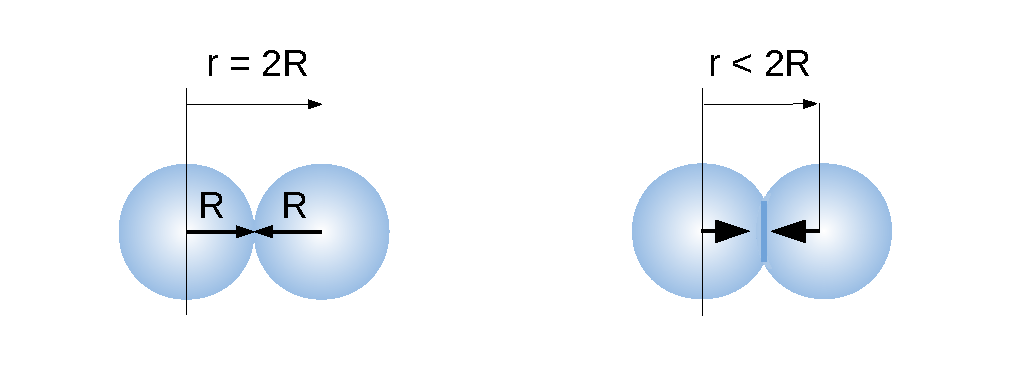
\includegraphics[height=3.5cm]{figs/TwoSpheres.pdf} 
    \caption{(Left) The WCA potential is a minimum at r=2R. 
             (Right) The WCA potential increases rapidly for $r<2R$.}
    \label{fig:TwoSpheres}
    \end{figure} 
    
\newpage
\section{The Theory of Freezing and Maxwell's Double Tangent Construction}

Freezing is governed by entropy, which the universe, or any closed system, 
seeks to maximize according to the second law of Thermodynamics. When the 
entropy of a pure substance in its liquid state is lower than the entropy 
that it would have in its solid state at the same temperature (necessary 
for thermal equilibrium), the same pressure (necessary for mechanical 
equilibrium), and the same chemical potential (necessary for diffusive 
equilibrium), an abrupt phase transition occurs, that is, the liquid freezes 
forming a crystalline structure. The particular crystalline structure and 
density that result are affected by the interatomic potential. When repulsive, 
soft sphere fluids (that are not too soft) freeze, they form lattice 
structures composed of Face Centered Cubic (FCC) crystal cells~\cite{Hansen}, 
as do hard spheres. 
This structure is what one would see by filling a cube with marbles. It 
results in the highest density achievable for hard, and nearly-hard, spheres 
that are purely repulsive. 

For pure substances, a phase transition occurs along a line on a 
Pressure-Temperature (P-T) phase diagram, such as can be seen in the phase 
diagram shown in Figure~\ref{fig:P-T_Diagram}. This phase diagram is 
representative of some arbitrary, unknown substance composed of atoms, 
or molecules which exibit both attraction and repulsion. However, since 
the atoms in a WCA fliud do not exhibit attraction there will not be a 
dividing line between the gas and liquid phases, and so the term "liquid" 
or "gas" is not used, but simply "fluid". Points along the line that 
separates the solid and the fluid phases indicate a phase transition, 
and show that the solid and the fluid both have the same temperature and 
the same pressure at a phase transistion.

%For each particular temperature, the pressure of the liquid and the 
%solid are the same at the point of transistion. 
\begin{figure}[h!]
    \centering
    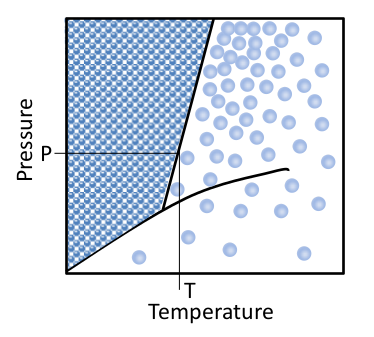
\includegraphics[height=6cm]{P-T_Diagram.png}
    \caption{Conceptual Pressure-Temperature Phase Diagram}
    \label{fig:P-T_Diagram}
  \end{figure}
The pressure can be related to the Helmholtz free energy F, which is minimized 
for a system at fixed temperature, volume and number of particles as the 
entropy of the system and its surroundings is maximized. The negative of 
the partial derivative of the Helmholtz free energy with respect to volume V 
at a fixed temperature T and number of particles N equals the pressure. 
\begin{equation}{P=-\frac{\partial{F}}{\partial{V}}\bigg|_{T,N}}\end{equation}
\noindent Dividing both the Helmholtz free energy and the volume by the 
number of particles, the partial derivative of the Helmholtz free energy 
with respect to volume becomes the partial derivative of the Helmholtz 
free energy per atom, $f$,  with respect to the inverse number density. 
\begin{equation}{P=-\frac{\partial{\frac{F}{N}}}{\partial{\frac{V}{N}}}\bigg|_{T,N} = -\frac{\partial{f}}{\partial{\frac{1}{n}}}\bigg|_{T,N}}\end{equation} Thus, the pressure corresponds to the slope of the curve on a plot of the Helmholtz free energy per atom versus the inverse density at fixed temperature. 

%In a process called Maxwell's Double Tangent construction, two curves are 
%used to find the densities of the liquid and the solid at the point of transistion. 
%Figure \ref{fig:MaxwellDT} shows a curve for the liquid, and a curve for 
%the solid both at a fixed temperature. Since the pressure of the liquid 
%is the same as the pressure of the solid at the point of transistion, the 
%density of the liquid and the density of the solid at the point of freezing 
%can be found from identifying the inverse densties at which the tangents 
%to each curve have the same slope.%
Two such curves are shown in Figure~\ref{fig:MaxwellDT}, one for the liquid 
and one for the solid at a fixed temperature. The slope of the curves is 
related to the pressure. Since the pressure of the 
liquid is the same as the pressure of the solid at the point of transistion, 
the density of the liquid and the density of the solid at the point of 
freezing can be found from identifying the inverse densties at which the 
tangents to each curve have the same slope. This process is called 
Maxwell's Double Tangent Construction. 

\begin{figure}[h!]
    \centering
     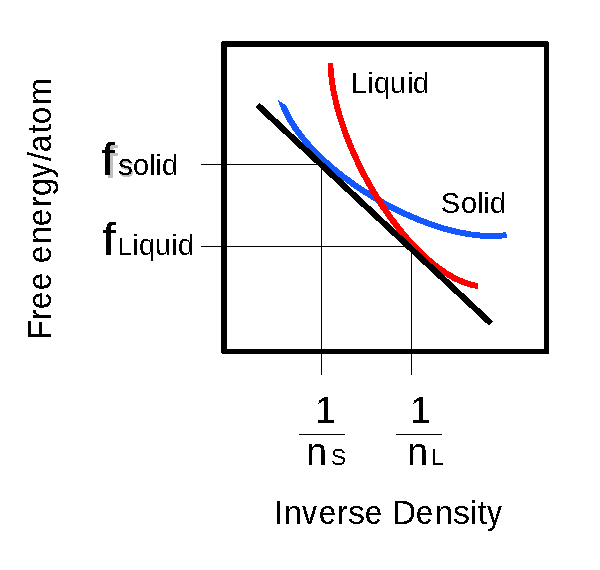
\includegraphics[height=8cm]{figs/MaxwellDTC-Fig1.pdf}
     % FIXME\includegraphics[height=7cm]{plot-pressure_Fig1.pdf}
    \caption{Identifying densities at the solid-liquid transition using 
    Maxwell's Double Tangent Construction}
    \label{fig:MaxwellDT}
  \end{figure}

To facilitate finding the pressure at the phase transition, 
%, which occurs at the points which have the same slope,
it is helpful to consider the Gibbs free energy given by G=F+PV. 
Rearranging the terms and dividing by N gives an  expression for the 
Helmholtz free energy per atom $f$ in terms of the Gibbs free energy 
per atom  $g$ (which is also the chemical potential):  
%From the Gibbs free energy an expression can be derived which relates  ....: 

%\begin{displaymath}{F=-PV+G}\end{displaymath} 
\begin{align}{\frac{F}{N}=-P\frac{V}{N}+\frac{G}{N}}\end{align} 
\begin{align}{f=-P\frac{1}{n}+g}\end{align}
This equation has the form of a line:
\begin{align}{y=mx+y_o}\end{align}
%\begin{displaymath}{G_1=G_2}\end{displaymath} 
%\begin{displaymath}{F_1+PV_1=F_2+PV_2}\end{displaymath} 
%\begin{displaymath}{\frac{F_1}{N}+P\frac{V_1}{N}=\frac{F_2}{N}+P\frac{V_2}{N}}\end{displaymath} 
and describes the black line shown in Figure~\ref{fig:MaxwellDT} with the 
pressure given by the negative of the slope of the line, and the Gibb's 
free energy per atom given by the y-intercept. 
At the point of phase transition the chemical potential of the liquid is 
the same as the chemical potential of the solid.
\begin{align}{g_L=g_S}\end{align} 
\begin{align}{f_L+P\frac{1}{n_L}=f_S+P\frac{1}{n_S}}\end{align}

The pressure at the transistion point can be obtained from the point of 
intersection that occurs when the Gibbs free energy per atom is plotted 
against the pressure for both the liquid and the solid at fixed temperature, 
as shown in Figure~\ref{fig:GibbsvsP}. These curves are constructed from 
the slope and cooresponding y-intercept data collected from lines tangent 
along the curves on the the Helmholtz free energy per atom verses inverse 
density plots (like that of Figure~\ref{fig:MaxwellDT}) for both the 
liquid and the solid at a given temperature. 
\begin{figure}[h!]
    \centering
     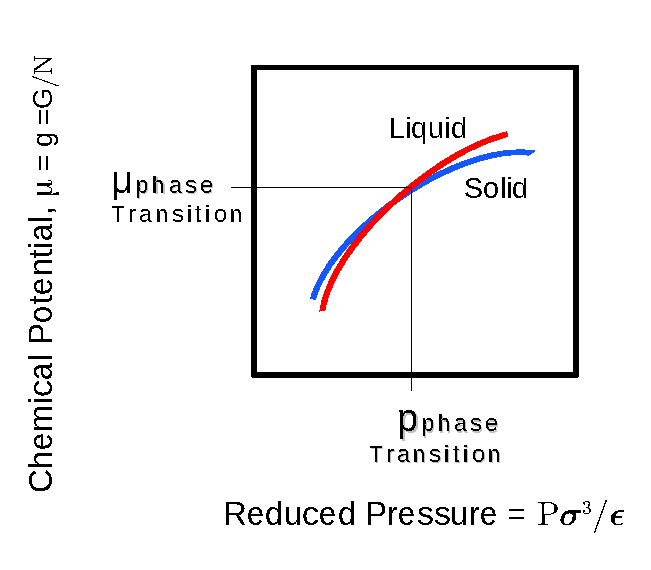
\includegraphics[height=8cm]{figs/MaxwellDTC-Fig2.pdf}
     %\includegraphics[height=7cm]{plot-pressure_Fig2.pdf}
    \caption{Pressure is found at point of intersection which occurs when $g_L=g_S$}
    \label{fig:GibbsvsP}
  \end{figure}
%CURVE FITTING! - put in methods/analysis

Once the pressure is known for the transition point, the density of the 
liquid at the transition point can be found from a plot of the pressure 
versus the inverse of the density for the liquid. The density of the solid 
at the transition point can be found the same way, as shown in Figure 
\ref{fig:Pvsinvn}. A Temperature-Density (T-n) phase diagram, such as 
that in Figure \ref{fig:T-n_Diagram}, can be generated by repeating this 
procedure for various temperatures. 
%The lowest density the crystal exhibts and the highest density the fluid 
%exhibits at the phase transistion can then be identified for each temperature.  

\begin{figure}[h!]
    \centering
    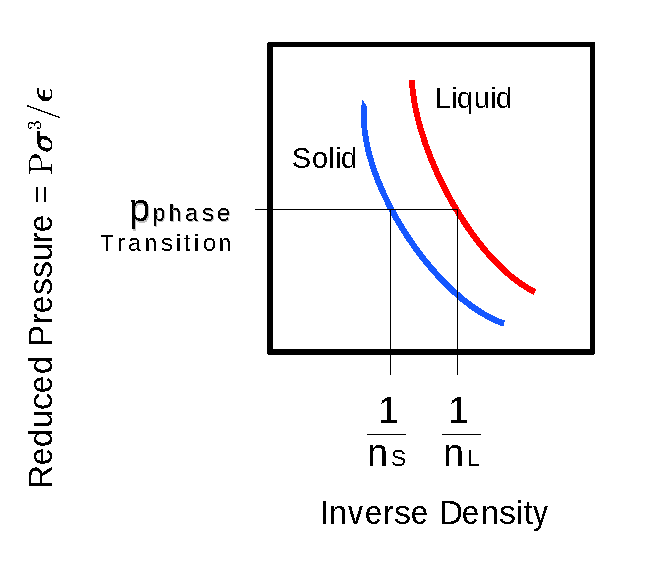
\includegraphics[height=8cm]{figs/MaxwellDTC-Fig3.pdf}
    % \includegraphics[height=7cm]{plot-pressure_Fig3.pdf}
    \caption{The liquid and solid densities at the point of transistion are 
    found from a plot of pressure vs inverse denisty for both the liquid and the solid.}
    \label{fig:Pvsinvn}
  \end{figure}

\begin{figure}[h!]
    \centering
    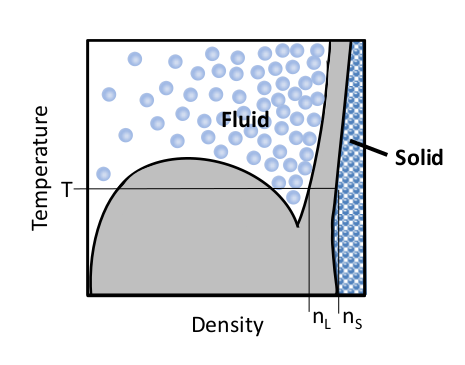
\includegraphics[height=6cm]{T-n_Diagram.png}
    \caption{Conceptual Temperature-Density Phase Diagram used to identify 
    the number densities of the liquid and the solid during a phase 
    transistion. The gray region is where the liquid and the solid coexist, 
    and are therefore not pure states.}
    \label{fig:T-n_Diagram}
  \end{figure} 
%One way of implementing this practically is to determine what the Helmholtz 
%free energy would be for both the liquid and solid phases at a particular 
%temperature and density. Whichever phase has the lower Helmholtz free 
%energy will be the phase that the substance will be in. 

\section{Classical Density Functional Theory (cDFT)}

The key idea behind classical Density Functional Theory (cDFT) is that 
free energy can be written as a functional (a function of a function) of 
a number density profile $n(\vec{r})$ which describes the way the number 
density, or atoms per volume, varies spatially on average. 
\begin{displaymath}{f[n(}\vec{r}{)]}\end{displaymath}
This, coupled with the fact that the free energy of a system tends toward 
a minimum at equilibrium means that the equilibrium free energy of the 
system ${f_{equil}}{[}\rho{(}\vec{r}{)]}$, and its corresponding equilibrium 
number density profile $\rho{(}\vec{r}{)}$, can be found simply by varying 
$n(\vec{r})$ through all possible spatial profiles until the free energy 
is minimized~\cite{MoritaDFT}. 

\begin{displaymath}{f[n(}\vec{r}{)]}\rightarrow{f_{equil}}{[}\rho{(}\vec{r}{)]}  \mbox{ as $f$ is minimized} \end{displaymath}
\begin{displaymath}{\mbox{where }  n(\vec{r})=\rho{(}\vec{r})  \mbox{ at equilibrium}}\end{displaymath}

%The reason this works is because cDFT satisfies the conditions of the 
%variational principle, the same mathematical principle used to determine 
%that the shortest distance between two points is a straight line by 
%varying the path between the two points until the distance is minimized.

A description of cDFT often begins with considering the Grand Free 
Energy defined as
\begin{equation}\Phi=F-\mu{N}\end{equation}
%\begin{equation}\int\frac{N}{V}\frac{V_{ext}}{N}dV\end{equation}
which can then be expressed in terms of a varrying number density 
profile $n(\vec r)$
%\begin{equation}\Phi=F-\int n(\vec{r})\phi{(\vec r)}d\vec{r} +\int n(\vec{r})\phi{(\vec r)}d\vec{r}-\mu{N}\end{equation}
\begin{equation}\label{GrandFE}\Phi= F_{int} +\int n(\vec{r})\phi{(\vec r)}d\vec{r}-\mu\int n(\vec r)d\vec{r}\end{equation}
where $\phi=\frac{V_{ext}}{N}$ 
is the externally 
applied potential energy $V_{ext}(\vec r)$ per particle, 
and the Helmholtz free energy is expressed as
\begin{equation}F = F_{int} + \int n(\vec{r})\phi{(\vec r)}d\vec{r}\end{equation}  
%If $\mu=0$ and $V_{ext}=0$, then the Grand free energy $\Phi$ reduces 
%to the Helmholz free energy $F$. %The second and third terms in Eq~\ref{GrandFE} 
%are both functionals of $n(\vec{r})$, so it remains to show that $F$, and 
%thus $\Phi$, is a functional of $n(\vec{r})$.

The Grand free energy is applicable to systems with a varying number of 
particles and fixed chemical potential, temperature and volume. But in 
this paper a system with a fixed temperature, volume, and number of 
particles will be of interest in which case
\begin{equation}\int n(\vec r)d\vec{r}=N\end{equation}
and so 
\begin{equation}\label{GrandFE}\Phi_{constrained}= F[n(\vec r)]-\mu N\end{equation}
The dependence on $n(\vec r)$ is now only present in the expression for 
the Helmholtz free energy, and so it is the Helmholtz energy as a functional 
of the number density profile $F[n(\vec r)]$ that is minimized at equilibrium. 
%In this paper a system with a fixed temperature, volume, and number of 
%particles will be examined in which case it is the Helmholtz energy as a 
%functional of the number density profile $F[n(\vec r)]$ that is of interest. 
More specifically, in this paper, the Helmholtz free energy per particle, 
or atom,  $f_N=\frac{F}{N}$ will be minimized which is given by
\begin{equation}f_N=\frac{U}{N}-\frac{TS}{N}\end{equation}
with differential
\begin{equation}\label{usetoshowmin}df_N=d\left(\frac{U}{N}\right)-d\left(\frac{TS}{N}\right)\end{equation}
%\begin{equation}df_N=d\left(\frac{U}{N}\right)-\frac{T}{N}dS-\frac{S}{N}dT-TS d\left(\frac{1}{N}\right)\end{equation}
\begin{equation}df_N=-\frac{S}{N}dT-\frac{P}{N}dV-PVd\left(\frac{1}{N}\right)\end{equation}
This result shows that the natural variables of the Helmholtz free energy 
per particle $f_N$ are temperature, volume and one over the number of 
particles, which in turn also holds the number density $n=\frac{V}{N}$ fixed. 
%Thus, the Helmholtz free energy will be minimized in a system that has 
%a temperature, volume, and number of particles that are fixed.
%\begin{equation}f_N(T,V, \frac{1}{N})\mbox{~~~~or~~~~}f_V(T,n)\end{equation}
\begin{equation}f_N(T,V, \frac{1}{N})\end{equation}
 
The minimization can be illustrated by considering that according to the 
second law of thermodynamics, a system that is not in equilibrium will 
exprience spontanteous processes that increase the total entropy of a 
system and its surroundings until equilibrium is reached, 
$\Delta{S}_{System + Surroundings} \geq 0$. Here ``surroundings" means 
the entire universe minus the system. This, together with the conservation 
of energy (the first law of thermodynamics) which says that energy lost 
(or gained) by the system is gained (or lost) by the surroundings 
$\Delta{U}_{System}=-\Delta{U}_{Surroundings}$, gives the result that 
changes in the free energy will be negative for spontaneous processes 
when the natural variables of the free energy are held fixed~\cite{schroeder}. 
A general proof of minimization 
can be found in Theory of Simple Fluids by Hansen and McDonald~\cite{Hansen}.

The Helmholtz free energy can be written as
\begin{equation}{F=-k_{B}T\ln(Z)}\end{equation}
which results from equating the expressions for the Helmholtz free energy 
from thermodynamics to those of statistical mechanics. The paritian function 
Z is integrated over all of phase space for N identical particles each with 
a momentum $\vec{p}$ and a position $\vec{r}$ is given by
\begin{equation}{Z=}\frac{1}{N!}\frac{1}{h^{3N}}\int{...}\int{dPdQ}~e^\frac{-H(\vec{p}_1,\vec{p}_2,...\vec{p}_N,\vec{r}_1, \vec{r}_2,...\vec{r}_N)}{k_BT}\end{equation}
\begin{displaymath}{dP=d\vec{p}_1d\vec{p}_2...d\vec{p}_N \mbox{~~~~where~~~~} d\vec{p}=dp_xdp_ydp_z}\end{displaymath}
\begin{displaymath}{dQ=d\vec{r}_1d\vec{r}_2...d\vec{r}_N \mbox{~~~~where~~~~} d\vec{r}=dxdydz\mbox{~~~~}}\end{displaymath}

Breaking the Hamiltonian, H into its component energies
\begin{equation}{H = KE + V + V_{ext} = \sum_{i=1}^N\left(\frac{|\vec{p}_i|^2}{2m}\right)+V(\vec{r}_1,\vec{r}_2,{...},\vec{r}_N)+V_{ext}(\vec{r}_1,\vec{r}_2,{...},\vec{r}_N)}\end{equation}
where the translational kinetic energy of the N atoms is given by 
\begin{displaymath}{\sum_{i=1}^N\left(\frac{|\vec{p}_i|^2}{2m}\right)}\end{displaymath}
the potential energy of the total interaction of each atom with the other 
N-1 atoms is given by
\begin{displaymath}{V(\vec{r}_1,\vec{r}_2,{...},\vec{r}_N)}\end{displaymath} 
and \begin{displaymath}{V_{ext}(\vec{r}_1,\vec{r}_2,{...},\vec{r}_N)}\end{displaymath} 
is an externally applied potential that varies spatially, such that its 
effects on each atom depend on the atom's position. Often $V_{ext}$ is 
set to zero, as it is in this paper. 

Noting that the kinetic energy depends only on momentum while the total 
interatomic and external potential energies depend only on position, 
the integral in equation (8) can be separated into two parts 
\begin{equation}{Z=\frac{1}{N!}\frac{1}{h^{3N}}\int...\int{dP}~e^\frac{-(\frac{|\vec{p}_1|^2}{2m}+\frac{|\vec{p}_2|^2}{2m}+...\frac{|\vec{p}_N|^2}{2m})}{k_BT}\int...\int{dQ}~e^\frac{-V(\vec{r}_1,\vec{r}_2,{...},\vec{r}_N)-V_{ext}(\vec{r}_1,\vec{r}_2,{...},\vec{r}_N)}{k_BT}}\end{equation}  Multiplying by $\frac{V^N}{V^N}$ where V is the real space volume satisfying \begin{equation}{V^N=}\int{...}\int{dQ}\end{equation} 
%the equation can be written
%\begin{equation}{Z=\left(V^N\frac{1}{N!}\frac{1}{h^{3N}}\int{...}\int{dP}e^\frac{-(\frac{|\vec{p}_2|^2}{2m}+ \frac{|\vec{p}_2|^2}{2m}+...\frac{|\vec{p}_N|^2}{2m})}{k_BT}\right)\left(\frac{1}{V^N}\int{...}\int{dQ}e^\frac{-V(\vec{r}_1,\vec{r}_2,{...},\vec{r}_N)-V_{ext}(\vec{r}_1,\vec{r}_2,{...},\vec{r}_N)}{k_BT}\right)}\end{equation}  
the partitian function can be expressed as
\begin{equation}\label{Zmultiply}{Z=Z_{ideal}Z_{excess}}\end{equation}
where
\begin{equation}{Z_{ideal}=V^N\frac{1}{N!}\frac{1}{h^{3N}}\int{...}\int{dP}~e^\frac{-(\frac{|\vec{p}_1|^2}{2m}+ \frac{|\vec{p}_2|^2}{2m}+...\frac{|\vec{p}_N|^2}{2m})}{k_BT}}\end{equation}
\begin{equation}{Z_{excess}=\frac{1}{V^N}\int{...}\int{dQ}~e^\frac{-V(\vec{r}_1,\vec{r}_2,{...},\vec{r}_N)-V_{ext}(\vec{r}_1,\vec{r}_2,{...},\vec{r}_N )}{k_BT}}\end{equation} The ideal partitian function $Z_{ideal}$ is associated with an ideal gas which exhibits no interaction between the atoms - a condition approached by a gas at low density where the atoms rarely encounter one another. The excess partitian function $Z_{excess}$ accounts for the interaction of all the atoms according to their interatomic potential. The free energy can also be broken into two parts using Equation~\ref{Zmultiply} giving
%\begin{equation}{F=-k_{B}T\ln(Z)}\end{equation}
\begin{equation}{F=-k_{B}T\ln(Z_{ideal}Z_{excess})}\end{equation}
\begin{equation}{F=-k_{B}T\ln(Z_{ideal})-k_{B}T\ln(Z_{excess})}\end{equation}
\begin{equation}{F=F_{ideal} + F_{excess}}\end{equation} 

The ideal Helmholtz free energy is
\begin{displaymath}{F_{ideal}=-k_BT\ln{\left(V^N\frac{1}{N!}\frac{1}{h^{3N}}\int{...}\int{dP}~e^\frac{-(\frac{|\vec{p}_1|^2}{2m}+ \frac{|\vec{p}_2|^2}{2m}+...\frac{|\vec{p}_N|^2}{2m})}{k_BT}\right)}}\end{displaymath}  

\begin{equation}{\label{Fidealmultipleint}}{=-k_BT\ln\left(V^N\frac{1}{N!}\frac{1}{h^{3}}\int{d\vec{p}_1}~e^\frac{-\frac{|\vec{p}_1|^2}{2m}}{k_BT}\frac{1}{h^{3}}\int{d\vec{p}_2}~e^\frac{-\frac{|\vec{p}_2|^2}{2m}}{k_BT}{...}\frac{1}{h^{3}}\int{d\vec{p}_N}~e^\frac{-\frac{|\vec{p}_N|^2}{2m}}{k_BT}\right)}\end{equation}
These integrals can conveniently be written in terms of the DeBroglie 
wavelength $\Lambda$, or the quantum volume $\text{n}_\text{Q}$
\begin{equation}{\frac{1}{h^{3}}\int{d\vec{p}}~e^\frac{-\frac{|\vec{p}|^2}{2m}}{k_BT}=\left(\sqrt{\frac{k_BTm}{2\pi\hbar^2}}\right)^3=\frac{1}{\Lambda^{3}}}=\text{n}_\text{Q}\end{equation} 
where \begin{equation}{\Lambda =\sqrt{\frac{2\pi\hbar^2}{k_BTm}}}\end{equation} 
Rewriting Equation~\ref{Fidealmultipleint} in terms of $\Lambda$ gives
\begin{equation}{F_{ideal}= -k_BT[\ln(V^N)-\ln(N!) - \ln(\Lambda^{3N})]}\end{equation}
Using Stirling's approximation \begin{equation}{\ln(N!)=N\ln{N}-N}\end{equation} 
this becomes
\begin{equation}{F_{ideal}= k_BT[N\ln(\frac{N\Lambda^{3}}{V}{)-N}]}\end{equation} 
Rewriting the equation in terms of the number density $n=\frac{N}{V}$, 
and the quantum volume, $\text{n}_\text{Q}$ gives
\begin{equation}{F_{ideal}= k_BT\left[\frac{N}{V}\ln{\left(\frac{N}{V}\frac{1}{\text{n}_\text{Q}}\right)}-\frac{N}{V}\right]}V\end{equation}
\begin{equation}\label{eq:Fideal}{F_{ideal}= k_BT[n\ln(n/\text{n}_\text{Q})-n]V}\end{equation}   
For a spatially varying number density, the ideal free energy in 
Equation~\ref{eq:Fideal} becomes
\begin{equation}\label{eq:Fideal-n(r)}{F_{ideal}[n(\vec{r})]= k_BT\int_{Vol}[n(\vec{r})\ln(n(\vec{r})/\text{n}_\text{Q})-n(\vec{r})]d\vec{r}}\end{equation} 

Now consider the excess free energy which is written most generally as
\begin{equation}\label{Fexcess-mostgeneral}{F_{excess}= -k_BT\ln{\left(\frac{1}{V^N}\int{...}\int{dQ}~e^\frac{-V(\vec{r}_1, \vec{r}_2,...\vec{r}_N)-V_{ext}(\vec{r}_1, \vec{r}_2,...\vec{r}_N)}{k_BT}\right)}}\end{equation} 
This integral can be greatly simplified if it can be assumed that the 
potential energy $V(\vec{r_1},\vec{r_2},...\vec{r_N})$ is a sum of the 
potential energies between pairs of atoms, where each atom is paired in 
turn with each of the other atoms in the system. In this case 
$V(\vec{r}_1, \vec{r}_2,...\vec{r}_N)$ becomes 
\begin{equation}{V(\vec{r_1},\vec{r_2},...\vec{r_N})=\frac{1}{2}\sum^N_i\sum^N_{j\neq{i}}V_{ij}(\vec{r_i},\vec{r_j})}\end{equation} 
%\begin{displaymath}{=V_{12}(\vec{r_1},\vec{r_2})+V_{13}(\vec{r_1},\vec{r_3}) + V_{14}(\vec{r_1},\vec{r_4}) + ...}\end{displaymath}
%\begin{displaymath}{+ V_{23}(\vec{r_2},\vec{r_3})+V_{24}(\vec{r_2},\vec{r_4})+V_{25}(\vec{r_2},\vec{r_5})+ ...}\end{displaymath} 
%\begin{displaymath}{+ V_{34}(\vec{r_3},\vec{r_4})+V_{35}(\vec{r_3},\vec{r_5})+V_{36}(\vec{r_3},\vec{r_6})+...}\end{displaymath}
Using this potential, and setting the external potential 
$V_{ext}(\vec{r}_1, \vec{r}_2,...\vec{r}_N)$ to zero, the exponent in 
Equation~\ref{Fexcess-mostgeneral} becomes

\begin{displaymath}{e^{-\frac{\frac{1}{2}\sum^N_i\sum^N_{j\neq{i}}V_{ij}(\vec{r_i},\vec{r_j})}{k_BT}}=e^{\frac{-V_{12}(\vec{r_1},\vec{r_2})}{k_BT}}e^{-\frac{V_{13}(\vec{r_1},\vec{r_3})}{k_BT}}e^{-\frac{V_{14}(\vec{r_1},\vec{r_4})}{k_BT}}...}\end{displaymath}    \begin{equation}{\approx-(1+f_{12})(1+f_{13})(1+f_{14})...}\end{equation}
where each exponential term is simplified by a Taylor expansion $e^x\approx{1+x}$. 
%\begin{equation}{\exp^{-V_{ij}(\vec{r_i},\vec{r_j})}\approx 1+f_{ij}(\vec{r_i},\vec{r_j})}\end{equation}%    
%$\exp^x=1+x+\frac{x^2}{2!}+\frac{x^3}{3!}...$.%  
The function $f_{ij}$ is called a Mayer function, and is given by
\begin{equation}\label{eq:mayerfunction}{f_{ij}(\vec{r_i},\vec{r_j})=e^{-\frac{V_{ij}(\vec{r_i},\vec{r_j})}{k_BT}}-1}\end{equation} 
Multiplying the Mayer function terms, the excess free energy can be written as
\begin{equation}\label{eq:Fexcess-simplified}{F_{excess}=-k_BT\ln{\left(\frac{1}{V^N}\int{...}\int{dQ}\left[1 + \sum{f_{ij}} + \sum{f_{ij}f_{kl}} +\sum{f_{ij}f_{kl}f_{mn}} +... \right]\right)  }}\end{equation}

  \begin{figure}[h!]
    \centering
    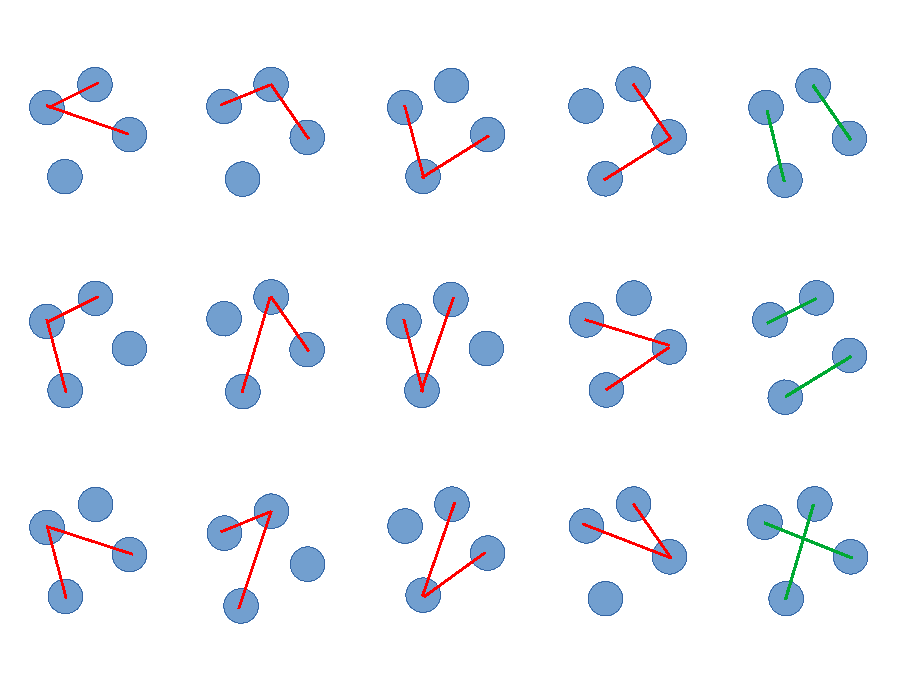
\includegraphics[height=7cm]{figs/diagrammic.pdf}
    \caption{Two-pair Interactions $f_{ij}f_{kl}$ for N=4 atoms. Interations 
    between individual pairs of atoms are shown in green. Interactions 
    between pairs of atoms with an atom shared in common are shown in red. 
    At low densities only the interactions shown in green are considered, 
    since atoms are not likely to be clustered.}
    \label{fig:diagrammic}
  \end{figure}

At low densities, it is not likely to find two or more atoms in close 
proximity, and so only interactions between individual pairs of spheres, 
such as those shown in green in Figure~\ref{fig:diagrammic}, are considered.
Each pair can then be described by a function of the distance between the 
two atoms in the pair. 
%Making a change of variables $\vec{r}=\vec{r}_i-\vec{r}_j $ for each pair we get 
%\begin{equation}f_{ij}(\vec{r_i}-\vec{r_j})=f(\vec{r})=e^{-\frac{V(\vec{r})}{k_BT}}-1\end{equation} 
With a careful counting of the resulting number of such pairs, the excess 
free energy can then be written~\cite{schroeder} as
%\begin{equation}{F_{excess}=-k_BT\ln\left(1+\frac{1}{2}\frac{N^2}{V}\int{f(r)}{d\vec{r}}+\frac{1}{2}\left(\frac{1}{2}\frac{N^2}{V}\int{f(r)}{d\vec{r}}\right)^2+ ...\right)}\end{equation}
%where in the thermodynamic limit (large N), $N-1, N-2, ...\approx{N}$. 
%Written in terms of an exponential $e^x=1+x+\frac{x^2}{2!}+\frac{x^3}{3!}+ ...$ 
%for a homogeneous density n=$\frac{N}{V}$ this becomes
%\begin{equation}{F_{excess}=-k_BT\ln{\left(e^{\frac{1}{2}\frac{N^2}{V}\int{f(r)}{d\vec{r}}}\right)}}\end{equation} 
%Thus the free excess energy per atom in the low-density limit is given by 
\begin{equation}\label{eq:Fexcess}{\frac{F_{excess}}{N}=k_BTn\left(-\frac{1}{2}\int{f(r)}{d\vec{r}}\right)}\end{equation} 
in the thermodynamic limit of large N 
where the quantity in parenthesis can be recognized 
as the second virial expanision coefficient typically called $B_2$. 
%where $x=\frac{1}{2}\frac{N(N-1)}{V^{2}}\int{...}\int{dQ}{f_{12}}$.% 
It is important that the expression for the excess Helmholtz free energy 
correctly reduces to this result in the low-density limit. 
%Although we will not be restricting ourselves to the low-density limit, 
%it is important that the theory we use correctly reduces to this same 
%result in the low-density limit. 
Outside of the low density limit, it is quite difficult to evaluate the 
excess Helmholtz free energy given in Equation~\ref{eq:Fexcess-simplified}. 

%Equations~\ref{eq:Fideal} and \ref{eq:Fexcess} show that the Helmholtz free energy 
%\begin{equation}{F=F_{ideal} + F_{excess}}\end{equation} 
%is a function of the number density n. For a spatially varying number density, 
%as would be expected for a crystal, the free energy becomes a functional of 
%the number density profile $n(\vec{r})$.  

%According to classical Density Functional Theory, 

%A number density profile is a time-invariant average 
%of the spacial distribution of the particles that make up the fluid, and
%There will be one, and only one 
%that minimizes the Helmholtz free energy.
%The minimum free energy, 
%is the value of the Helmholtz free energy that
%the system will have when it is in equilibrium at that temperature, 
%and its corresponding number density profile 
%are the equilibrium values the system will have at that temperature.
%is the equilibrium number density profile. 
%
Once an expression for the Helmholtz free energy as a functional of the
number density profile $n(\vec r)$ is formed then, according to classical 
Density Functional Theory, the equilibrium value of the 
Helmholtz energy, and its cooresonding equilibrium density profile can be
found by varying the number density profile
%can be varied 
through all possible configurations at some fixed temperature
until the free energy is minimized.  
In this section 
%To form the functional for the Helmholtz free energy, expressions for 
a functional for the Helmholtz free energy was formed by finding 
general expressions for the ideal and the excess portions of the free 
energy, and adding them together.
\begin{equation}{F[n(\vec{r})]=F_{ideal}[n(\vec{r})] + F_{excess}[n(\vec{r})]}\end{equation}
The functional for the ideal portion of the Helmholtz free energy is given by 
Equation~\ref{eq:Fideal-n(r)}, and a functional for the excess portion of the Helmholtz 
free energy is given in Equation~\ref{eq:Fexcess-simplified}. The specific 
form for the excess Helmholtz free energy depends on the particular 
fluid being modeled as defined by the  
interatomic potential energy V(r) between the spheres, which can make
forming an expression difficult. In this paper, Soft Fundamental Measure
Theory will be used to form an epxression for the excess Helmholtz free 
energy, as explained in the next section.

\section{Soft Fundamental Measure Theory (SFMT)}
In order to apply classical Density Functional Theory to a system that has
a fixed temperature, volume, and nubmer of particles, a functional for 
the Helmholtz free energy must first be formed. An expression for the ideal 
portion of the Helmnoltz free energy is given by Equation~\ref{eq:Fideal-n(r)}, 
but forming an expression for the excess Helmholtz free
energy from Equation~\ref{eq:Fexcess-simplified} for the particular fluid 
being modeled can be challenging. 
Soft Fundamental Measure Theory (SFMT) is a method for forming an 
expression for the excess Helmholtz free energy of a Soft-sphere fluid
that does not depend on  explicitly taking into account the interaction 
that each sphere with every other sphere in the fluid as required by 
Equation~\ref{eq:Fexcess-simplified}. In the next chapter on methods, we
will use an SFMT functional that we adapt to fit the soft-sphere WCA fluid.

SFMT is an extension of Fundamental Measure Theory (FMT)
that was developed for the Hard-sphere fluid, and which can be derived from
Scaled Particle Theory (SPT).  
%For the Hard Sphere fluid, there is another way to form an expression for 
%the excess Helmholtz free energy in terms of a homogeneous number density 
%and, that is to use Scaled Particle Theory (SPT)~\cite{ReissSPT}.
Scaled Particle Theory seeks a general expression for the excess chemical 
potential of a homogeneous Hard Sphere fluid which can then be integrated 
to find the excess Helmholtz free energy according to the relation
%\begin{equation}F_{ex}=\int{\mu_{ex}dN}\end{equation}
%\begin{equation}\mu_{ex}=\frac{\partial{F_{ex}}}{\partial{N}}\bigg|_{T,V}\end{equation}
\begin{equation}\mu_{ex}=\frac{\partial{F_{ex}}}{\partial{N}}\bigg|_{T,V}{~~~~~}\rightarrow{~~~~~}F_{ex}=\int{\mu_{ex}dN}\end{equation}
It is an extension of the work done by Widom who showed that the excess 
chemical potential of a homogenesous fluid corredsponds to the reversible 
work of inserting a sphere of radius R into a fluid consisting of hard 
spheres of radius R. 
\begin{align}
	\mu_{ex}=W_{rev}(R){~~~~}\text{work to insert a hard sphere of radius R}
\end{align}
Widom's result was obtained by considering the difference 
in the excess Helmholtz free energy when one atom is added to an otherwise 
closed system. He showed that the excess chemcial potential is related to 
the ensemble average of the Boltzman factor for the potential energy 
difference $V_{diff}$ between a system with N atoms and one with N+1 atoms. 
The resulting equation, shown below, is known as Widom's Insertion 
Formula~\cite{Hansen}.
%\begin{displaymath}\mu_{ex}=\frac{\partial{F_{ex}}}{\partial{N}}\bigg|_{T,V}{~~~~~~}\end{displaymath}
\begin{equation}\mu_{ex}=\frac{F_{ex}(N+1)-F_{ex}(N)}{\Delta{N}}\bigg|_{T,V}\end{equation}
\begin{equation}\label{widoms-insertion-formula}{~}=-k_BT\ln\left(<e^{-\beta{V_{diff}}}>\right)\end{equation}

The quantity $<e^{-\beta{V_{diff}}}>$ can be evaluated by considering
that at each point in the fluid, there is a probability that 
a hard sphere of radius R has space available to exist at that point
without overlapping with other spheres, or it does not, as shown in 
Figure~\ref{fig:p_overlap}. 
\begin{figure}[h!]
    \centering
    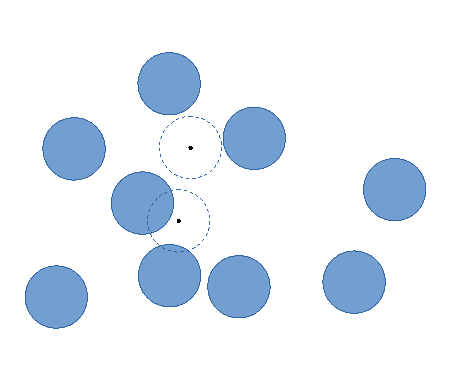
\includegraphics[height=7cm]{figs/P_overlap.pdf}
    \caption{No energy is needed to place a sphere at a position where 
    there is no overlap such as shown by the black dot at the center of 
    the dotted region near the top. But it is not possible to place a 
    sphere at a position where an overlap occurs.}
    \label{fig:p_overlap}
  \end{figure}
Widom's Insertion formula Equation~\ref{widoms-insertion-formula}, then becomes
\begin{align} 
	\mu_{ex} &= -k_BT\ln\left(e^{-\beta{V_{diff}}}+1\right)  \\
	         &= V_{diff} \\
             &= W_{rev}(R)  \label{workrev}
\end{align}
The quantity $<e^{-\beta{V_{diff}}}>$ can also be evaluated by considering
that it takes no energy for a hard sphere to be placed at a point
in the fluid where it does not overlap with any other spheres 
($V_{diff}=0$), but it would require infinite energy ($V_{diff}=\infty$)
to place a sphere where it would overlap another sphere, as described 
in Figure~\ref{fig:p_overlap}.
In this case Equation~\ref{widoms-insertion-formula} becomes
%\begin{equation}\mu_{excess}=-k_BT\ln(1-n\frac{4\pi}{3}R_{cavity}^3) &  \mbox{for} & R_{\cavity}=R\end{equation}
\begin{align} \label{muexcess}
  \mu_{excess}(R_{cavity}=R)=-k_BT\ln(1-n\frac{4\pi}{3}R^3) 
\end{align}
where the radius of the cavity $R_{cavity}$ equals the radius of a hard sphere R,
and $nV_{Sphere}$ is the probability that a sphere cannot be placed at
some random point in the homogeneous fluid of number density, $n$, without
overlapping with another sphere. Combining  Equations~\ref{workrev} and \ref{muexcess} gives
\begin{align}
  W_{rev}(R_{cavity}=R)=-k_BT\ln(1-n\frac{4\pi}{3}R^3) 
\end{align}
%where the radius of the cavity $R_{cavity}$ is equal to the radius of a 
%hard sphere, R, and $<e^{-\beta{V_{diff}}}>$ is evaluated using the 
%probablities that the cavity is either filled or not filled~\cite{Hansen}.
%For cavities that are much larger than one of the hard spheres, 
Forming a more general result by requiring continuity of the functions, 
along with their first and second derivatives, for the reversible work
written for fluids with a cavitiy radius 
%$\operatorname{R}_{cavity}$ 
equal to, larger than, or very 
much larger than the hard sphere radius R, Scaled Partical Theory arrives 
at an expression~\cite{Hansen} for the excess Helmholtz free energy of 
a homogeneous Hard-Sphere fluid in terms of the packing fraction $\eta$ 
\begin{equation}\label{Fexcess-SPT}{\frac{\beta{F_{excess}}}{N}=-ln(1-\eta)+\frac{3\eta}{1-\eta}+\frac{3{\eta}^2}{2(1-\eta)^2}}\end{equation} 
where
\begin{equation}{\eta = \frac{\mbox{Volume occupied by the spheres}}{\mbox{Total Volume}}}\end{equation}
\begin{equation}{\eta = \frac{N\frac{4}{3}\pi{R^3}}{V}}\end{equation}


%for the excess Helmholtz 
%free energy obtained from Scaled Partical Theory for a homogeneous 
%Hard-Sphere fluid, 
Fundamental Measure Theory~\cite{rosenfeld1989} (FMT) 
can be constructed from Equation~\ref{Fexcess-SPT}~\cite{santos2012phi3},  
and provides an expression for the excess Helmholtz free energy of an 
inhomogeneous 
Hard-Sphere fluid as a functional of the number density profile $n(\vec r)$. 
%FMT was developed for hard sphere fluids, and has been very sucessful 
%at predicting the thermodynamic properties of inhomogeneous hard sphere fluids. 
Soft Fundamental Measure Theory (SFMT), which will be used in this paper, 
is an extension of FMT and provides an expression for the excess Helmoholtz
free energy of fluids with soft potentials like that of the WCA fluid. 
It will be helpful to continue looking at FMT before addressing SFMT.

Fundamental Mearsure Theory begins by noticing that 
%\begin{equation}{\eta = \frac{NR_{3}}{V}}\end{equation}
%\begin{equation}{\eta = \left(\frac{N}{V}\right)\frac{4}{3}\pi{R^3}}\end{equation}
%\begin{equation}{\eta = n\frac{4}{3}\pi{R^3}=nR_{3}=n_{3}}\end{equation}
from Equation~\ref{Fexcess-SPT}, a quantity $G_{3}$ can be defined as follows
\begin{equation}{\eta =\left(\frac{N}{V}\right)\frac{4}{3}\pi{R^3}=nG_{3}}\end{equation}
where $G_{3}$ is the volume of a sphere. Likewise, by defining
quantities
\begin{equation}{G_{2}=4\pi{R^2}}\end{equation}
\begin{equation}{G_{1}=R}\end{equation}
\begin{equation}{G_{0}=1}\end{equation}
where $G_{2}$ is the surface area of a sphere, and $G_{1}$ is the 
radius of a sphere, Equation~\ref{Fexcess-SPT} can be written as
%reproduced by introducing a set of weighted densities $n_{i}=nG_{i}$.
\begin{equation}\label{FexfromSPTinthermsofG}{F_{excess}=k_{B}T\left(-nG_{0}ln(1-nG_{3})+\frac{nG_{1}nG_{2}}{1-nG_{3}}+\frac{nG_{2}^3}{24\pi(1-Gn_{3})^2}\right)V}\end{equation}
The quantities $G_{3}, G_{2}, G_{1},$ and $G_{0}$ are fundamental 
geometric measures of a sphere, and are what give rise to the name
Fundamental Measure Theory. Introducing a set of weighted densities $n_{i}=nG_{i}$ 
given by
%and they will prove useful by introducing a set of weighted densities 
%$n_{i}=nG_{i}$ where $n=\frac{N}{V}$. 
\begin{equation}\label{n3}{n_{3}=nG_{3}=\left(\frac{N}{V}\right)\frac{4}{3}\pi{R^3}=\eta}\end{equation}
\begin{equation}\label{n2}{n_{2}=nG_{2}=\left(\frac{N}{V}\right)4\pi{R^2}=\frac{3\eta}{R}}\end{equation}
\begin{equation}\label{n1}{n_{1}=nG_{1}=\left(\frac{N}{V}\right)R}\end{equation}
\begin{equation}\label{n0}{n_{0}=nG_{0}=\left(\frac{N}{V}\right)}\end{equation}
Equation~\ref{FexfromSPTinthermsofG} can be written as
%Writing Eq~\ref{Fexcess-SPT} in terms of the number density $n=\frac{N}{V}$
%\begin{equation}{F_{excess}=k_{B}T\left(-\frac{N}{V}ln(1-\eta)+\frac{N}{V}\frac{3\eta}{1-\eta}+\frac{N}{V}\frac{3{\eta}^2}{2(1-\eta)^2}\right)V}\end{equation}
%and using the expressions in Equations~\ref{n3} through~\ref{n0}, this becomes
\begin{align}\label{FexfromSPT}
    F_{excess}=k_{B}T\left(-n_{0}ln(1-n_{3})+\frac{n_{1}n_{2}}{1-n_{3}}+\frac{n_{2}^3}{24\pi(1-n_{3})^2}\right)V
\end{align}
which has the form 
\begin{align}
    F_{excess} = k_BT(\Phi_1+\Phi_2+\Phi_3)V
\end{align}
or for a spatially varying number density $n(\vec{r})$, 
\begin{equation}\label{eq:F_ex-n-of-r}{F_{excess}[n(\vec{r})]= k_BT\int(\Phi_1(\vec{r})+\Phi_2(\vec{r})+\Phi_3(\vec{r}{)) d}\vec{r}}\end{equation} 
where 
\begin{align}
   \Phi_1 &= -n_{0}ln(1-n_{3}) \\
   \Phi_2 &= \frac{n_{1}n_{2}}{1-n_{3}} \\
   \Phi_3 &= \frac{n_{2}^3}{24\pi(1-n_{3})^2}   \label{oldPhi3equation}
\end{align}

The quantities $n_{0},n_{1},n_{2},n_{3}$ can be considered as weighted 
densities where the weights are given by $G_{0},G_{1},G_{2},G_{3}$ respectively.
\begin{align}
    n_{i}=nG_{i}
\end{align}
These weights are valid for determining the excess free energy of a system of 
hard spheres with a homogeneous number density n. But these weights, and 
their related  weighted densities, can be written in a more general form 
allowing for their extention to a system with a spacially varying number 
density, that is, an inhomogeneous fluid. Using a backwards Heavyside step function defined as
\begin{displaymath}{\Theta(|\vec{r}|-R)=\left\{ \begin{array}{rc} 1 & 0<r \leq R \\ 0  & r>R \end{array}\right.}\end{displaymath}
the following expressions are obtained
\begin{equation}{G_{3}=\int_{Volume}{\Theta(|\vec{r}|-R)d{\vec{r}}} = \frac{4}{3}\pi{R^3}}\end{equation}
\begin{equation}{G_{2}=\int_{Volume}{\delta(|\vec{r}|-R)d{\vec{r}}} = 4\pi{R^2}}\end{equation}
%\begin{equation}{G_{1}=\frac{R_{2}}{4\pi{R}}=R}\end{equation}
\begin{equation}{G_{1}=\int_{Volume}{\frac{\delta(|\vec{r}|-R)}{r}d{\vec{r}}} = R}\end{equation}
%\begin{equation}{G_{0}=\frac{R_{2}}{4\pi{R}^2}=1}\end{equation}
\begin{equation}{G_{0}=\int_{Volume}{\frac{\delta(|\vec{r}|-R)}{r^2}d{\vec{r}}} = 1}\end{equation}
where the weighted densities can now be expressed as
%CHECK
\begin{align}
    n_{i}=\int_{Volume}{nw_{i}(r)}d{\vec{r}}
\end{align} 
or for a spatially varying number density $n(\vec{r})$,
\begin{equation}{n_i(\vec{r})=\int_{Volume}{n(\vec{r'})w_i(|\vec{r}-\vec{r'}|)d{\vec{r'}}}}\end{equation}
with weight functions
\begin{equation}\label{eq:w3}{w_{3}=\Theta(|\vec{r}|-R)}\end{equation}
\begin{equation}\label{eq:w2}{w_{2}=\delta(|\vec{r}|-R)}\end{equation}
%\begin{equation}{w_{1}=\frac{w_{2}}{4\pi{R}}}\end{equation}
\begin{equation}\label{eq:w1}{w_{1}=\frac{w_{2}}{4\pi{r}}}\end{equation}
%\begin{equation}{w_{0}=\frac{w_{2}}{4\pi{R}^2}}\end{equation}
\begin{equation}\label{eq:w0}{w_{0}=\frac{w_{2}}{4\pi{r}^2}}\end{equation}
The weight functions $w_{2}$ and $w_{3}$ have the relation
\begin{equation}\label{w2_w3_relation}{w_{3}=\int_{r}^{\infty}{w_{2}(\vec{r})dr}\mbox{~~~~or equivilantly,~~~~}-\frac{\partial{w_3(r)}}{\partial{r}}=w_2(r)}\end{equation}
which will be important to keep in tact when moving to SFMT.


The weight functions can be related to the mayer function 
\begin{align}
     f(r)=\exp^{-\frac{V(r)}{k_{B}T}}-1
\end{align} 
where r is the distance between the centers of two hard spheres, and 
$V(r)$ is the interatomic potential between two hard spheres given by 
\begin{align}
    V(r)=\left\{ \begin{array}{rc} \infty & 0<r \leq 2R \\ 0  & r>2R \end{array}\right.
\end{align}
Evaluating Equation with $V(r)$ given by Equation,  
the mayer function for a Hard-sphere fluid is found to be
\begin{equation}\label{f(r)step}{f(r)=-\Theta(|\vec{r}|-2R)}\end{equation} 
which can be written in terms of the weight functions if two 
additional vector weight functions $\vec{w_2}$ and $\vec{w_1}$ are introduced
\begin{equation}\label{eq:w_v2}{\vec{w_{2}}=w_{2}\frac{\vec{r}}{r}}\end{equation}
\begin{equation}\label{eq:w_v1}{\vec{w_{1}}=w_{1}\frac{\vec{r}}{r}}\end{equation} 
The mayor function can then be written in terms of the weight functions~\cite{Hansen}
\begin{equation}\label{mayer_deconvolution}{f(r)=-\Theta(|\vec{r}|-2R)= -2(w_3 \otimes w_0 + w_2 \otimes w_1 + \vec{w_2} \otimes \vec{w_1})}\end{equation}  

Taking the derivative of the mayer function in Eq~\ref{f(r)step} provides 
another relation that will be important to keep in tact when moving to SFMT.
\begin{align}\label{mayerder=w2convolution}
     \frac{df(r)}{dr} = w_2 \otimes w_2 = \int{w_2(r')w_2(r-r')dr'}
\end{align} 
This can easily be checked by evalating the left side for a Hard-sphere fluid as follows,
%where, for a hard sphere fluid the left side of Equation~\ref{mayerder=w2convolution} gives
\begin{displaymath}{\frac{df(r)}{dr}=\left\{ \begin{array}{rc} \frac{d}{dr}(-1)=0 & r<2R \\\frac{d}{dr}(\text{vertical line})=+\infty & r=2R \\ \frac{d}{dr}(0)=0  & r>2R \end{array}\right.}\end{displaymath}
\begin{equation}\label{mayerder}{\frac{df(r)}{dr} = \delta(r-2R)}\end{equation} 
and evaluating the right side by using the general relation for convolution which is equal to the Inverse 
Fourier Transform of a product of Fourier Transforms. 
\begin{equation}{f \otimes g = \text{I.F.T.[ F.T.}[f]\text{ x F.T.[g] }]}\end{equation} 
Taking the Fourier Transform of the weight function $w_2(r)=\delta(r-R)$ 
%\begin{equation}{w_2(r)=\delta(r-R)}\end{equation} 
gives
\begin{equation}{\text{F.T.}[w_2]=\int_{-\infty}^{\infty}\delta(r-R)e^{-ikr}dr=e^{-ikR}}\end{equation} 
and the right side of Equation~\ref{mayerder=w2convolution} becomes
\begin{equation}{w_2 \otimes w_2 = \text{I.F.T.}[e^{-ikR}e^{-ikR}]}\end{equation} 
\begin{equation}\label{w2convolution}{=\int_{-\infty}^{\infty}e^{-ik2R}e^{ikr}dk=\int_{-\infty}^{\infty}e^{ik(r-2R)}dk=\delta(r-2R)}\end{equation} 
which matches Equation~\ref{mayerder}.

Tarazona later improved upon the original FMT equations by replacing the
expression for $\Phi3$ given by Equation~\ref{oldPhi3equation} with the
more accurate expression~\cite{tarazonaphi3, santos2012phi3} 
%
%The final FMT expression for the excess Helmholtz free energy is given by
%
%Incorporating the two vector weights which 
%were added to satisfy Equation~\ref{mayer_deconvolution}, and an updated 
%expression for $\Phi_3$ developed by Tarazona~\cite{tarazonaphi3, santos2012phi3}, 
%into Equation~\ref{FexfromSPT} the excess free energy becomes
%\begin{equation}{F_{excess} = k_BT(\Phi_1+\Phi_2+\Phi_3)V}\end{equation}
%where
\begin{align}
%\Phi_1 &= -n_{0}ln(1-n_{3}) \label{eq:Phi1}\\
%\Phi_2 &= \frac{n_{1}n_{2}-\vec{n_{1}}\cdot\vec{n_{2}}}{1-n_{3}} \label{eq:Phi2} \\
\Phi_3 &= \frac{{n_2}^3-3n_2\vec{n}_{v2}\cdot\vec{n}_{v2}+\frac{9}{2}[\vec{n}_{v2}\cdot{\overleftrightarrow{n}_{m2}}\cdot{\vec{n}_{v2}}-\operatorname{Tr}({\overleftrightarrow{n}^3_{m2}})]}{24\pi(1-n_3)^2}  \label{eq:Phi3}
\end{align}
in which a tensor weight is incoporated given by
\begin{equation}\label{eq:tensorweight}{\overleftrightarrow{w}_{m2}(\vec{r})=w_2(r)\left(\frac{\vec{r}\vec{r}}{r^2}-\frac{I}{3}\right)}\end{equation} 
All the other FMT equations remain the same.

%The expression for the weighted densities can be written in a way that 
%accomodates both homogenious fluids where the number denstiy n is constant, 
%and inhomogeneous fluids where the number density becomes a function of 
%the position $n(\vec{r})$.
%\begin{equation}{n_i(\vec{r})=\int_{Volume}{n(\vec{r'})w_i(|\vec{r}-\vec{r'}|)d{\vec{r'}}}}\end{equation}
%The equatons above were derived for a uniform fluid where the number density n is constant, 
%but they can be extended for inhomogenious fluids where the number density becomes a function of r, $n(\vec{r})$.
%For a spatially varying number density $n(\vec{r})$, the excess Free 
%Energy becomes a functional of the number density profile $n(\vec{r})$ 
%\begin{equation}\label{eq:F_ex-n-of-r}{F_{excess}[n(\vec{r})]= k_BT\int(\Phi_1(\vec{r})+\Phi_2(\vec{r})+\Phi_3(\vec{r}{)) d}\vec{r}}\end{equation} 

The FMT equations developed so far have been for a Hard-sphere fluid.
All of the weight functions, the relations between them, and the equation 
for the deriviative of the mayer function, can be expressed in terms of 
$w_{2}(r)$ which, for a Hard-sphere fluid, consists of a delta function 
characteristic of hard spheres. 
Soft Fundamental Measure Theory extends FMT discussed so far to fluids 
with soft potenials by keeping the relationships between the weight 
functions the same, but replacing $w_{2}(r)$ with a weight function 
appropriate for a soft sphere potential. This is what we do to
%A new set of weight functions can then be derived for a system of soft spheres  
form a functional for the 
Weeks-Chandler-Anderson fluid as detailed in the next chapter on Methods.

\chapter{Methods}

\section{The Overall Approach}
%
%The goal of this project is to generate phase diagrams for a 
%Weeks-Chandler-Anderson model fluid using a computer program. 
%To do this we find the Helmholtz free energies that the fluid
%would have at a given temperature and density in a  
%liquid state, and in a crystalline solid state. 
%%Once the Helmholtz free energy for both the crystal and liquid states of 
%%the fluid are found for a given temperature and density, they can be 
%%compared to find the resulting state of the fluid. 
%Outside the region of 
%coexistence which exists between the liquid and crystal states, 
%the fluid will be completely in a crystalline state if the 
%crystal free energy is lower than the liquid free energy, and it will be 
%completely in a liquid state if the liquid free energy is lower than 
%the crystal free energy. Maxwell's Double Tangent Construction is used 
%to determine the actual number densities of the crystal and liquid states
%at the boundaries of the coexistance region for a given temperature, 
%and construct phase diagrams.

%%In general, if at some number density and temperature the crystal free energy 
%%is lower than the homogeneous free energy of the liquid, then the fluid will 
%%be in the crystalline state. If the homogeneous liquid free energy is lower 
%%than the crystal free energy, then the fluid will be in the liquid state. 
%
%%To find the equilibrium Helmholtz free energies we use classical Density 
%%Functional Theory (cDFT) in conjunction with Soft Fundamental Measure Theory (SFMT).
%%%the corresponding equilibrium number density profile. 
%%In particular, 
%
%In general, the Helmholtz free energy can be written as a functional of 
%the number density profile $n(\vec{r})$ which describes the way the average number 
%density varies spatially. 
%\begin{equation}{F[n(\vec{r})]=F_{ideal}[n(\vec{r})] + F_{excess}[n(\vec{r})]}\end{equation} 
%Classical Density Functional Theory is used to find the equilbrium 
%Helmholtz free energy of the system at a given temperature and density
%by varying the number density profile $n(\vec{r})$ until the free energy 
%is minimized. The minimum free energy, and its corresponding number 
%density profile are then the equilibrium values for that temperature 
%and number density. 
%
%The Helmholtz free energy consists of two parts: the ideal Helmholtz free energy
%and the excess Helmholtz free energy.
%The ideal Helmholtz free energy is the free energy the fluid would have in
%the absence of any interactomic potential energy $V(r)$ between the spheres, 
%or atoms that make up the fluid. The excess Helmholtz free energy is that 
%additional energy which results from the presence of an interatmoic potential 
%energy $V(r)$ between the spheres.
%%\begin{equation}{F=F_{ideal} + F_{excess}}\end{equation} 
%%For a spatially varying number density, as would be expected for a crystal, 
%%the free energy is a functional of the number density profile $n(\vec{r})$  
%%The Helmholtz free energy excess free energy is then added to the ideal free energy calculated 
%%analytically to find the resulting free energy for the system. 
%Soft Fundamental Measure Theory is used to form the expression 
%for the excess Helmholtz free energy without having to take explicitly 
%into account the interaction each sphere, or atom, has with every other 
%sphere. 
  
Our goal is to generate temperature-density and pressure-temperature 
phase diagrams for a Weeks-Chandler-Anderson model fluid using 
classical Density Functional Theory. 
A temperature-density phase diagram for a fluid that does not
have attraction between the particles that make up the fluid will show
two discinct regions - one at lower densities, and one at higher densities,
seperated by a coexistence region in which there is found a mixture of the 
fluid at some fixed lower density, and at some fixed higher density. An 
abrupt change from some maximum lower density to some minimum higher density 
occurs for certain combinations of pressure and temperature which form
a line on a pressure-temperature phase diagram. This line distinguishes 
the liquid region which exhibits lower densities from the 
solid which exhbits higher densities. 

The transition between the liquid 
and solid state is abruptly inhomogeneous in terms of the number density, 
and we study the behavior 
of the fluid by treating the liquid as having a homogeneous number density, 
and by constructing a crystal lattice in real space for the solid. 
It is known that a fluid with a soft potential like the WCA fluid will 
form a Face Centered Cubic (FCC) crystal in its solid state~\cite{Hansen}. 
Although the entire 
crystal lattice can be constructed with FCC cells, 
FCC cells are not the smallest cells with which the lattice can be built. 
The shaded parallepiped shown within the FCC cell in Figure \ref{fig:primitivecell} 
is the smallest structure that, when repeated, re-creates the entire crystal 
lattice. This parallepiped primitive cell takes up one-fourth the volume 
of an FCC cell, and contains the equivalent of one atom.
It includes portions of eight atoms each located on a lattice site convenietly 
reachable by moving along one of three different lattice vectors to step 
from one atom to the next. The three lattice vectors will be useful in 
creating the lattice structure computationally, and will also make the 
program run faster.

  \begin{figure}[h!]
    \centering
    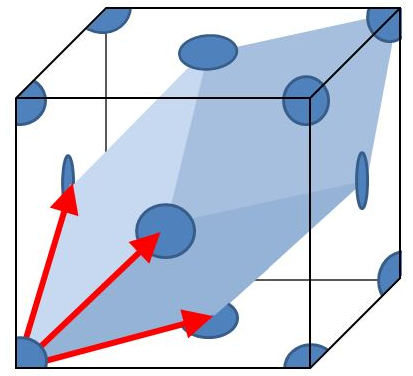
\includegraphics[height=3.5cm]{PrimitiveCellLightBlue.png}
    \caption{The Primivitive Crystal Cell is shown by the shaded parallelpiped}
    \label{fig:primitivecell}
  \end{figure}

  %\begin{figure}[h!]
    %\centering
    %% FIXME 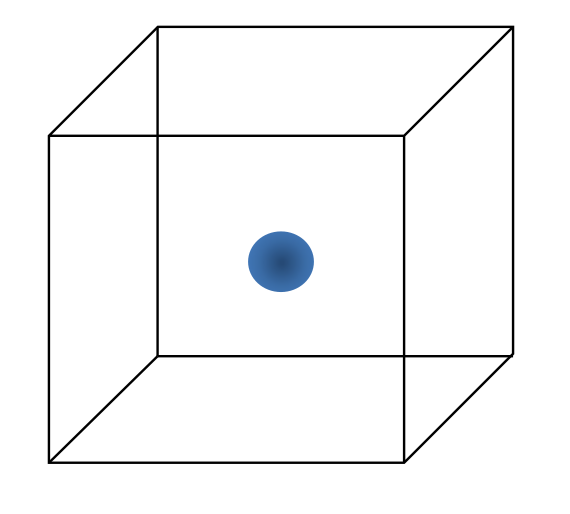
\includegraphics[height=4.5cm]{Simple_Cell.png}
    %%\caption{A Simplified Crystal Cell}
    %\label{fig:simplecell}
  %\end{figure}

%\textcolor{red}{This cell is rather complicated for the purposes of this discussion, so 
%consider instead a simplified crystal cell with one atom in its center 
%as shown in Figure \ref{fig:simplecell}. The Helmholtz free energy is 
%minimized for a fixed volume (and temperature and number of particles).  
%A fixed cubical volume called the ``bold-box" volume, $V_{bold-box}$ will 
%be used for illustration. The number density n for a collection of 
%simplified cells is simply 1 atom per fixed bold-box volume.
%\begin{displaymath}{n = \frac{N}{V}=\frac{1~\text{atom}}{V_{bold-box}}}\end{displaymath} 
%It is easier to think of 1 atom per ``box" (a reduced number density) 
%than 1 atom per some length$^3$ (the actual number density). Reduced number 
%density is given by $n^*$ and is equal to the number of atoms in a ``box" 
%of size $\sigma^3$.
%\begin{displaymath}{n^*=n\sigma^3}\end{displaymath} If $V_{bold-box}$  
%has a volume of $\sigma^3$, the reduced number density is just the number 
%of atoms in the fixed bold-box volume. 
%\begin{displaymath}\text{Reduced Number Density of the simple cell = 1 atom}\end{displaymath} 
%}
In a large collection of cells, the atom at each lattice site
will not realistically reside exactly at the lattice point. 
Statistically there will typically be a normal, or Gaussian distribution 
of positions about the lattice point as pictured in the far right box in 
Figure \ref{fig:Ensemble_Gaus}. 
A plot of a Gaussian distribution in 2-dimensions is shown in Figure~\ref{fig:Gaus_plot}
where the width of the Guassian is described by $\sigma$.  
A 3-dimensional Gaussian distribution centered at a lattice point can be used to represent 
a number density profile $n(\vec{r})$  which describes how the atoms are 
statistically distrubuted over a collection of cells. 
%In 3-dimensions, the Gaussian function takes on the form
%\begin{equation}{n(r)=\frac{1}{\left(\sqrt{2\pi}\sigma\right)^3}\int{e}^{-\frac{r^2}{2\sigma^2}}d\vec{r}}\end{equation} 
It is important to note that the number density does not change when introducing a number 
density profile. There are still the same number of atoms over some fixed volume. 
%There is still a total of one atom per ``bold box" volume.
%\begin{equation}{n=<n(\vec{r})>=\frac{1}{V_{bold-box}}\overbrace{\int_{bold-box}{n(\vec{r})}{d\vec{r}}}=\frac{N}{V}=\frac{1~\text{atom}}{V_{bold-box}}}\end{equation}
\begin{equation}{n=<n(\vec{r})>=\frac{1}{V}\int{n(\vec{r})}{d\vec{r}}=\frac{N}{V}=\frac{1~\text{atom}}{V}}\end{equation}
where $n(\vec r)$ is itself an ensemble average over all microstates, and is independent of time.
\begin{equation}n(\vec r)=~<\sum_{i=1}^N\delta(\vec r - \vec r_i)>~\end{equation}

  \begin{figure}[h!]
    \centering
    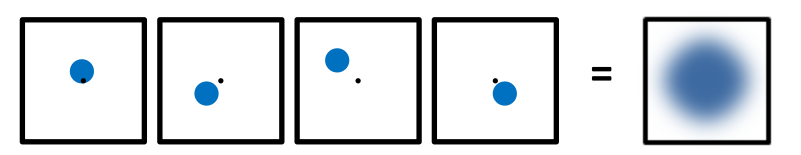
\includegraphics[height=2.5cm]{Ensemble_Gaussian.png}
    \caption{A Gaussian Distribution Number Density Profile}
    \label{fig:Ensemble_Gaus}
  \end{figure} 

 \begin{figure}[h!]
    \centering
    \includegraphics[height=6cm]{Gaussian}
    \caption{A 2D Gaussian Distribution of width 2$\sigma$}
    \label{fig:Gaus_plot}
  \end{figure}  

It may be that not all lattice sites are occupied. Vacancies can be taken 
into account while keeping %the volume of the bold box, and thus 
the overall number density the same by 
making the cells smaller. A large collection of smaller cells creates a 
new number density profile shown in Figure~\ref{fig:Ensemble_Smallcells} 
with eight smaller Gaussians each of which is now one-eigth the height. 
Instead of thinking of an atom in one of the eight small cells, the same 
Gaussian distribution can be obtained from thinking of one-eighth of an 
atom in each small cell as shown in Figure~\ref{fig:SameStatPic}. 
This makes it convenient to describe the new 
number density in terms of the fraction of vacancies, $f_v$: 
\begin{displaymath}{ n = (1-f_v){n_{no.vacancies}}}\end{displaymath} 
%\begin{align}
  %n(\vec{r})=(1-f_v)\frac{\exp^{-\frac{{\vec{r}}^2}{2{(gw)}^2}}}{\left(\sqrt{2\pi}gw\right)^3}
%\end{align}

 \begin{figure}[h!]
    \centering
    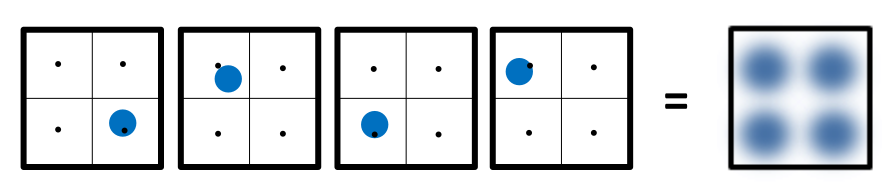
\includegraphics[height=2.5cm]{Ensemble_Smallcells.png}
    \caption{A Gaussian Distribution Number Density Profile}
    \label{fig:Ensemble_Smallcells}
  \end{figure} 

\begin{figure}[h!]
    \centering
    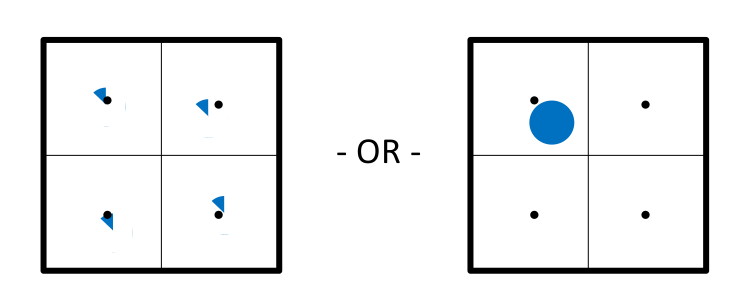
\includegraphics[height=2.5cm]{SameStatPic.png}
    \caption{Front views of a cube with eight smaller cells. The two views 
    show two ways of picturing a fraction of vacancies, $f_v$ of 7/8 which 
    give rise to the same Gaussian distribution statistically}
    \label{fig:SameStatPic}
  \end{figure} 

By varying the width of the Gaussians and the fraction of vacancies, various
number density profiles can be generated as shown in Figure~\ref{fig:Ensemble_vary}.
Once again, it is important to note that the number density is the same 
for all these number density profiles $n(\vec{r})$. 
%There is still a total of one atom per ``bold box" volume. 
%This prodcedure is used only to find the crystal free energy as the number density 
%profile for a liquid is homogeneous, as shown in Figure \ref{fig:homogen_denisty}.  
A homogeneous number density profile is used for a liquid is shown in Figure \ref{fig:homogen_denisty}.

\begin{figure}[h!]
    \centering
    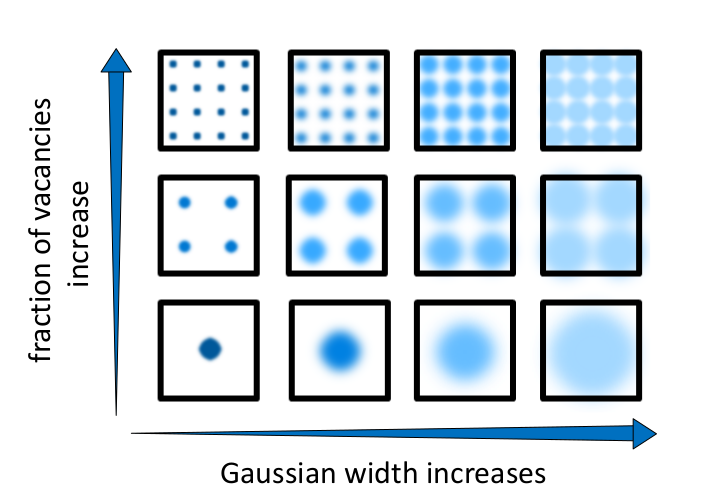
\includegraphics[height=8cm]{VaryWidthandVacancies.png}
    \caption{Several Gaussian Distribution Number Density Profiles all 
    with the same number density, that is, there is one atom over the fixed volume.}
    \label{fig:Ensemble_vary}
  \end{figure}  

 \begin{figure}[h!]
    \centering
    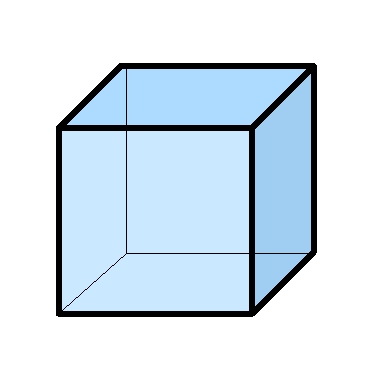
\includegraphics[height=4cm]{figs/homogeneous_bold-box.pdf}
    \caption{A homogeneouse number density profile $n(\vec{r})$}
    \label{fig:homogen_denisty}
  \end{figure}   

%Classical Density Functional Theory is used to find the equilbrium 
%Helmholtz free energy of the system at a given temperature and density
%by varying the number density profile $n(\vec{r})$ until the free energy 
%is minimized. The minimum free energy, and its corresponding number 
%density profile are then the equilibrium values for that temperature 
%and number density. 

%The number density profile is varied by varying gw and fv, and the 
For a given combination of temperature and number density, a suite of number 
density profiles are generated similiar to those represented in the example 
set of profiles shown in Figure~\ref{fig:Ensemble_vary}. 
The Helmholtz free energy $F[n(\vec{r})]$ is calculated for each number 
density profile, and also for the homogeneous number denisty profile 
characteristic of a liquid. Both the ideal and excess free energies are 
found, and added together to get the total Helmholtz free energy.
According to classical Density Functional Theory, of all the Helmholtz 
free energies calculated is the minimum Helmholtz free energy, and its 
corresponding number density profile that are the actual equilibrium values 
for that temperature and number density.
%The Helmholtz free energy is minimized for a system with a fixed temperature, 
%volume, and number of particles. Setting the number of particles to one, 
%the volume can be found from the number density.
The process is repeated to find the free energies at other combinations 
of temperatures and number densities. 

Once the Helmholtz free energy for both the crystal and liquid states of 
the fluid are found for a given temperature and density, they can be 
used to construct phase diagrams.
%compared to find the resulting state of the fluid. 
Outside the region of coexistence which exists between the liquid and 
crystal states, the fluid will be completely in a crystalline state if the 
crystal free energy is lower than the liquid free energy, and it will be 
completely in a liquid state if the liquid free energy is lower than 
the crystal free energy. Maxwell's Double Tangent Construction is used 
to determine the actual number densities of the crystal and liquid states
at the boundaries of the coexistance region for a given temperature, 
and construct phase diagrams as described in the section on The Theory of
Freezing and Maxwell's Double Tangent Construction.

\section{Our Functional for the Excess Helmholtz free energy}
In order to apply classical Density Functional Theory, the Helmholtz free 
energy must be found. Computing the ideal portion of the Helmholtz free 
energy is straightforward, but computing the excess portion of the 
Helmholtz free energy is difficult since it depends on the interatomic 
potential energy $V(r)$ between each sphere with all the other spheres, 
as is shown in Equations~\ref{eq:mayerfunction} and \ref{eq:Fexcess-simplified}.
Soft Fundamental Measure Theory is a method
developed to form an expression for the excess Helmholtz free energy without
explicitly taking into account the interaction of each sphere with all the others, 
but it must be taylored to fit a particular fluid\cite{schmidt1999density}. 
%The excess Helmholtz free energy is particular to the fluid being modeled, 
%as it depends on the interatomic potential V(r). 
It is based on the expression for the excess Helmholtz 
free energy of a homogeneous Hard-sphere fluid derived 
from Scaled Particle Theory, and given in Equation~\ref{FexfromSPT}. 
The resulting functional 
%(given in Equations~\ref{eq:F_ex-n-of-r} - \ref{eq:Phi3} and repeated here) 
is written in general form as 
\begin{align}\label{eq:Fexfunctional}
  F_{excess}[n(\vec{r})]=k_BT\int(\Phi_1(\vec{r})+\Phi_2(\vec{r})+\Phi_3(\vec{r}{)) d}\vec{r}
\end{align}
where
\begin{align}
\Phi_1 &= -n_{0}\ln(1-n_{3}) \\
\Phi_2 &= \frac{n_{1}n_{2}-\vec{n_{1}}\cdot\vec{n_{2}}}{1-n_{3}} \\
\Phi_3 &= \frac{{n_2}^3-3n_2\vec{n}_{v2}\cdot\vec{n}_{v2}+\frac{9}{2}[\vec{n}_{v2}\cdot{\overleftrightarrow{n}_{m2}}\cdot{\vec{n}_{v2}}-\operatorname{Tr}({\overleftrightarrow{n}^3_{m2}})]}{24\pi(1-n_3)^2}  
\end{align} 
and Tarazona's tensor expression~\cite{tarazonaphi3, santos2012phi3} is used 
for $\Phi_3$. The weigthed densities $n_0, n_1, n_2,$ and $n_3$ are found from
\begin{align}\label{eq:numdenprofile}
	n_i(\vec{r})=\int_{Volume}{n(\vec{r'})w_i(|\vec{r}-\vec{r'}|)d{\vec{r'}}}
\end{align}
%where the number density profile $n(\vec r)$ within the integral will be 
%given in our program by a Gaussian function centered at a lattice point, 
%and $w(r)$ is a weight function.
where the number density profile $n(\vec r)$ within the integral is given 
by a Gaussian function centered at a lattice point.
%\begin{align}
  %n(\vec r)=(1-f_v)\frac{\exp^{-\frac{r^2}{2{\sigma}^2}}}{\left(\sqrt{2\pi}\sigma\right)^3}
%\end{align}
%
There are four scaler weight functions, two vector weight functions, and 
one tensor weight function all of which 
%The weight functions $w_0(r), w_1(r), w_2(r)$ 
depend on the expression for $w_3(r)$ 
which in turn depends on the interatomic potential $V(r)$ that exists 
between the spheres, and which defines the particular fluid being modeled.
%FMT models the Hard-sphere fluid, and SFMT models fluids with soft potentials.
We introduce our temperature dependent parameters $\alpha(T)$ and $\Xi(T)$ 
to fit the functional to a WCA fluid.
The scalor weight functions are given by
\begin{align}\label{eq:weights}
  w_{0}(r) &=\frac{w_{2}}{4\pi{r}^2} \\
  w_{1}(r) &=\frac{w_{2}}{4\pi{r}} \\
  %w_{2}(r) &=-\frac{\partial{w_3(r)}}{\partial{r}}   \\
  %w_{3}(r) &=~?
  w_2(r) &=-\frac{\partial{w_3(r)}}{\partial{r}} \\
  &= \frac{\sqrt{2}}{\Xi\sqrt\pi}\exp^{-\left(\frac{r-\frac{\alpha}{2}}{\Xi/\sqrt{2}}\right)^2}  \\
  w_3(r) &=\frac{1}{2}\left[1-\operatorname{erf}\left(\frac{r-\frac{\alpha}{2}}{\frac{\Xi}{\sqrt{2}}}\right)\right]  
  %\vec{w_{1}} &= w_{1}\frac{\vec{r}}{r}   \\
  %\vec{w_{2}} &= w_{2}\frac{\vec{r}}{r}  \\
  %\overleftrightarrow{w}_{m2}(\vec{r}) &= w_2(r)\left(\frac{\vec{r}\vec{r}}{r^2}-\frac{I}{3}\right)
\end{align}
%
The vector weights are given by 
\begin{equation}\label{eq:w_v2}{  \vec{w_{2}}=w_{2}\frac{\vec{r}}{r}  }\end{equation}
\begin{equation}\label{eq:w_v1}{  \vec{w_{1}}=w_{1}\frac{\vec{r}}{r}  }\end{equation} 
The tensor weight is given by
\begin{equation}\label{eq:tensorweight-methods}\overleftrightarrow{w}_{m2}(\vec{r}) = w_2(r)\left(\frac{\vec{r}\vec{r}}{r^2}-\frac{I}{3}\right)\end{equation}
%
 \begin{figure}[h!]
    \centering
    %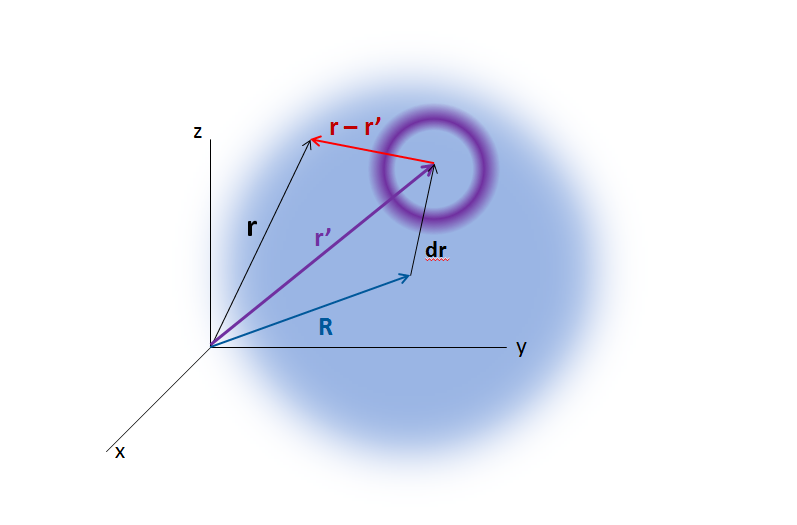
\includegraphics[height=6cm]{GaussandW2_actual.png}
    %\caption{A Gaussian centered at $\vec{R}$ is shown in blue, and a cross-sectional 
    %view of $w_2$ centered at $\vec{r}'$ is shown in purple. Here, the weight function 
    %is evaluated at $\vec{r}-\vec{r}'$ where $\vec{r}'=\vec{R}+\vec{dr}$ and $\vec{dr}$ 
    %is generated randomly according to a Gaussian distribution.} 
  \label{fig:GaussandW2_actual}
  \end{figure} 
%We use Soft Fundamental Measure Theory to form a functional for the excess 
%Helmholtz free energy appropriate for the WCA fluid by introducing our 
%
%Equation 2.94  general form of Fex for n(r)    
%\ref{eq:F_ex-n-of-r}, 
%phis 1-3   2.90, 2.91, 2.92
%\ref{eq:Phi1}, 
%\ref{eq:Phi2}, 
%\ref{eq:Phi3}, 							
%weights 2.73, 2.74, 2.89  2.79, 2.80  replace-> 2.71, 2.72		
%\ref{eq:w0}, 
%\ref{eq:w1}, 
%\ref{eq:w2}, 
%\ref{eq:w3}, 
%\ref{eq:w_v2}, 
%\ref{eq:w_v1}, 
%\ref{eq:tensorweight}, 
%%weight relations 2.75, 2.81
%\ref{w2_w3_relation}, 
%\ref{mayerder=w2convolution},

The weight functions $w_{2}(r)$ and $w_{3}(r)$ are constructed using 
Schmidt's proposed erf model~\cite{schmidt2000fluid} formed to model a steep, 
soft potential in which he set
\begin{equation}{w_3(r)=\frac{1}{2}}\left[1-\operatorname{erf}\left(\frac{r-\frac{\sigma}{2}}{\frac{\text{a}}{\sqrt{2}}}\right)\right]\end{equation} 
where $w_3(r)$ is subject to the boundary conditions $w_3(0)\approx{1}$ 
and $w_3(\infty)=0$. 
%\color{red}These boundary conditions are satisfied for $\Xi{\sqrt{2}<<\alpha}$, or $k_BT << 2.21$. \color{black} 
Our functional is  created by replacing Schmidt's parameters $\sigma$ 
and $a$ with our temperature dependent parameters $\alpha$ and $\Xi$.
\begin{equation}\sigma = \alpha(T)\text{~~~~~~~and~~~~~~~} a = \Xi(T)\end{equation}
%
The two parameters $\alpha$ and $\Xi$ are used to compensate for the 
temperature dependence that enters in through the expression for the 
error function potential $V_{erf}(r)$ which 
%is used to approximate the non-temperature dependent WCA potential that 
%is more difficult to implement computationally. The erf potential 
emerges from the relationships
that the weight functions must satisfy.
%potential at temperatures of interest will be used instead of the WCA potential. 
Using the relation
%Equation~\ref{w2_w3_relation}, shown again below, 
\begin{align}{w_{3}=\int_{r}^{\infty}{w_{2}(\vec{r})dr}\mbox{~~~~or equivilantly,~~~~}-\frac{\partial{w_3(r)}}{\partial{r}}=w_2(r)}\end{align}
and solving for $w_2(r)$
\begin{align}{\frac{dw_3(r)}{dr}\bigg|_{\infty}-\frac{dw_3(r)}{dr}\bigg|_{r}=w_2(r)}\end{align} 
we get \begin{equation}{ w_2(r)=\frac{\sqrt{2}}{\Xi\sqrt\pi}\exp^{-\left(\frac{r-\frac{\alpha}{2}}{\Xi/\sqrt{2}}\right)^2} }\end{equation} %From the deconvolution equation \begin{equation}{-\frac{1}{2}f(r)=w_0*w_3 + w_1*w_2 -\vec{w}_{V1}*\vec{w}_{V2}}\end{equation} it follows that $w_2$ must satisfy the relation
Putting $w_2(r)$ into Equation~\ref{mayerder=w2convolution}, shown again below, 
\begin{align}{\frac{df(r)}{dr}=\int_{-\infty}^{\infty}{w_2(r')w_2(r-r')dr'}}\end{align}
gives
\begin{equation}{\frac{df(r)}{dr}=\frac{1}{\Xi\sqrt{\pi}}e^{-\left(\frac{r-\alpha}{\Xi}\right)^2}}\end{equation} 
which can be integrated to obtain the Mayer function
\begin{equation}{f(r)=\int_{\infty}^r{ \frac{1}{\Xi\sqrt{\pi}}e^{-\left(\frac{r'-\alpha}{\Xi}\right)^2}{dr'}}}\end{equation} 
The Mayer function for the error function potential $V_{erf}(r)$ is thus 
given by
\begin{equation}{f(r)=-\frac{1}{2}\left[1-\operatorname{erf}\left(\frac{r-\alpha}{\Xi}\right)\right]}\end{equation} 
Combining this result with the definition of the Mayer function 
\begin{align}f(r)=e^{-\frac{V(r)}{K_BT}}-1\end{align} 
%This gives an interatomic potential of \begin{equation}{V_{erf}=-k_BT\ln(f(r)-1)}\end{equation} 
gives an expression for the for the error function potential  $V(r)=V_{erf}(r)$ 
\begin{equation}
	V_{erf}(r)=-k_BT\ln\left[\frac{1}{2}\left(\operatorname{erf}\left(\frac{r-\alpha}{\Xi}\right)+1\right)\right]
\end{equation}  

%<<<<<<< HEAD
%\davidsays{Maybe say this before presenting the weights? But also, I don't think
%there is any benefit to introducing $a$ and $\sigma$ here.} 
The weight functions $w_{2}(r)$ and $w_{3}(r)$ are constructed using 
Schmidt's proposed erf model~\cite{schmidt2000fluid} in which he set
\begin{equation}
  w_3(r)=\frac{1}{2}\left[1-\operatorname{erf}\left(\frac{r-\frac{\sigma}{2}}{\frac{\text{a}}{\sqrt{2}}}\right)\right]
\end{equation} 
where $w_3(r)$ is subject to the boundary conditions $w_3(0)\approx{1}$ 
and $w_3(\infty)=0$. 
%\color{red}These boundary conditions are satisfied for $\Xi{\sqrt{2}<<\alpha}$, or $k_BT << 2.21$. \color{black} 
Our functional is  created by replacing Schmidt's parameters $\sigma$ 
and $a$ with temperature-dependent parameters $\alpha(T)$ and $\Xi(T)$.
\begin{equation}\sigma = \alpha(T)\text{~~~~~~~and~~~~~~~} a = \Xi(T)\end{equation}

The two parameters $\alpha$ and $\Xi$ are used to compensate for the 
temperature dependence that enters in through the expression for the 
error function potential $V_{\operatorname{erf}}(r)$ which is used to approximate the
non-temperature dependent WCA potential that is more difficult to 
implement computationally. The erf potential emerges from the relationships
that the weight functions must satisfy\davidsays{In order for what?}.
%potential at temperatures of interest will be used instead of the WCA potential. 
Using Equation~\ref{w2_w3_relation}, shown again below, 
\begin{align}
  w_{3}=\int_{r}^{\infty}{w_{2}(\vec{r})dr}\mbox{~~~~or equivilantly,~~~~}-\frac{\partial{w_3(r)}}{\partial{r}}=w_2(r)
\end{align}
and solving for $w_2(r)$
\begin{align}
  \frac{dw_3(r)}{dr}\bigg|_{\infty}-\frac{dw_3(r)}{dr}\bigg|_{r}=w_2(r)
\end{align} 
we get \begin{equation}{ w_2(r)=\frac{\sqrt{2}}{\Xi\sqrt\pi}\exp^{-\left(\frac{r-\frac{\alpha}{2}}{\Xi/\sqrt{2}}\right)^2} }\end{equation} %From the deconvolution equation \begin{equation}{-\frac{1}{2}f(r)=w_0*w_3 + w_1*w_2 -\vec{w}_{V1}*\vec{w}_{V2}}\end{equation} it follows that $w_2$ must satisfy the relation
Putting $w_2(r)$ into Equation~\ref{mayerder=w2convolution}, shown again below, 
\begin{displaymath}{\frac{df(r)}{dr}=\int_{-\infty}^{\infty}{w_2(r')w_2(r-r')dr'}}\end{displaymath}
gives
\begin{equation}{\frac{df(r)}{dr}=\frac{1}{\Xi\sqrt{\pi}}e^{-\left(\frac{r-\alpha}{\Xi}\right)^2}}\end{equation} 
which can be integrated to obtain the Mayer function
\begin{equation}{f(r)=\int_{\infty}^r{ \frac{1}{\Xi\sqrt{\pi}}e^{-\left(\frac{r'-\alpha}{\Xi}\right)^2}{dr'}}}\end{equation} 
The Mayer function for the error function potential $V_{\operatorname{erf}}(r)$ is thus 
given by
\begin{equation}{f(r)=-\frac{1}{2}\left[1-\operatorname{\operatorname{erf}}\left(\frac{r-\alpha}{\Xi}\right)\right]}\end{equation} 
Combining this result with the definition of the Mayer function \begin{displaymath}f(r)=e^{-\frac{V(r)}{K_BT}}-1\end{displaymath} 
%This gives an interatomic potential of \begin{equation}{V_{\operatorname{erf}}=-k_BT\ln(f(r)-1)}\end{equation} 
gives an expression for the for the error function potential  $V(r)=V_{\operatorname{erf}}(r)$ 
\begin{equation}
	V_{\operatorname{erf}}(r)=-k_BT\ln\left[\frac{1}{2}\left(\operatorname{erf}\left(\frac{r-\alpha}{\Xi}\right)+1\right)\right]
\end{equation}  

Figure \ref{fig:weight_functions} shows a one dimensional view of the weight functions 
$w_0$, $w_1$, $w_2$, $w_3$ as they vary with distance along the z-axis. In three 
dimensions, the weighting functions $w_0$, $w_1$, $w_2$ are spherical shells 
centered at $\vec{r}$. As shown in the cross-sectional view in Figure \ref{fig:W0andW3}a, 
$w_2$ peaks at a radius of $|\vec{r}-\vec{r'}|=\frac{\alpha}{2}$, with a width determined 
by $\frac{\Xi}{\sqrt{2}}$, and edges that tapers off on either side of the peak giving 
the shell. The weighting function $w_3$, shown in Figure \ref{fig:W0andW3}b is a solid 
sphere up to $\frac{\alpha-4\Xi}{2}$ after which it tapers off. 
$\Xi$ is related to the width of the functions which 
become wider in general as the temperature increases. 
The radial distance 
to the peak is related to $\alpha$, and decreases as the temperature 
increases, that is, the shells shrink, as does 
the sphere.

\begin{figure}[h!]
    \centering
    \includegraphics[height=8cm]{weight_functions.pdf}
    \caption{The weight functions $w_0$, $w_1$, $w_2$, $w_3$ vary along the 
    z-axis for a reduced temperature of 2.}
    \label{fig:weight_functions}
  \end{figure}  

 \begin{figure}[h!]
    \centering
    \begin{subfigure}[b]{0.4\linewidth}
      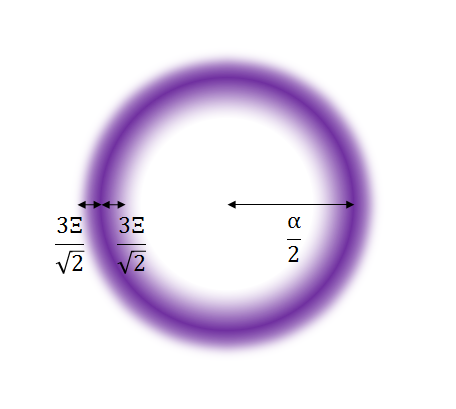
\includegraphics[height=5cm]{W2.png}
      % \includegraphics[width=5cm]{figs/w2-ring}
      \caption{A crossectional view of $w_2$}
    \end{subfigure} 
    \begin{subfigure}[b]{0.4\linewidth}
      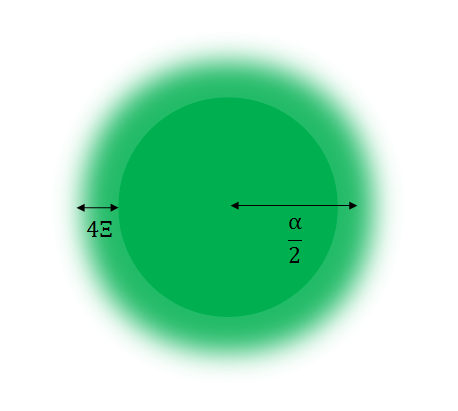
\includegraphics[height=5cm]{W3.png}
      \caption{A crossectional view of $w_3$}
    \end{subfigure} 
    \caption{Cross-sectional views of the 3D weight functions. (a) $w_2$ is a 
    spherical shell in 3D with soft edges. Weight functions $w_0$ and $w_1$ 
    have a similar shape. (b) $w_3$ is a sphere with soft edges in 3D.}
    \label{fig:W0andW3}
    \end{figure} 

Expressions for $\alpha(T)$ and $\Xi(T)$  can be found as follows. 
The parameter $\alpha(T)$ is derived by setting 
the erf potential equal to the WCA potential when $r=\alpha$, i.e. at the
maximum of $w_2(r)$,
% \begin{equation}{V_{\operatorname{erf}}(r=\alpha)=V_{WCA}(r=\alpha)}\end{equation} 
which gives us
\begin{equation}\label{alphaT}
	{\alpha(T)=\sigma\left(\frac{2}{1+\sqrt{\frac{k_BT}{\epsilon}\ln(2)}}\right)^\frac{1}{6}}
\end{equation} 
Figure \ref{fig:alphaXivsT} shows how $\alpha$ varies with temperature 
when $\sigma=1$ and $\epsilon=1$.    
\begin{figure}[h!]
    \centering
    \includegraphics[height=9cm]{plot_alpha.pdf}
    \caption{Shows the temperature dependence of $\alpha$ vs $k_BT/{\epsilon}$ 
    for $\sigma=1$ and $\epsilon=1$}
    \label{fig:alphaXivsT}
  \end{figure}

We determine value of $\Xi$ at a given temperature $T$,
by equating the second virial coefficient evaluated for the error function 
potential $V_{\operatorname{erf}}(r)$, and the second virial coefficent evaluated for the 
WCA potential $V_{WCA}$.
\begin{equation}B_{2\operatorname{erf}}(T) =B_{2WCA}(T)\end{equation}
\davidsays{I think we'd benefit from cutting much of the following, since you
show the standard equations, but skip the bit where we put in the pair potential,
which is the tricky step.}
The second virial coefficient can be derived from Euler's equation for 
the internal energy of a system, 
\begin{equation}U=TS-PV+\mu{N}\end{equation}
using the relations (discrete versions are shown here for clarity)
\begin{equation}S=-k_B\sum_{i=0}^\infty{P_i\ln{P_i}}\end{equation}
\begin{equation}U=\langle E\rangle=\sum_{i=0}^\infty{P_iE_i}\end{equation}
\begin{equation}N=\langle n\rangle=\sum_{i=0}^\infty{P_in_i}\end{equation}
which, for a canonical ensemble, gives
\begin{equation}\frac{PV}{k_BT}=N + \beta\frac{\partial{F}_{excess}}{\partial{N}}{N} - \frac{F_{excess}}{k_BT}\end{equation}
Expressing the Helmholtz free energy in terms of the pair potential 
$V(r)$ results in an equation of state expressed in terms of the virial expansion 
\begin{equation}\label{virialequation}
    \frac{PV}{k_BT}=N\left(1+\frac{N}{V}B_2(T)+\left(\frac{N}{V}\right)^2B_3(T)+ \cdot\cdot\cdot\right) 
\end{equation}
where 
\begin{equation}
	B_{2}=-\frac{1}{2}\int_{Volume}\left(e^{-\beta{V}(r)}-1\right)d\vec{r} 
\end{equation}
Evaluating $B_{2}$ for the erf potential gives
\begin{equation}
	B_{2\operatorname{erf}}(T) = \frac{\pi}{3}\Xi^3\left[\left(\frac{\alpha^3}{\Xi^3}+\frac{3\alpha}{2\Xi}\right)\left(1+\operatorname{\operatorname{erf}}\left(\frac{\alpha}{\Xi}\right)\right)+\frac{1}{\sqrt{\pi}}\left(\frac{\alpha^2}{\Xi^2}+1\right)e^{-\left(\frac{\alpha}{\Xi}\right)^2}\right]
\end{equation}
where $\alpha(T)$ is given by Equation~\ref{alphaT}. Similarly, 
$B_{2WCA}$ can be found computationally from 
\begin{equation}
	B_{2WCA}=-\frac{1}{2}\int_{Volume}\left(e^{-\beta{V}_{WCA}(r)}-1\right)d\vec{r} 
\end{equation}

\davidsays{Some of this is worth showing, but I think you're giving too many
plots here.
In general, we'd like to only show plots if we have something to say about them,
so either we want more words, or fewer figures.  e.g. what does the reader learn
from looking at your plot of $B_2$ versus $T$? If there is something they should
learn from it, then you should write that down, so they don't have to figure it
out on their own.  If there isn't anything to say, then probably you can skip
it. There \emph{are} times to just show a plot, but it's usually if it's an
prediction, and you want to say \emph{something} about the plot beyond its
existence.}
A plot of the resulting second virial coefficient $B_2(T)$  with respect 
to temperature is given in Figure~\ref{fig:B2vsT}, and a plot of $\Xi(T)$ obtained 
through this method is shown in Figure~\ref{fig:xi_fromB2vsT}. 
Figure~\ref{fig:erf_Potential_xifromB2} shows the erf potential generated with
$\alpha(T)$ and $\Xi(T)$ at a few different temperatures alongside the WCA 
potential which is not temperature dependent.

\begin{figure}[h!]
    \centering
    \includegraphics[height=8cm]{B2_vs_T_with_xi_fromB2.pdf}
    \caption{Shows the temperature dependence of $B_2$ generated from 
    matching the second virial coeficients for $V_{\operatorname{erf}}(r)$ and $V_{WCA}(r)$ 
    at each temperature.}
    \label{fig:B2vsT}
  \end{figure}

\begin{figure}[h!]
    \centering
    \includegraphics[height=8cm]{xi_fromB2.pdf}
    \caption{Shows the temperature dependence of $\Xi$ generated from 
    matching the second virial coeficients for $V_{\operatorname{erf}}(r)$ and $V_{WCA}(r)$ 
    at each temperature.}
    \label{fig:xi_fromB2vsT}
  \end{figure}

\begin{figure}[h!]
    \centering
    \includegraphics[height=8cm]{erf_Potential_xifromB2.pdf}
    \caption{Error Function Potential $V_{\operatorname{erf}}(r)$ at several temperatures 
    with $\sigma=1$, $\epsilon=1$, compared to the WCA potential $V_{WCA}(r)$ 
    shown in black.}
    \label{fig:erf_Potential_xifromB2}
  \end{figure}

%\color{red}
% FIXME \noindent!ADD PLOT of df/dr=w2*w2 !!! BUT not here!
%\color{black}

%The spheres in the WCA model fluid do not exhibit quantum interference effects as the mass of 
%the spheres, and the temperatures are taken to be large enough that the de Broglie wavelength 
%is smaller than the mean distance between the spheres. Thus, the WCA fluid can be treated as a 
%classical fluid.


%Figure \ref{fig:weight_functions} shows a one dimensional view of the weight functions 
%$w_0$, $w_1$, $w_2$, $w_3$ as they vary with distance along the z-axis. In three 
%dimensions, the weighting functions $w_0$, $w_1$, $w_2$ are spherical shells 
%centered at $\vec{r}$. As shown in the cross-sectional view in Figure \ref{fig:W0andW3}a, 
%$w_2$ peaks at a radius of $|\vec{r}-\vec{r'}|=\frac{\alpha}{2}$, a width determined 
%by $\frac{\Xi}{\sqrt{2}}$, and edges that tapers off on either side of the peak giving 
%the shell. The weighting function $w_3$, shown in Figure \ref{fig:W0andW3}b is a solid 
%sphere up to $\frac{\alpha-4\Xi}{2}$ after which it tapers off.
%The temperature dependence of parameters $\alpha$ and $\Xi$ 
%%shown in Figures~\ref{fig:alphaXivsT} and \ref{fig:xi_fromB2vsT} 
%can be related 
%to the weight functions. 
%$\Xi$ is related to the width of the functions which 
%become wider in general as the temperature increases. 
%The radial distance 
%to the peak is related to $\alpha$, and decreases as the temperature 
%increases, that is, the shells shrink, as does 
%the sphere.
%The functions can be treated as neglible outside of a distance of 
%about $3(\frac{\Xi}{\sqrt{2}}) + \frac{\alpha}{2}$ CHECK!! from the center of 
%the weight function.

 %\begin{figure}[h!]
    %\centering
    %\includegraphics[height=7cm]{weight_functions.pdf}
    %\caption{The weight functions $w_0$, $w_1$, $w_2$, $w_3$ vary along the 
    %z-axis for a reduced temperature of 2.}
    %\label{fig:weight_functions}
  %\end{figure}  

 %\begin{figure}[h!]
    %\centering
    %\begin{subfigure}[b]{0.4\linewidth}
      %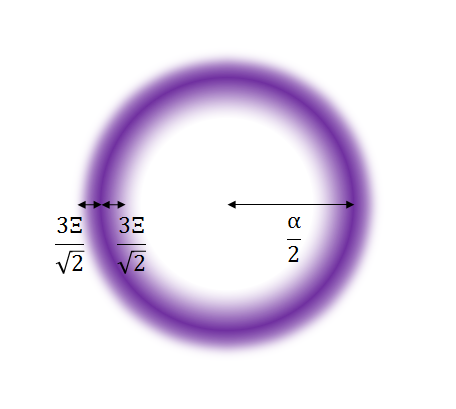
\includegraphics[height=5cm]{W2.png}
      %% \includegraphics[width=5cm]{figs/w2-ring}
      %\caption{A crossectional view of $w_2$}
    %\end{subfigure} 
    %\begin{subfigure}[b]{0.4\linewidth}
      %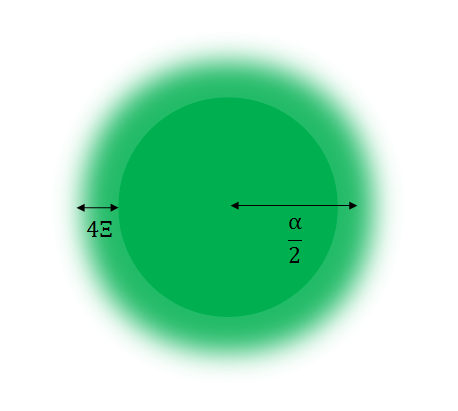
\includegraphics[height=5cm]{W3.png}
      %\caption{A crossectional view of $w_3$}
    %\end{subfigure} 
    %\caption{Cross-sectional views of the 3D weight functions. (a) $w_2$ is a 
    %spherical shell in 3D with soft edges. Weight functions $w_0$ and $w_1$ 
    %have a similar shape. (b) $w_3$ is a sphere with soft edges in 3D.}
    %\label{fig:W0andW3}
    %\end{figure} 

\section{Computing the Liquid and Crystal Helmholtz free energies}

The liquid ideal Helmholtz free energy is computed analytically 
using Equation~\ref{eq:Fideal} 
for a given homogeneous reduced density $n^*$, and reduced temperature $t^*$. 
%from the equation 
%\begin{displaymath}{\frac{F_{Hideal}}{V}=k_BTn(\ln(\frac{n*2.646476976618268x10^{-6}}{\sqrt{(k_BT)^3}})-1.0)-DELETE-EQN!}\end{displaymath} 
%\begin{align}
  %\frac{F_{Hideal}}{V}=k_BTn(\ln(n\Lambda^3)-1.0)
%\end{align}
%The quantity $\Lambda$ is the DeBroglie wavelength given by
%\begin{displaymath}{\Lambda =\sqrt{\frac{2\pi\hbar^2}{k_BTm}}}\end{displaymath}  
%where in our program we have set
%\begin{displaymath}\left(\sqrt{\frac{2\hbar^2}{m}}\right)^3=4.752731840013864\text{x}10^{-7}\color{red}units?\color{black}\end{displaymath} 
%\begin{displaymath}{m=}\end{displaymath}  
%\begin{displaymath}{\hbar=}\end{displaymath} 
%\begin{displaymath}{k_B=}\end{displaymath} 
The crystal ideal Helmholtz free energy is computed computationally 
from Equation~\ref{eq:Fideal-n(r)} with the varying number density profile given by
%\begin{align}
  %F_{ideal}[n(\vec{r})]= k_BT\int[n(\vec{r})\ln(n(\vec{r})\Lambda^3)-n(\vec{r})]dV
%\end{align} 
\begin{align}
  n(|\vec{r}-\vec{R_j}|)=\sum_j{(1-f_v)\frac{e^{-\frac{{|\vec{r}-\vec{R_j}|}^2}{2{\sigma}^2}}}{\left(\sqrt{2\pi}\sigma\right)^3}}
\end{align}
where $\vec R_j$ is the position vector of the jth lattice site.
%For small gw values it is assumed that the Guassians do not overlap, 
%in which case the equation for the free energy can be simplified, and solved
%analytically with the result
%\begin{equation}
 %F_{Cideal}=(1-f_v)k_BT\left(\ln((1-f_v)\Lambda^3)-3\ln(\sqrt{2\pi{gw}})-\frac{5.0}{2}\right)
%\end{equation}
%For larger gw values it is assumed that the Gaussians do overlap, 
%and so the free energy is caluculated computationally. First dx is scaled by gw,
%\begin{equation}
  %dx_{scaled} = (dx_{input})(gw)
%\end{equation}
%and then $n(\vec{r})$ is computed at one position of $\vec{r}$ within the 
%primitive cell taking into account the contribution of Gaussians from 
%many (5x5x5) nearby cells whose centers are given by $R_i$.
%%\begin{displaymath}{n(|\vec{r}-\vec{R_i}|)+=\frac{(1-f_v)\exp^{-\frac{{|\vec{r}-\vec{R_i}|}^2}{2{(gw)}^2}}}{\left(\sqrt{2\pi}gw\right)^3}}\end{displaymath}
%The contribution to the free energy of $n(\vec{r})$ at the one position is then
%added to the accumulating sum.
%%\begin{displaymath}{cF_{ideal}+=k_BTn(ln(\frac{(n)2.646476976618268x10^{-6}}{\sqrt{(k_BT)^3}})-1.0)dV-DELETE-EQN!}\end{displaymath}
%%\begin{displaymath}{cF_{ideal}+=k_BTn(\ln(n\Lambda^3)-1.0)dV}\end{displaymath}
%This process is repeated for all positions within one primitive cell to get the
%crystal ideal free energy for the primitive cell. This energy is then divided by
%the volume of the primitive cell to get the crystal ideal free energy per
%volume.
%
The liquid excess Helmholtz free energy is computed analytically  
%for a given homogeneous reduced density $n^*$, and reduced temperature $t^*$ 
using SFMT Equations~\ref{eq:Fexfunctional} through \ref{eq:tensorweight-methods} 
with a uniform number density profile, n that does not depend on $\vec r$. 
%done in hf.energy() note- does not depend on fv or gw but does use SFMT):
%\begin{displaymath}{\frac{F_{Hexcess}}{V} = k_BT(\Phi_1+\Phi_2+\Phi_3)}\end{displaymath} 
%For the case of a homogeneous number density n, $\Phi_2$, and $\Phi_3$ simplify to:
%\begin{displaymath}{\Phi_1= -n_0\ln(1-n_3)}\end{displaymath} 
%\begin{displaymath}{\Phi_2= \frac{n_1n_2}{1-n_3}}\end{displaymath} 
%\color{red}\begin{displaymath}{\Phi_3=\frac{n_2^3}{24\pi(1-n_3)^2}}\end{displaymath}\color{black}
%The weighted densities are found from
%\begin{displaymath}{n_i=nw_i}\end{displaymath} 
%where the weights $w_i$ are given by Equations~\ref{eq:weights}.

The crystal excess Helmholtz free energy is computed  
using SFMT with a number density profile 
%$n(|\vec r'-\vec R_j|)$ 
%used in Equation~\ref{eq:numdenprofile} 
%that is composed of Guassian distributions centered at each lattice site.
that consists of Guassian distributions 
%$n(|\vec r'-\vec R_j|)$ 
centered at lattice sites specified by position vectors $\vec R$. 
%where j indicates the jth lattice site.
%specified by position vectors $\vec R$.
The weight functions $w_i(|\vec r - \vec r'|)$ are centered at $\vec r'$,
as shown for $w_2$ in Figure~\ref{fig:GaussandW2_actual}. 
But because the weight function is a function of the magnitude of the 
difference between $\vec r$ and $\vec r'$, it can be thought of as 
centered at $\vec r$, as shown in Figure~\ref{fig:GaussandW2_thinkas}. 
Keeping the weight function centered at $\vec r$, 
%, and setting $\vec{dr}=\vec r' - \vec{R}_j$, 
% and 
%a vector $\vec dr$ is defined to be the difference between $\vec R$ and $\vec r'$.
% $\vec dr = \vec r' - \vec R$.
%First dx is scaled by $\Xi$ or gw, whichever is larger \begin{displaymath}{dx_{scaled}=(dx_{input})(\Xi + gw)}\end{displaymath}
%Then the crystal, or inhomogeneous, excess free energy is found from
%\begin{displaymath}{F_{Cexcess}[n(\vec{r})]= k_BT\int(\Phi_1(\vec{r})+\Phi_2(\vec{r})+\Phi_3(\vec{r}{)) d}\vec{r}}\end{displaymath} 
Monte-Carlo integration can be used to compute the weighted densities $n_i(\vec r)$
%$n_0(\vec{r})$, $n_1(\vec{r})$, $n_2(\vec{r})$, $n_3(\vec{r})$
%form $\Phi_1(\vec{r})$, $\Phi_2(\vec{r})$, and $\Phi_3(\vec{r})$.
%
\begin{figure}[h!]
   \centering
   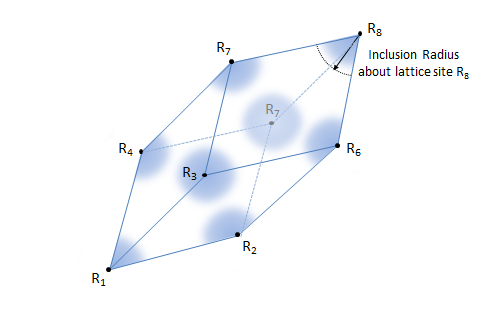
\includegraphics[height=5cm]{InclusionRadius.png}
   \caption{The Gaussians at each lattice point are of width gw. 
   After a radius of few gw's the Gaussians go to zero and can be neglected.}
   \label{fig:InclusionRadius}
\end{figure} 
%
%\textcolor{red}{The center of the weighting function is placed at some vector $\vec{r}=\vec{r}_k$ 
%within the primitive cell, and a vector $\vec{R}_j$ to the center of one of 
%the Gaussians
%is selected
%that is within the primitive cell, or one of the 
%neighboring cells within an inclusion radius as Gaussians 
%farther away will not contriubute much (see Figure \ref{fig:InclusionRadius}).}
%
%The weighted densities $n_0(\vec{r}_k)$, $n_1(\vec{r}_k)$, $n_2(\vec{r}_k)$, 
%$n_3(\vec{r}_k)$ at $\vec{r}_k$ are then computed using the weight functions 
%$w_0(|\vec{r}_k-\vec{R_j}-\vec{dr}|)$, $w_1(|\vec{r}_k-\vec{R_j}-\vec{dr}|)$, 
%$w_2(|\vec{r}_k-\vec{R_j}-\vec{dr}|)$, $w_3(|\vec{r}_k-\vec{R_j}-\vec{dr}|)$ 
%where $\vec{dr}$ is a vector from the Gaussian centered at $\vec{R}_j$ to 
%some point in space.
%Monte-Carlo integration works 
by randomly generating vectors
$\vec r' -\vec R$ according to a Gaussian distribution. 
%Setting $\vec{r}'=\vec{R}_j + \vec{dr}$, and 
%Setting $\vec{dr}=\vec r' - \vec{R}_j$,  and 
%$n(\vec{r'})=(1-f_v)n_g(\vec{r'})$ where $n_g(\vec{r'})$ 
%where $n_g(\vec{r'})$ is the gaussian number density profile for no vacancies. 
Only lengths for $\vec r'- \vec R$ that are within an inclusion radius
about a lattice site, like that shown in Figure \ref{fig:InclusionRadius}, 
will be taken into account as Gaussians 
farther away will not contriubute much.
The equation for the contribution to the weighted density from a 
Gaussian centered at the jth lattice site located at $\vec R_j$ is given by
%lattice point located at $\vec R_j$ is given by
\begin{equation}{n_i(\vec r)= \int_{r'}{(1-f_v)n(\vec r' - \vec R_j)w_i(|\vec{r}-\vec{r}'|)} {d}\vec{r}'}\end{equation} 
and is implemented computationally in the form
\begin{equation}{n_i(\vec r)= \sum_{r'}{(1-f_v)n(\vec r' -\vec R_j)w_i(|\vec{r}-\vec{r}'|)dV}}\end{equation} 
which can be written as
\begin{equation}{n_i(\vec r)= \sum_{NumPoints}(1-f_v)P_{r'}w_i(|\vec{r}-\vec{r}'|)}\end{equation} 
NumPoints is the number of vectors $\vec r' - \vec R_j$ randomly generated about the jth lattice site, 
%and $n_g(\vec{r'} - \vec R_j)$ 
%(the value of the Gaussian at a radius of $|\vec{r'}|$) 
%(the value of the Gaussian at a radius of $|\vec{dr}|$) 
and $n(\vec r' - \vec R_j)$
is equal to a probability density 
which when multiplied by dV gives the probability $P_{r'}$ at which the value of 
$w_i(|\vec{r}-\vec{r}'|)$ will occur. 
Using the relation
\begin{displaymath}{f_{average}=\sum_i^N{P_if_i}=\sum_i{\frac{f_i}{N}}}\end{displaymath} 
$n_i(\vec{r})$ can be expressed as the average value of $(1-f_v)w_i(|\vec{r}-\vec{r}'|)$:
\begin{equation}{n_i(\vec{r})=\sum_{\text{NumPoints}}\frac{(1-f_v)w_i(|\vec{r}-\vec{r}'|)}{\text{NumPoints}}}\end{equation}
This process is repeated to get the contributions to the weighted density 
$n_i(\vec r)$ from the Guassians around each lattice point which begin to 
merge together as the width of the Guassians increases.
All the contributions are then added together 
to get the final value of the weighted density at some point $\vec r$.

The result can be made more accurate by increasing NumPoints (the 
number of vectors randomly generated), and by using antithetic variates.
%
 \begin{figure}[h!]
    \centering
    %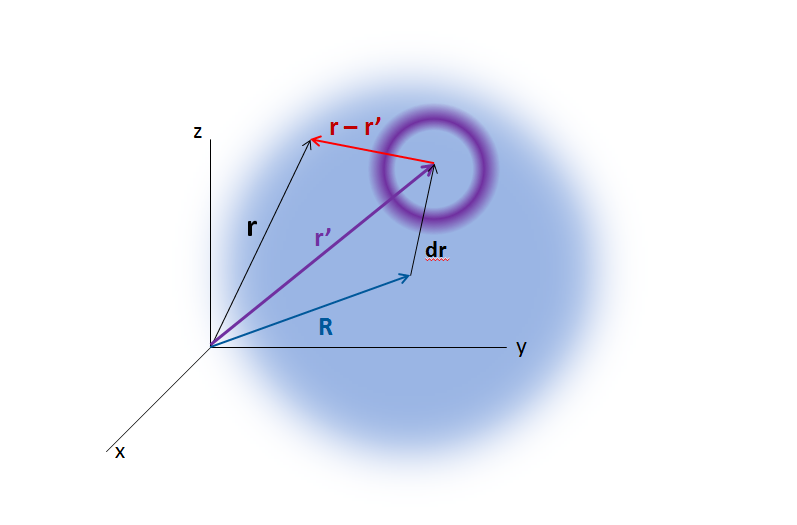
\includegraphics[height=6cm]{GaussandW2_actual.png}
    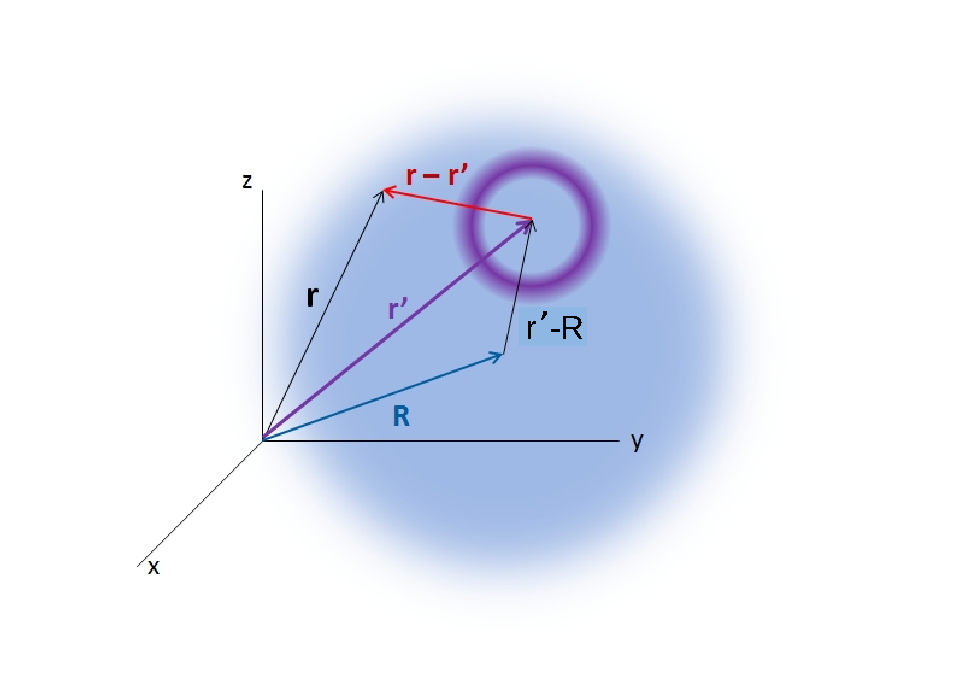
\includegraphics[height=7cm]{figs/weightandGauss1.pdf}
    %\caption{A Gaussian centered at $\vec{R}$ is shown in blue, and a cross-sectional 
    %view of $w_2$ centered at $\vec{r}'$ is shown in purple.} 
    \caption{A Gaussian distribution about a lattice site located at 
    $\vec R$ is shown in blue, and a cross-sectional 
    view of $w_2$ centered at $\vec{r}'$ is shown in purple.} 
    %Here, the weight function 
    %is evaluated at $\vec{r}-\vec{r}'$ where $\vec{r}'=\vec{R}+\vec{dr}$ and $\vec{dr}$ 
    %is generated randomly according to a Gaussian distribution.} 
  \label{fig:GaussandW2_actual}
  \end{figure} 
%
 \begin{figure}[h!]
    \centering
    %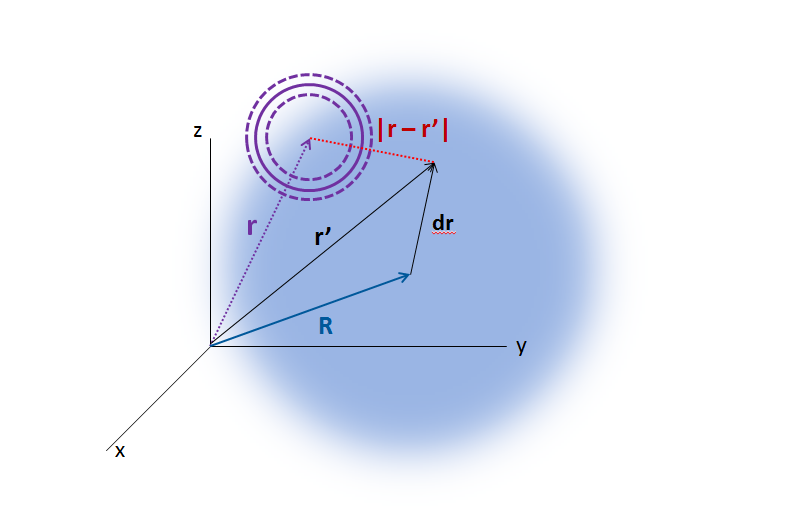
\includegraphics[height=6cm]{GaussandW2_thinkas.png}
    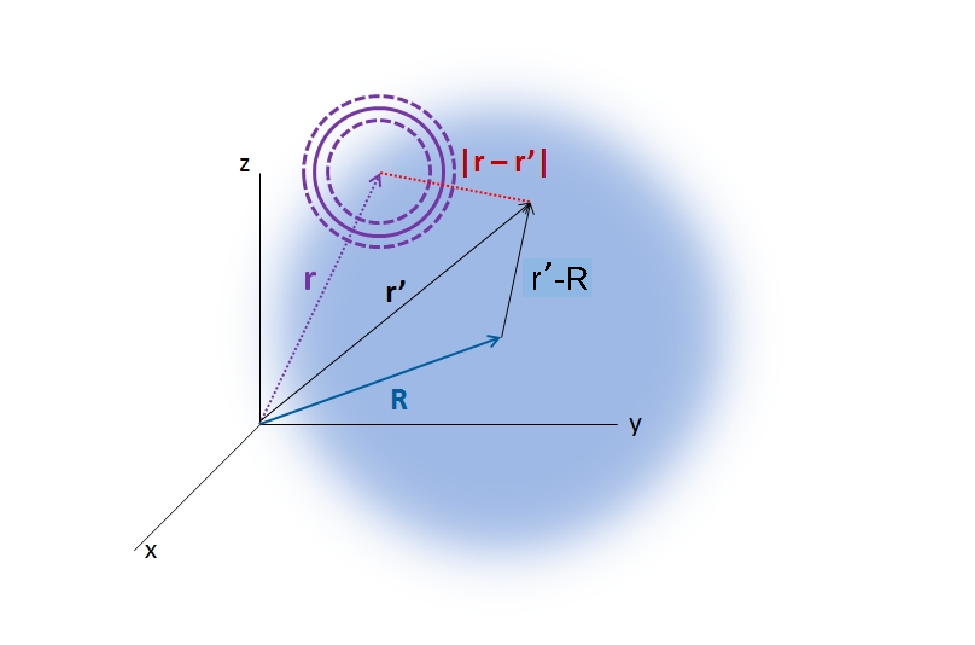
\includegraphics[height=7cm]{figs/weightandGauss2.pdf}
    \caption{An alternative way of viewing Figure~\ref{fig:GaussandW2_actual} where 
    the weight function, shown by the purple dashed lines, is centered at $\vec{r}$,  
    and fixed in place as $\vec r' - \vec R$
    %as $\vec{dr}=\vec{r}'-\vec{R}$ 
    varies randomly with a probability according to a Gaussian distribution.} 
  \label{fig:GaussandW2_thinkas}
  \end{figure} 
%
%Monte-Carlo integration is employed to more efficiently 
%compute the weighted densities used to calculate the excess free energy which is then 
%added to the ideal free energy (computed analytically) to get the total free energy 
%which is minimized. 
%
%-------Antithetic-------------------
%To further reduce the error in the average, antithetic variates are used. 
%Rather than computing an average of a set of random points, 
%antithetic variates can be used to reduce error. 
To use antithetic variates,
each randomly generated  vector is paired with a 
vector of equal magnitude, but opposite in direction. 
%as shown in Figure \ref{fig:AntitheticVariate}. 
%The quantity that is a function of the randomly generated vector
%now has two values that can be averaged to get a more accurate value. 
First order error is reduced
%in the quantity that is a function of the randomly generated vector
%average by filtering out an erroneous offset of values 
%along the line connecting the two points 
by averaging the two results that depend on the vectors, one of 
which may be erroneously higher than it should be while the other is 
erronesously lower than it should be.

 \begin{figure}[h!]
    \centering
    %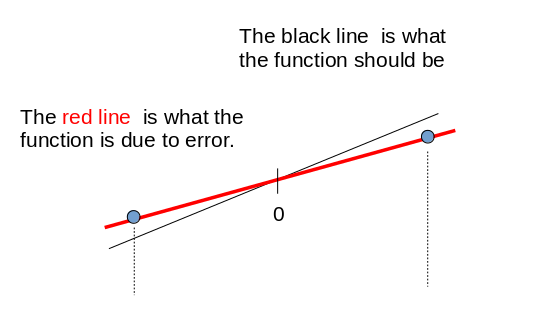
\includegraphics[height=4cm]{AntitheticVariate.png}
    %\caption{Antithetic variates reduce first order error in an average. 
    %Each point in the average is paired with another point from along 
    %the same line as the first, and at an equal, but opposite distance.}
    \label{fig:AntitheticVariate}
  \end{figure} 
%Incorporating antithetic variates $-\vec{dr}$ for every $\vec{dr}$ equation ?? becomes:
%\begin{displaymath}{n_i(\vec{r}_k, \vec{R}_j)=\sum_{NumPoints}\frac{1}{2}\frac{(1-f_v)\left[w_i(|\vec{r}-\vec{R_j}-\vec{dr}|) +w_i(|\vec{r}-\vec{R_j}+\vec{dr}|)\right]}{NumPoints}}\end{displaymath}   
%The process is repeated for all the other $\vec{R}_j$'s to get the total 
%weighted densities at vector $\vec{r}_k$ due to all the Gaussians. 
%\begin{displaymath}{n_i(\vec{r}_k)=\sum_j{n_i(\vec{r}_k, \vec{R}_j)}}\end{displaymath}
%Then the entire process repeated for each vector $\vec{r}_k$ to get the 
%total weighted densities $n_i(\vec{r})$ as a function of the position $\vec{r}$. 

The standard error of the mean (SEM) is given in general by
\begin{equation}{SD_{mean}=\frac{SD}{\sqrt{N}}}\end{equation} 
%which gives a measure of the error in $n_3=\overline{w}_3$:
To compute the error, the standard deviation of weight function $w_3$ is used 
\begin{equation}SD=\sqrt{\overline{w_3^2}-(\overline{w}_3)^2}\end{equation} 
\begin{equation}{Error=\sqrt{\frac{\overline{w_3^2}-(\overline{w}_3)^2}{\text{NumPoints}}}}\end{equation} 
NumPoints, the number of vectors randomly generated, is increased until
\begin{equation}{Error<\frac{|1-n_3|}{4}}\end{equation}
where the maximum value that the weighted density $n_3$ 
%(which equals $\overline{w}_3$) 
can properly have is 1.

%Figure \ref{fig:GaussandW2_actual} ......

\chapter{Results and Discussion}

Phase diagrams for the WCA fluid are shown in Figures~\ref{fig:Phase_Diagram_of_T_vs_n} 
and \ref{fig:Phase_Diagram_P_vs_T}. In all cases $\sigma=1$ and $\epsilon=1$. 
In Figure~\ref{fig:Phase_Diagram_of_T_vs_n} the reduced temperature $T^*=\frac{kT}{\epsilon}$ 
is plotted against the reduced number density $n^*=n\sigma^3$ for temperatures of kT = 0.5 to 3.0. 
The red area is fluid, and the blue area is crystal. The gray area that separates the fluid, 
and the crystal regions is where some fluid and crystal exist together at varying porportions. 
The region of coexistence slants slightly to the right toward higher density as the temperature 
increases. This is expected since at higher temperatures, the fluid would have to be under 
greater compression before forming a solid. The white lines show results from Monte-Carlo 
simulations of the WCA fluid~\cite{May}. Overall, the general shape, and position of the lines correspond
fairly closely to the edges of the region of coexistance predicted from the DFT method, 
but the width of the coexistance region is about one-third larger for the Monte-Carlo results 
for most temperatures. The white line on the right, representing the density of the solid at 
each temperature, is in fairly good aggreement with our DFT results for all temperatures. 
However, the white line on the left, representing the density of the liquid at each temperature, 
is consistenty farther left than the liquid transition densities our method predicted.

%Figure~\ref{fig:Phase_Diagram_of_T_vs_n_AS} shows our results for a wider 
%range of reduced temperatures from kT=0.5 to 38. The white lines show the results
%of molecular simulations of the WCA fluid made by Ahmed and Sadus~\cite{ahmedsadus}.
%As can be seen in the figure, the region of coexistence in our simulations 
%falls within the region of coexistance predicted by Ahmed and Sadus at almost 
%all temperatures from approximately kT=0.5 to 28. At the low temperature of kT=0.5,
%the width of the coexistance regions are nearly the same, while moving to 
%higher temperatures,the width of our coexistance region ranges from about 
%one-half to one-forth the size. Although, our coexistence region is only 
%about one-forth the size at kT=28, it is centered within the coexistence 
%region predicted by Ahmed and Sadus. 

\begin{figure}
  \centering
  %\includegraphics[width=\columnwidth]{figs/Phase_Diagram_of_T_vs_n}
  \includegraphics[height=10cm]{figs/Phase_Diagram_of_T_vs_n}
  \caption{Phase Diagram of the reduced temperature verses the reduced density for the WCA fuild. 
  White lines show the liquid and solid transition densities at each temperature from 
  Monte-Carlo simulations of the WCA fluid. The gray region is the region of coexistence.}
  \label{fig:Phase_Diagram_of_T_vs_n}
\end{figure}

\begin{figure}
  \centering
  %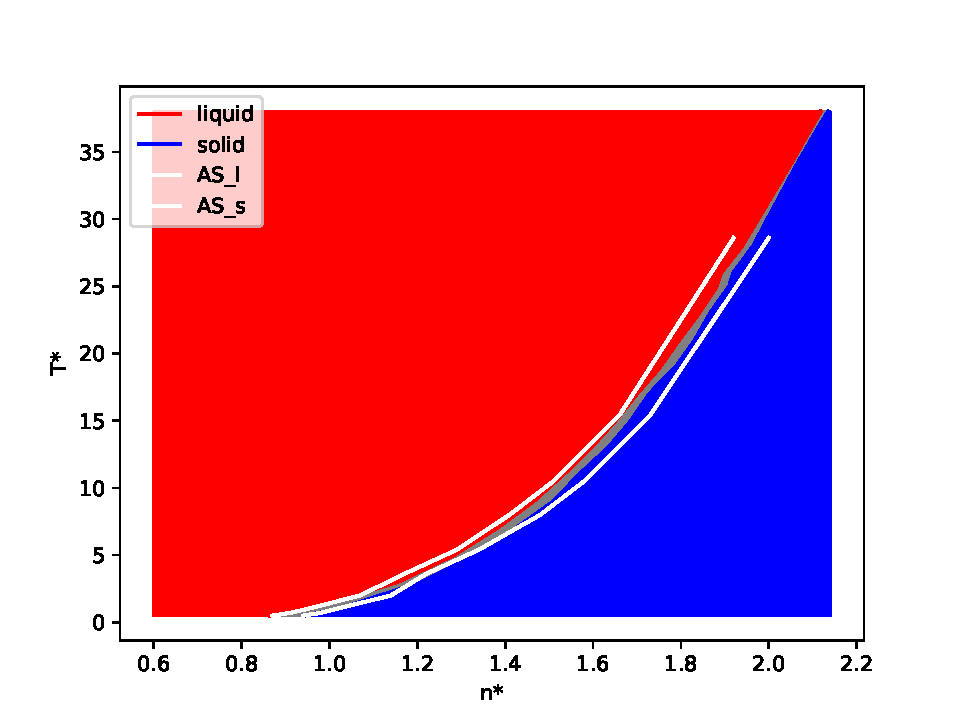
\includegraphics[width=\columnwidth]{figs/Phase_Diagram_of_T_vs_n_AS}
  %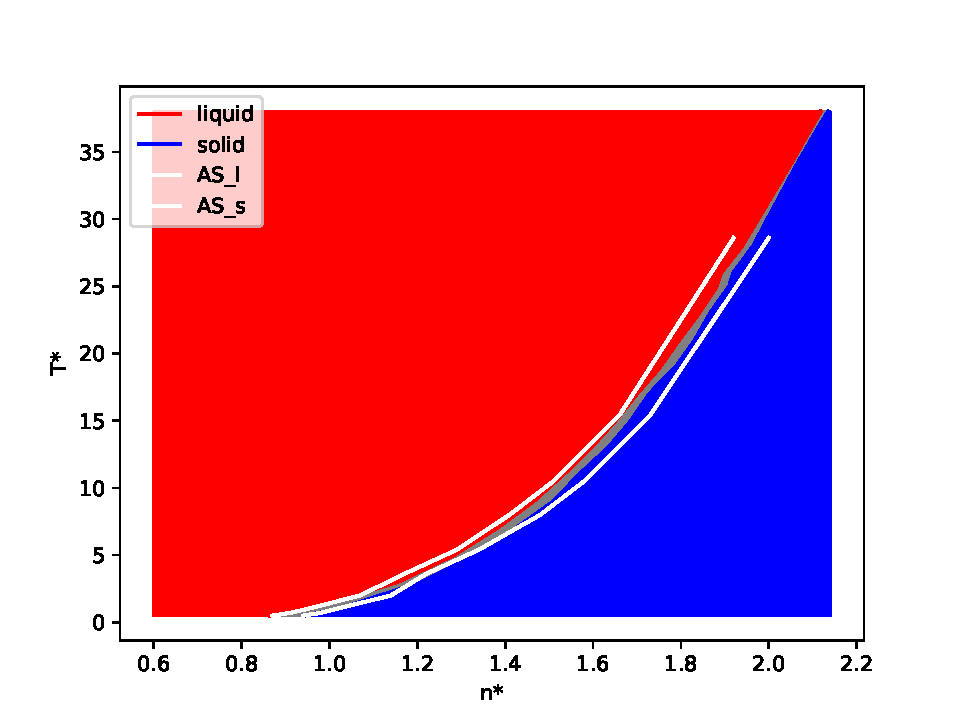
\includegraphics[height=10cm]{figs/Phase_Diagram_of_T_vs_n_AS}
  %\caption{Phase Diagram of the reduced temperature verses the reduced density for the WCA fuild. 
  %White lines show the liquid and solid transition densities at each temperature from 
  %simulations of a WCA fluid by Ahmed and Sadus~\cite{ahmedsadus}. The gray region is the region of coexistence.}
  \label{fig:Phase_Diagram_of_T_vs_n_AS}
\end{figure}

Figure~\ref{fig:Phase_Diagram_P_vs_T} shows the reduced pressure $p^*=\frac{P\sigma^3}{\epsilon}$ 
plotted against the reduced temperature for temperatures of kT = 0.5 to 3.0. Again, the red area 
is fluid, and the blue area is crystal. The general trend of the values for the transition 
temperatures and pressures is what would be expected, with the WCA fluid becoming a solid at
a higher pressure for a higher temperatuer, or becoming a liquid at a higher temperature 
for a higher pressure. But the transition pressures and temperatures are consistently higher 
than the Monte-Carlo simulations shown by the white line, and the descripancy grows as 
the temperature increases. 
%Figure~\ref{fig:Phase_Diagram_P_vs_T_AS} shows our results for a larger 
%range of reduced temperatures from kT=0.5 to 38, compated with the results
%from Ahmed and Sadus's molecular simulations. Here again, our transition 
%pressures and temperatures are consistently higher.

\begin{figure}
  \centering
  %\includegraphics[width=\columnwidth]{figs/Phase_Diagram_of_P_vs_T}
  \includegraphics[height=10cm]{figs/Phase_Diagram_of_P_vs_T}
  \caption{Phase Diagram of the reduced pressure verses the reduced temperature. 
  The white line marks the boundary from Monte-Carlo simulations.}
  \label{fig:Phase_Diagram_P_vs_T}
\end{figure}

\begin{figure}
  \centering
  %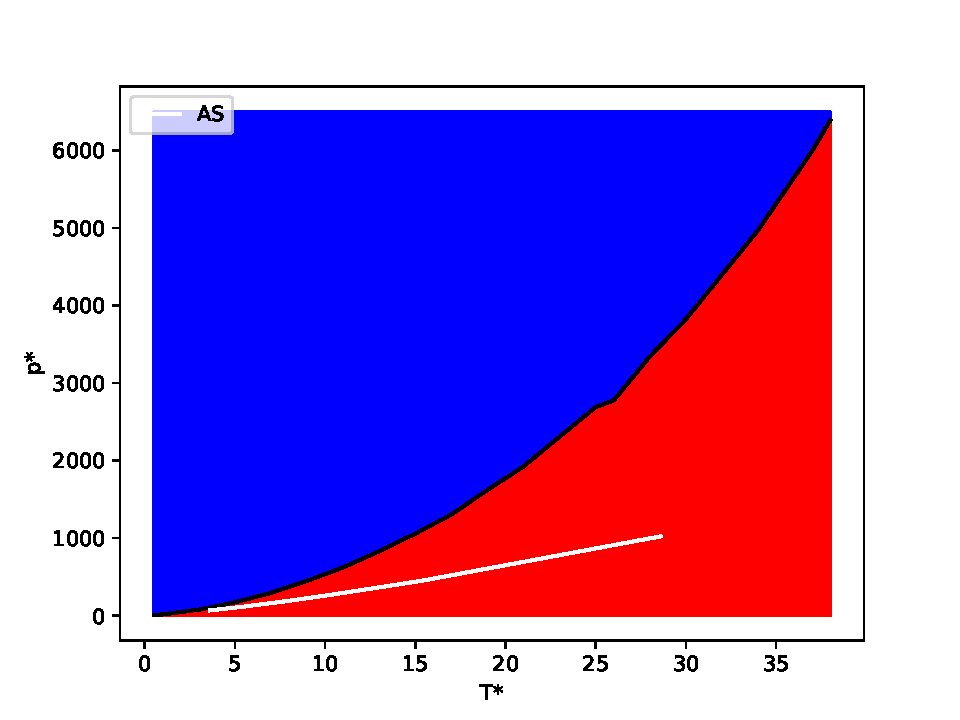
\includegraphics[width=\columnwidth]{figs/Phase_Diagram_of_P_vs_T_AS}
  %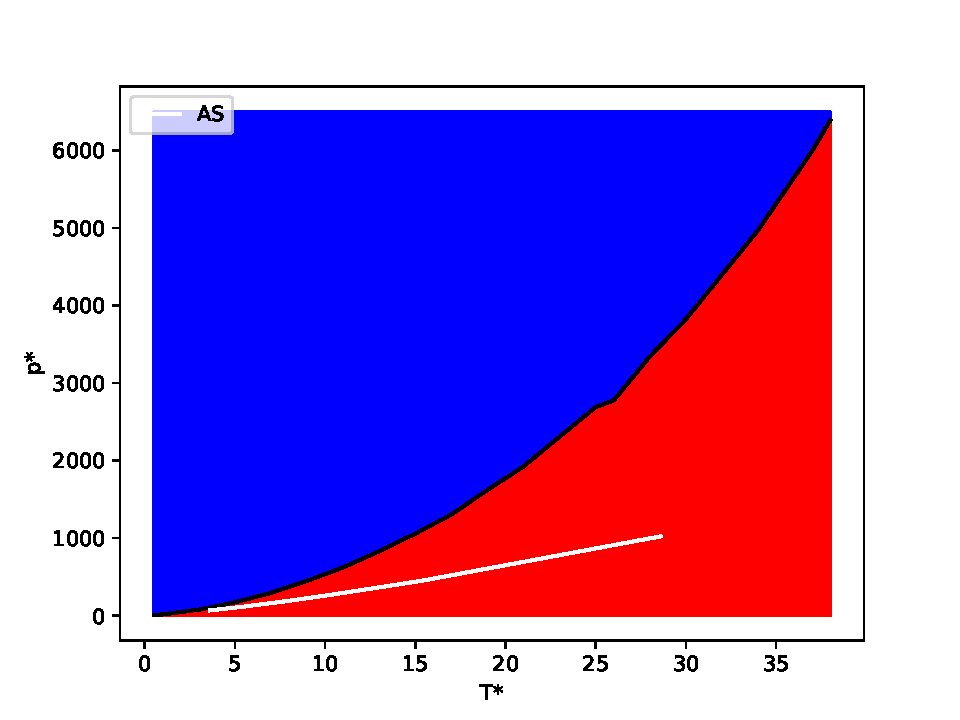
\includegraphics[height=10cm]{figs/Phase_Diagram_of_P_vs_T_AS}
  %\caption{Phase Diagram of the reduced pressure verses the reduced temperature. 
  %The white line marks the boundary from simulations by Ahmed and Sadus~\cite{ahmedsadus}.}
  \label{fig:Phase_Diagram_P_vs_T_AS}
\end{figure}

%Figure~\ref{fig:p-vs-T_at_fixed_density} shows individual plots of the 
%reduced pressure versus the reduced temperature at fixed reduced densities 
%from $n^*$ = 0.7 to 1.2. As can be seen by comparison with Figure 
%\ref{fig:Phase_Diagram_P_vs_T_AS}, the plotted lines display kinks when 
%the WCA fluid transistions into a solid. These downward bends align to 
%form the curved interface separating the blue and red areas in 
%Figures~\ref{fig:Phase_Diagram_P_vs_T} and \ref{fig:Phase_Diagram_P_vs_T_AS}.

\begin{figure}
  \centering
  %\includegraphics[width=\columnwidth]{figs/p-vs-T_at_fixed_n_noMC}
  %\caption{Plot of the reduced pressure verses the reduced temperature. 
  %The lines bending downward indicate freezing.}
  \label{fig:p-vs-T_at_fixed_density}
\end{figure}

%More plots...

%\begin{figure}
  %\centering
  %\includegraphics[width=\columnwidth]{figs/T-vs-n_at_fixed_P_moreTemp}
  %\caption{Plot of the reduced temperature verses the reduced density. 
  %The grey region indicates coexistence.}
  %\label{fig:T-vs-n_at_fixed_P}
%\end{figure}

%\begin{figure}
  %\centering
  %%\includegraphics[width=\columnwidth]{figs/p-vs-V_at_fixed_T}
  %\caption{Plot of the reduced pressure verses the reduced volume. 
  %The grey region indicates coexistence.}
  %\label{fig:p-vs-V_at_fixed_T}
%\end{figure}

%\begin{figure}
  %\centering
  %%\includegraphics[width=\columnwidth]{figs/p-vs-n_at_fixed_T}
  %\caption{Plot of the reduced pressure verses the reduced density. 
  %The grey region indicates coexistence.}
  %\label{fig:p-vs-n_at_fixed_T}
%\end{figure}

\chapter{Conclusion}
In this paper we were sucessful in predicting the freezing of a 
Weeks-Chandler-Anderson fluid using our SFMT functional built by 
forming temperature dependent parameters $\alpha(T)$ and $\Xi(T)$ to use 
in Schmidt's erf model to better fit our results to those expected for a
WCA fluid. We were able to generate a temperature-density 
phase diagram that yielded coexistence regions that approximately 
matched the Monte-Carlo
% and molecular simulation 
results. 
%for values of kT=0.5 to 3. 
%kT=0.5 to 38
We are also able to generate a pressure-temperature
phase diagram with a shape that is expected, but the transition 
temperatures and pressures were too high. 



\backmatter

\chapter{Appendix}

\section{Fourier Transform of Weight Function $w_0(r)$}
\begin{equation}{w_0(r)=\frac{w_2(r)}{4{\pi}r^2}}\end{equation}
where
\begin{equation}{w_2(r)=\frac{\sqrt{2}}{\Xi\sqrt{\pi}}e^{-\left(\frac{r-\frac{\alpha}{2}}{\frac{\Xi}{\sqrt{2}}}\right)^2}}\end{equation}
temporarily set 
\begin{equation}{a=\frac{\Xi}{\sqrt{2}}}\end{equation}
\begin{equation}{w_0(r)=\frac{1}{4{\pi}\sqrt{\pi}a}\left(\frac{1}{r^2}\right)e^{-\left(\frac{r-\frac{\alpha}{2}}{a}\right)^2}}\end{equation}

\begin{equation}{\widetilde{w}_0(\vec{k})=\int_{0}^{\infty}\int_{-1}^{1}\int_{0}^{2\pi}w_0(r)e^{-i\vec{k}\cdot{\vec{r}}}r^2d{r}d{\cos\theta}d{\phi}}\end{equation}
Set $\vec{k}$ in the direction of $\hat{z}$ 
\begin{equation}{\widetilde{w}_0(k)=\int_{0}^{\infty}\int_{-1}^{1}\int_{0}^{2\pi}w_0(r)e^{-ikr\cos\theta}r^2d{r}d{\cos\theta}d{\phi}}\end{equation}

Calculate $\widetilde{w}_0(k)$ 
\begin{equation}{\widetilde{w}_0(k)=\frac{1}{4{\pi}\sqrt{\pi}a}\int_{0}^{\infty}\left(\frac{1}{r^2}\right)e^{-\left(\frac{r-\frac{\alpha}{2}}{a}\right)^2}r^2\left[\int_{-1}^{1}e^{-ikr\cos\theta}d{\cos\theta}\left(\int_{0}^{2\pi}d{\phi}\right)\right]d{r}}\end{equation}

\begin{equation}{\widetilde{w}_0(k)=\frac{2\pi}{4{\pi}\sqrt{\pi}a}\int_{0}^{\infty}e^{-\left(\frac{r-\frac{\alpha}{2}}{a}\right)^2}\left(\int_{-1}^{1}e^{-ikr\cos\theta}d{\cos\theta}\right)d{r}}\end{equation}

Set the lower limit to $-\infty$  since the integrand is nearly zero by the time r is zero. 
\begin{equation}{\widetilde{w}_0(k)=\frac{1}{\sqrt{\pi}ka}\int_{-\infty}^{\infty}e^{-\left(\frac{r-\frac{\alpha}{2}}{a}\right)^2}\frac{\sin(kr)}{r}d{r}}\end{equation}

\begin{equation}{\widetilde{w}_0(k)=\frac{\sqrt{\pi}}{2ka}e^{-\left(\frac{\alpha}{2a}\right)^2}\left[\operatorname{erf}\left(\frac{ka}{2}+i\frac{\alpha}{2a}\right)+\operatorname{erf}\left(\frac{ka}{2}-i\frac{\alpha}{2a}\right)\right]}\end{equation}
 
Putting in $a=\frac{\Xi}{\sqrt{2}}$ the final equation for $\widetilde{w}_0(k)$ becomes
\begin{equation}{\widetilde{w}_0(k)=\frac{\sqrt{\pi}}{\sqrt{2}k\Xi}e^{-\left(\frac{\alpha^2}{2\Xi^2}\right)}\left[\operatorname{erf}\left(\frac{k\Xi}{2\sqrt{2}}+i\frac{\alpha}{\sqrt{2}\Xi}\right)+\operatorname{erf}\left(\frac{k\Xi}{2\sqrt{2}}-i\frac{\alpha}{\sqrt{2}\Xi}\right)\right]}\end{equation}

\section{Fourier Transform of Weight Function $w_{1}(r)$}
\begin{equation}{w_1(r)=\frac{w_2(r)}{4{\pi}r}}\end{equation}
where
\begin{equation}{w_2(r)=\frac{\sqrt{2}}{\Xi\sqrt{\pi}}e^{-\left(\frac{r-\frac{\alpha}{2}}{\frac{\Xi}{\sqrt{2}}}\right)^2}}\end{equation}
temporarily set 
\begin{equation}{a=\frac{\Xi}{\sqrt{2}}}\end{equation}
\begin{equation}{w_1(r)=\frac{1}{4{\pi}\sqrt{\pi}a}\left(\frac{1}{r}\right)e^{-\left(\frac{r-\frac{\alpha}{2}}{a}\right)^2}}\end{equation}

\begin{equation}{\widetilde{w}_1(\vec{k})=\int_{0}^{\infty}\int_{-1}^{1}\int_{0}^{2\pi}w_1(r)e^{-i\vec{k}\cdot{\vec{r}}}r^2d{r}d{\cos\theta}d{\phi}}\end{equation}
Set $\vec{k}$ in the direction of $\hat{z}$ 
\begin{equation}{\widetilde{w}_1(k)=\int_{0}^{\infty}\int_{-1}^{1}\int_{0}^{2\pi}w_1(r)e^{-ikr\cos\theta}r^2d{r}d{\cos\theta}d{\phi}}\end{equation}

\noindent Calculate $\widetilde{w}_1(k)$ 
\begin{equation}{\widetilde{w}_1(k)=\frac{1}{4{\pi}\sqrt{\pi}a}\int_{0}^{\infty}\left(\frac{1}{r}\right)e^{-\left(\frac{r-\frac{\alpha}{2}}{a}\right)^2}r^2\left[\int_{-1}^{1}e^{-ikr\cos\theta}d{\cos\theta}\left(\int_{0}^{2\pi}d{\phi}\right)\right]d{r}}\end{equation}

\begin{equation}{\widetilde{w}_1(k)=\frac{2\pi}{4{\pi}\sqrt{\pi}a}\int_{0}^{\infty}e^{-\left(\frac{r-\frac{\alpha}{2}}{a}\right)^2}r\left(\int_{-1}^{1}e^{-ikr\cos\theta}d{\cos\theta}\right)d{r}}\end{equation}

\begin{equation}{\widetilde{w}_1(k)=\frac{2}{4\sqrt{\pi}a}\int_{0}^{\infty}e^{-\left(\frac{r-\frac{\alpha}{2}}{a}\right)^2}r\frac{2\sin(kr)}{kr}d{r}}\end{equation}
Set the lower limit to $-\infty$ since the integrand is nearly zero by the time r is zero. 
\begin{equation}{\widetilde{w}_1(k)=\frac{1}{\sqrt{\pi}ka}\int_{-\infty}^{\infty}e^{-\left(\frac{r-\frac{\alpha}{2}}{a}\right)^2}\sin(kr)d{r}}\end{equation}
After doing a u-substitution with $u=\frac{r-\frac{\alpha}{2}}{a}$ this becomes
\begin{equation}{\widetilde{w}_1(k)=\frac{1}{k}\sin\left(\frac{k\alpha}{2}\right)e^{-\left(\frac{k^2a^2}{4}\right)}}\end{equation}
Putting $a=\frac{\Xi}{\sqrt{2}}$ back in, the final equation for $\widetilde{w}_1(k)$ becomes
\begin{equation}
    \widetilde{w}_1(k)=\frac{1}{k}e^{-\frac{k^2\Xi^2}{8}}\sin\left(\frac{k\alpha}{2}\right)
\end{equation}

\section{Fourier Transform of Weight Function $w_{2}(r)$}
\begin{equation}{w_2(r)=\frac{\sqrt{2}}{\Xi\sqrt{\pi}}e^{-\left(\frac{r-\frac{\alpha}{2}}{\frac{\Xi}{\sqrt{2}}}\right)^2}}\end{equation}
set 
\begin{equation}{a=\frac{\Xi}{\sqrt{2}}}\end{equation}
\begin{equation}{w_2(r)=\frac{1}{a\sqrt{\pi}}e^{-\left(\frac{r-\frac{\alpha}{2}}{a}\right)^2}}\end{equation}

\begin{equation}{\widetilde{w}_2(\vec{k})=\int_{0}^{\infty}\int_{-1}^{1}\int_{0}^{2\pi}w_2(r)e^{-i\vec{k}\cdot{\vec{r}}}r^2d{r}d{\cos\theta}d{\phi}}\end{equation}
Set $\vec{k}$ in the direction of $\hat{z}$ 
\begin{equation}{\widetilde{w}_2(k)=\int_{0}^{\infty}\int_{-1}^{1}\int_{0}^{2\pi}w_2(r)e^{-ikr\cos\theta}r^2d{r}d{\cos\theta}d{\phi}}\end{equation}

\noindent Calculate $\widetilde{w}_2(k)$ 
\begin{equation}{\widetilde{w}_2(k)=\frac{1}{a\sqrt{\pi}}\int_{0}^{\infty}e^{-\left(\frac{r-\frac{\alpha}{2}}{a}\right)^2}r^2\left(\int_{-1}^{1}e^{-ikr\cos\theta}d{\cos\theta}\left(\int_{0}^{2\pi}d{\phi}\right)\right)d{r}}\end{equation}

\begin{equation}{\widetilde{w}_2(k)=\frac{2\pi}{a\sqrt{\pi}}\int_{0}^{\infty}e^{-\left(\frac{r-\frac{\alpha}{2}}{a}\right)^2}r^2\left(\int_{-1}^{1}e^{-ikr\cos\theta}d{\cos\theta}\right)d{r}}\end{equation}
\begin{equation}{\widetilde{w}_2(k)=\frac{2\sqrt{\pi}}{a}\int_{0}^{\infty}e^{-\left(\frac{r-\frac{\alpha}{2}}{a}\right)^2}r^2\frac{2\sin(kr)}{kr}d{r}}\end{equation}
Set the lower limit to $-\infty$  since the integrand is nearly zero by the time r is zero.
\begin{equation}{\widetilde{w}_2(k)=\frac{4\sqrt{\pi}}{ka}\int_{-\infty}^{\infty}e^{-\left(\frac{r-\frac{\alpha}{2}}{a}\right)^2}r\sin(kr)d{r}}\end{equation}
After doing a u-substitution with $u=\frac{r-\frac{\alpha}{2}}{a}$ this becomes
\begin{equation}{\widetilde{w}_2(k)=\frac{2\pi}{k}e^{-\left(\frac{k^2a^2}{4}\right)}\left(ka^2\cos\left(\frac{k\alpha}{2}\right)+\alpha\sin\left(\frac{k\alpha}{2}\right)\right)}\end{equation}
Putting $a=\frac{\Xi}{\sqrt{2}}$ back in, the final equation for $\widetilde{w}_2(k)$ becomes
\begin{equation}{\widetilde{w}_2(k)=\frac{2\pi}{k}e^{-\frac{k^2\Xi^2}{8}}\left[\frac{k\Xi^2}{2}\cos\left(\frac{k\alpha}{2}\right)+\alpha\sin\left(\frac{k\alpha}{2}\right)\right]}\end{equation}

\section{Fourier Transform of Weight Function $w_{3}(r)$}
\begin{equation}{w_3(r)=\frac{1}{2}\left[1-\operatorname{erf}\left(\frac{r-\frac{\alpha}{2}}{\frac{\Xi}{\sqrt{2}}}\right)\right]}\end{equation}
temporarily set 
\begin{equation}{a=\frac{\Xi}{\sqrt{2}}}\end{equation}
\begin{equation}{w_3(r)=\frac{1}{2}\left[1-\operatorname{erf}\left(\frac{r-\frac{\alpha}{2}}{a}\right)\right]}\end{equation}

\begin{equation}{\widetilde{w}_3(\vec{k})=\int_{0}^{\infty}\int_{-1}^{1}\int_{0}^{2\pi}w_3(r)e^{-i\vec{k}\cdot{\vec{r}}}r^2d{r}d{\cos\theta}d{\phi}}\end{equation}
Set $\vec{k}$ in the direction of $\hat{z}$ 
\begin{equation}{\widetilde{w}_3(k)=\int_{0}^{\infty}\int_{-1}^{1}\int_{0}^{2\pi}w_3(r)e^{-ikr\cos\theta}r^2d{r}d{\cos\theta}d{\phi}}\end{equation}

\noindent Calculate $\widetilde{w}_3(k)$ 
\begin{equation}{\widetilde{w}_3(k)=\frac{1}{2}\int_{0}^{\infty}\left[1-\operatorname{erf}\left(\frac{r-\frac{\alpha}{2}}{a}\right)\right]r^2\left(\int_{-1}^{1}e^{-ikr\cos\theta}d{\cos\theta}\left(\int_{0}^{2\pi}d{\phi}\right)\right)d{r}}\end{equation}

\begin{equation}{\widetilde{w}_3(k)=\frac{2\pi}{2}\int_{0}^{\infty}\left[1-\operatorname{erf}\left(\frac{r-\frac{\alpha}{2}}{a}\right)\right]r^2\left(\int_{-1}^{1}e^{-ikr\cos\theta}d{\cos\theta}\right)d{r}}\end{equation}

\begin{equation}{\widetilde{w}_3(k)=\pi\int_{0}^{\infty}\left[1-\operatorname{erf}\left(\frac{r-\frac{\alpha}{2}}{a}\right)\right]r^2\frac{2\sin(kr)}{kr}d{r}}\end{equation}

\begin{equation}{\widetilde{w}_3(k)=\frac{2\pi}{k}\int_{0}^{\infty}\left[1-\operatorname{erf}\left(\frac{r-\frac{\alpha}{2}}{a}\right)\right]r\sin(kr)d{r}}\end{equation}
Integrating by parts with 
\begin{displaymath}{f=1-\operatorname{erf}\left(\frac{r-\frac{\alpha}{2}}{a}\right)}\end{displaymath}
\begin{displaymath}{g=\frac{\sin(kr)-kr\cos(kr)}{k^2}}\end{displaymath}

\begin{multline}
  \widetilde{w}_3(k)=\frac{2\pi}{k}\Bigg[\left(1-\operatorname{erf}\left(\frac{r-\frac{\alpha}{2}}{a}\right)\right)\left(\frac{\sin(kr)-kr\cos(kr)}{k^2}\right)\bigg|^{\infty}_0
   \\
  -\int_{0}^{\infty}\left(\frac{\sin(kr)-kr\cos(kr)}{k^2}\right)\left(\frac{2}{a\sqrt{\pi}}e^{-\left(\frac{r-\frac{\alpha}{2}}{a}\right)^2}\right)dr\Bigg]
\end{multline}
Evaluating the integral by doing a u-substitution with $u=\frac{r-\frac{\alpha}{2}}{a}$, and setting the lower limit to $-\infty$  since the integrand is nearly zero by the time r is zero this becomes
\begin{equation}{\widetilde{w}_3(k)=\frac{4\pi}{k^3}e^{-\frac{k^2a^2}{4}}\left[\left(1+\frac{k^2a^2}{2}\right)\sin\left(\frac{k\alpha}{2}\right)-\frac{k\alpha}{2}\cos\left(\frac{k\alpha}{2}\right)\right]}\end{equation}
Putting $a=\frac{\Xi}{\sqrt{2}}$ back in, the final equation for $\widetilde{w}_3(k)$ becomes
\begin{equation}{\widetilde{w}_3(k)=\frac{4\pi}{k^3}e^{-\frac{k^2\Xi^2}{8}}\left[\left(1+\frac{k^2\Xi^2}{4}\right)\sin\left(\frac{k\alpha}{2}\right)-\frac{k\alpha}{2}\cos\left(\frac{k\alpha}{2}\right)\right]}\end{equation}

\section{Fourier Transform of Vector Weight Function $\vec{w}_{1}(r)$}
\begin{equation}{\vec{w}_1(\vec{r})=w_1(r)\frac{\vec{r}}{r}}\end{equation}
where
\begin{equation}{w_1(r)=\frac{w_2(r)}{4{\pi}r}}\end{equation}
\begin{equation}{w_2(r)=\frac{\sqrt{2}}{\Xi\sqrt{\pi}}e^{-\left(\frac{r-\frac{\alpha}{2}}{\frac{\Xi}{\sqrt{2}}}\right)^2}}\end{equation}
temporarily set 
\begin{equation}{a=\frac{\Xi}{\sqrt{2}}}\end{equation}
\begin{equation}{w_1(r)=\frac{1}{4{\pi}\sqrt{\pi}a}\left(\frac{1}{r}\right)e^{-\left(\frac{r-\frac{\alpha}{2}}{a}\right)^2}}\end{equation}

\begin{equation}{\widetilde{\vec{w}}_1(\vec{k})=\int_{0}^{\infty}\int_{-1}^{1}\int_{0}^{2\pi}\vec{w}_1(\vec{r})e^{-i\vec{k}\cdot{\vec{r}}}r^2d{r}d{\cos\theta}d{\phi}}\end{equation}

\begin{equation}{\widetilde{\vec{w}}_1(\vec{k})=\int_{0}^{\infty}\int_{-1}^{1}\int_{0}^{2\pi}w_1(r){~}\frac{\vec{r}}{r}{~}e^{-i\vec{k}\cdot{\vec{r}}}r^2d{r}d{\cos\theta}d{\phi}}\end{equation}
Set $\vec{k}$ in the direction of $\hat{z}'$ of a rotated coordinate system $(x',y'z')$ 
\begin{equation}{\widetilde{\vec{w}}_1(\vec{k})=\int_{0}^{\infty}\int_{-1}^{1}\int_{0}^{2\pi}w_1(r)\frac{(r_{x'}\hat{x}'+r_{y'}\hat{y}'+r_{z'}\hat{z}')}{r}e^{-ikr\cos\theta'}r^2d{r}d{\cos\theta'}d{\phi'}}\end{equation}
where
\begin{displaymath}{r_{x'}=r\sin\theta'\cos\phi'}\end{displaymath}
\begin{displaymath}{r_{y'}=r\sin\theta'\sin\phi'}\end{displaymath}
\begin{displaymath}{r_{z'}=r\cos\theta'}\end{displaymath} 
The components in the $x'$ and $y'$ directions vanish due to symmetry about $z'$. That leaves
\begin{equation}{\widetilde{\vec{w}}_1(\vec{k})=\int_{0}^{\infty}\int_{-1}^{1}\int_{0}^{2\pi}w_1(r)\cos{\theta}'e^{-ikr\cos\theta'}r^2d{r}d{\cos\theta'}d{\phi'}{~~}\hat{z}'}\end{equation}

\begin{equation}{\widetilde{\vec{w}}_1(\vec{k})=\frac{1}{4\pi\sqrt{\pi}a}\int_{0}^{\infty}\int_{-1}^{1}\int_{0}^{2\pi}e^{-\left(\frac{r-\frac{\alpha}{2}}{a}\right)^2}r\cos{\theta}'e^{-ikr\cos\theta'}d{r}d{\cos\theta'}d{\phi'}{~~}\hat{z}'}\end{equation}

\begin{equation}{\widetilde{\vec{w}}_1(\vec{k})=\frac{2}{4\sqrt{\pi}a}\int_{0}^{\infty}e^{-\left(\frac{r-\frac{\alpha}{2}}{a}\right)^2}r\left(\int_{-1}^{1}e^{-ikr\cos\theta'}\cos{\theta}'d{\cos\theta'}\right)d{r}{~~}\hat{z}'}\end{equation}

\begin{equation}{\widetilde{\vec{w}}_1(\vec{k})=\frac{2}{4\sqrt{\pi}a}\int_{0}^{\infty}e^{-\left(\frac{r-\frac{\alpha}{2}}{a}\right)^2}r\left(-\frac{2i}{kr}\cos(kr)+\frac{2i}{k^2r^2}\sin(kr)\right)d{r}{~~}\hat{z}'}\end{equation}

\begin{equation}{\widetilde{\vec{w}}_1(\vec{k})=\frac{i}{k\sqrt{\pi}a}\left[-\int_{0}^{\infty}e^{-\left(\frac{r-\frac{\alpha}{2}}{a}\right)^2}\cos(kr)d{r}+\frac{1}{k}\int_{0}^{\infty}e^{-\left(\frac{r-\frac{\alpha}{2}}{a}\right)^2}\frac{\sin(kr)}{r}d{r}\right]{~~}\hat{z}'}\end{equation}

\begin{equation}{\widetilde{\vec{w}}_1(\vec{k})=\frac{i}{k\sqrt{\pi}a}\left[-a\sqrt{\pi}e^{-\frac{k^2a^2}{4}}\cos\left(\frac{k\alpha}{2}\right)+\frac{\pi}{2k}e^{-\left(\frac{\alpha}{2a}\right)^2}\left[\operatorname{erf}\left(\frac{ka}{2}+\frac{i\alpha}{2a}\right)+\operatorname{erf}\left(\frac{ka}{2}-\frac{i\alpha}{2a}\right)\right]\right]{~~}\hat{z}'}\end{equation}

\begin{equation}{\widetilde{\vec{w}}_1(\vec{k})=\frac{i}{k^2}\left[\frac{\sqrt{\pi}}{2ka}e^{-\left(\frac{\alpha}{2a}\right)^2}\left[\operatorname{erf}\left(\frac{ka}{2}+\frac{i\alpha}{2a}\right)+\operatorname{erf}\left(\frac{ka}{2}-\frac{i\alpha}{2a}\right)\right]-e^{-\frac{k^2a^2}{4}}\cos\left(\frac{k\alpha}{2}\right)\right]{~~}\vec{k}}\end{equation}
Putting $a=\frac{\Xi}{\sqrt{2}}$ back in, the final equation for $\widetilde{\vec{w}}_1(k)$ becomes
\begin{equation}{\widetilde{\vec{w}}_1(\vec{k})=\frac{i}{k^2}\left[\frac{\sqrt{\pi}}{\sqrt{2}k\Xi}e^{-\left(\frac{\alpha}{\sqrt{2}\Xi}\right)^2}\left[\operatorname{erf}\left(\frac{k\Xi}{(\sqrt{2})^3}+\frac{i\alpha}{\sqrt{2}\Xi}\right)+\operatorname{erf}\left(\frac{k\Xi}{(\sqrt{2})^3}-\frac{i\alpha}{\sqrt{2}\Xi}\right)\right]-e^{-\frac{k^2\Xi^2}{8}}\cos\left(\frac{k\alpha}{2}\right)\right]{~~}\vec{k}}\end{equation}

\section{Fourier Transform of Vector Weight Function $\vec{w}_{2}(r)$}
\begin{equation}{\vec{w}_2(\vec{r})=w_2(r)\frac{\vec{r}}{r}}\end{equation}
where
\begin{equation}{w_2(r)=\frac{\sqrt{2}}{\Xi\sqrt{\pi}}e^{-\left(\frac{r-\frac{\alpha}{2}}{\frac{\Xi}{\sqrt{2}}}\right)^2}}\end{equation}
temporarily set 
\begin{equation}{a=\frac{\Xi}{\sqrt{2}}}\end{equation}
\begin{equation}{w_2(r)=\frac{1}{a\sqrt{\pi}}e^{-\left(\frac{r-\frac{\alpha}{2}}{a}\right)^2}}\end{equation}

\begin{equation}{\widetilde{\vec{w}}_2(\vec{k})=\int_{0}^{\infty}\int_{-1}^{1}\int_{0}^{2\pi}w_2(r){~}\frac{\vec{r}}{r}{~}e^{-i\vec{k}\cdot{\vec{r}}}r^2d{r}d{\cos\theta}d{\phi}}\end{equation}
Set $\vec{k}$ in the direction of $\hat{z}'$ of a rotated coordinate system $(x',y'z')$ 
\begin{equation}{\widetilde{\vec{w}}_2(\vec{k})=\int_{0}^{\infty}\int_{-1}^{1}\int_{0}^{2\pi}w_2(r)\frac{(r_{x'}\hat{x}'+r_{y'}\hat{y}'+r_{z'}\hat{z}')}{r}e^{-ikr\cos\theta'}r^2d{r}d{\cos\theta'}d{\phi'}}\end{equation}
where 
\begin{displaymath}{r_{x'}=r\sin\theta'\cos\phi'}\end{displaymath}
\begin{displaymath}{r_{y'}=r\sin\theta'\sin\phi'}\end{displaymath}
\begin{displaymath}{r_{z'}=r\cos\theta'}\end{displaymath} 
The components in the $x'$ and $y'$ directions vanish due to symmetry about $z'$. That leaves
\begin{equation}{\widetilde{\vec{w}}_2(\vec{k})=\int_{0}^{\infty}\int_{-1}^{1}\int_{0}^{2\pi}w_2(r)\cos{\theta}'e^{-ikr\cos\theta'}r^2d{r}d{\cos\theta'}d{\phi'}{~~}\hat{z}'}\end{equation}

\begin{equation}{\widetilde{\vec{w}}_2(\vec{k})=\frac{2\sqrt{\pi}}{a}\int_{0}^{\infty}e^{-\left(\frac{r-\frac{\alpha}{2}}{a}\right)^2}r^2\left(\int_{-1}^{1}e^{-ikr\cos\theta'}\cos{\theta}'d{\cos\theta'}\right)d{r}{~~}\hat{z}'}\end{equation}

\begin{equation}{\widetilde{w}_2(\vec{k})=\frac{2\sqrt{\pi}}{a}\int_{0}^{\infty}e^{-\left(\frac{r-\frac{\alpha}{2}}{a}\right)^2}r^2\left(-\frac{2i}{kr}\cos(kr) + \frac{2i}{k^2r^2}\sin(kr)\right)d{r}{~~}\hat{z}'}\end{equation}

\begin{equation}{\widetilde{\vec{w}}_2(\vec{k})=\frac{-4i\sqrt{\pi}}{ak}\int_{0}^{\infty}e^{-\left(\frac{r-\frac{\alpha}{2}}{a}\right)^2}r\cos(kr)d{r} + \frac{4i\sqrt{\pi}}{ak^2}\int_{0}^{\infty}e^{-\left(\frac{r-\frac{\alpha}{2}}{a}\right)^2}\sin(kr)d{r}{~~}\hat{z}'}\end{equation}

\begin{equation}{\widetilde{\vec{w}}_2(\vec{k})=\frac{-4\sqrt{\pi}i}{ak}\left[\frac{a\alpha\sqrt{\pi}}{2}e^{-\frac{k^2a^2}{4}}\cos\left(\frac{k\alpha}{2}\right)-\frac{a^3k\sqrt{\pi}}{2}e^{-\frac{k^2a^2}{4}}\sin\left(\frac{k\alpha}{2}\right)\right]}\end{equation} 
\begin{displaymath}{+{~~}\frac{4\sqrt{\pi}i}{ak^2}\left[a\sqrt{\pi}e^{-\frac{k^2a^2}{4}}\sin\left(\frac{k\alpha}{2}\right)\right]{~~}\hat{z}'}\end{displaymath}

\begin{equation}{\widetilde{\vec{w}}_2(\vec{k})=\frac{4\pi{i}}{k^2}e^{-\frac{k^2a^2}{4}}\left[\left(\frac{a^2k}{2}+\frac{1}{k}\right)\sin\left(\frac{k\alpha}{2}\right)-\frac{\alpha}{2}\cos\left(\frac{k\alpha}{2}\right)\right]{~~}\vec{k}}\end{equation} 
Putting $a=\frac{\Xi}{\sqrt{2}}$ back in, the final equation for $\widetilde{\vec{w}}_2(k)$ becomes
\begin{equation}{\widetilde{\vec{w}}_2(\vec{k})=\frac{4\pi{i}}{k^2}e^{-\frac{k^2\Xi^2}{8}}\left[\left(\frac{\Xi^2k}{4}+\frac{1}{k}\right)\sin\left(\frac{k\alpha}{2}\right)-\frac{\alpha}{2}\cos\left(\frac{k\alpha}{2}\right)\right]{~~}\vec{k}}\end{equation} 

\section{Fourier Transform of Tensor Weight $w_{m2}$}
\begin{equation}{\overleftrightarrow{w}_{m2}(\vec{r})=w_2(r)\left(\frac{\vec{r}\vec{r}}{r^2}-\frac{I}{3}\right)}\end{equation}
where
\begin{equation}{w_2(r)=\frac{\sqrt{2}}{\Xi\sqrt{\pi}}e^{-\left(\frac{r-\frac{\alpha}{2}}{\frac{\Xi}{\sqrt{2}}}\right)^2}}\end{equation}
Form the outer product
\begin{equation}{\vec{r}\vec{r}=\left(\begin{array}{c} r_x \\ r_y \\ r_z \end{array} \right) \left(\begin{array}{rrr} r_x & r_y & r_z \end{array} \right)=\left(\begin{array}{ccc} {r^2}_x & r_xr_y & r_xr_z \\ r_yr_x & {r_y}^2 & r_yr_z \\ r_zr_x & r_zr_y & {r_z}^2 \end{array}\right)}\end{equation}
and identity matrix
\begin{equation}{I=\left(\begin{array}{ccc} 1 & 0 & 0 \\ 0 & 1 & 0 \\ 0 & 0 & 1 \end{array}\right)}\end{equation}
The tensor weight matrix elements are then given by
\begin{equation}{w_{m2_{ij}}(\vec{r})=\frac{1}{a\sqrt{\pi}}e^{-\left(\frac{r-\frac{\alpha}{2}}{a}\right)^2}\left(\frac{r_ir_j}{r^2}-\frac{\delta_{ij}}{3}\right)}\end{equation}
with temporarily setting
\begin{equation}{a=\frac{\Xi}{\sqrt{2}}}\end{equation}
The fourier transform of the tensor weight matrix elements are given by
\begin{equation}{\widetilde{w}_{m2_{ij}}(\vec{k})=\int_{allspace}{w_{{m2}_{ij}}}(\vec{r})e^{-i\vec{k}\cdot\vec{r}}d{\vec{r}}}\end{equation}
Since the integration is over all space, the integral can be simplified by setting 
\begin{equation}{\vec{k}=k\hat{z}}\end{equation}
\begin{equation}{\vec{k}\cdot\vec{r}=kr\cos\theta\hat{z}}\end{equation}
Instead of constraining vector $\vec{k}$ to be in the z direction, however, a rotated coordinate system $(x',y',z')$ is used which is rotated from the (x,y,z) coordinate system in such a way that $\hat{z}'$ points in the direction of vector $\vec{k}$. After solving for the elements of the transformed weight function in coordinate system $(x',y',z')$, they will be expressed again in terms of vector $\vec{k}$ as it appears in coordinate system (x,y,z) to get the elements of the transformed weight function in coordinate system (x,y,z).%The weight components of interest are those corresponding to the component of vector $\vec{r}$ parallel to vector $\vec{k}$ which will be called $r_{z'}$, and to the two components of $\vec{r}$ perpendicular to vector $\vec{k}$ (and to each other) which will be called $r_{x'}$ and $r_{y'}$. 
\begin{equation}{\widetilde{w}_{m2_{ij}}(k)=\frac{1}{a\sqrt{\pi}}\int_{0}^{\infty}\int_{-1}^{1}\int_{0}^{2\pi}e^{-\left(\frac{r-\frac{\alpha}{2}}{a}\right)^2}\left(\frac{r_ir_j}{r^2}-\frac{\delta_{ij}}{3}\right)e^{-ikr\cos\theta'}r^2d{r}d{\cos\theta'}d{\phi'}}\end{equation}
%\begin{displaymath}{r_x=r\sin(\theta)\cos(\phi) ~~~~~ r_y=r\sin(\theta)\sin(\phi)~~~~~ r_z=r\cos(\theta)}\end{displaymath}
where $r=r'$ and
\begin{displaymath}{r_{x'}=r\sin\theta\cos\phi}\end{displaymath}
\begin{displaymath}{r_{y'}=r\sin\theta\sin\phi}\end{displaymath}
\begin{displaymath}{r_{z'}=r\cos\theta}\end{displaymath} 
with
\begin{displaymath}{\delta_{ij}=\left\{ \begin{array}{rc} 1 & i = j \\ 0  & i\neq j \end{array}\right.}\end{displaymath}

Calculate $\widetilde{w}_{{m2}_{x'y'}}(k)$ 
%where \begin{displaymath}{r_x=r\sin(\theta)\cos(\phi)}\end{displaymath}
%\begin{displaymath}{r_y=r\sin(\theta)\sin(\phi)}\end{displaymath}
\begin{equation}{\widetilde{w}_{{m2}_{x'y'}}(k)=\frac{1}{a\sqrt{\pi}}\int_{0}^{\infty}\int_{-1}^{1}\int_{0}^{2\pi}e^{-\left(\frac{r-\frac{\alpha}{2}}{a}\right)^2}\left(\frac{(r_{x'})(r_{y'})}{r^2}-\frac{\delta_{x'y'}}{3}\right)e^{-ikr\cos\theta'}r^2d{r}d{\cos\theta'}d{\phi'}}\end{equation}
\begin{equation}{\widetilde{w}_{{m2}_{x'y'}}(k)=\frac{1}{a\sqrt{\pi}}\int_{0}^{\infty}\int_{-1}^{1}e^{-\left(\frac{r-\frac{\alpha}{2}}{a}\right)^2}r^2e^{-ikr\cos\theta'}\sin^2\theta'\underbrace{\left(\int_{0}^{2\pi}\cos\phi'\sin{\phi'}~d{\phi'}\right)}d{r}d{\cos\theta'}=0}\end{equation}
$~~~~~~~~~~~~~~~~~~~~~~~~~~~~~~~~~~~~~~~~~~~~~~~~~~~~~~~~~~~~~~~~~~~~~~~~~~~~~~~~0$

Calculate $\widetilde{w}_{{m2}_{x'z'}}(k)$ 
\begin{equation}{\widetilde{w}_{{m2}_{x'z'}}(k)=\frac{1}{a\sqrt{\pi}}\int_{0}^{\infty}\int_{-1}^{1}\int_{0}^{2\pi}e^{-\left(\frac{r-\frac{\alpha}{2}}{a}\right)^2}\left(\frac{(r_{x'})(r_{z'})}{r^2}-\frac{\delta_{x'z'}}{3}\right)e^{-ikr\cos\theta'}r^2d{r}d{\cos\theta'}d{\phi'}}\end{equation}
\begin{equation}{\widetilde{w}_{{m2}_{x'z'}}(k)=\frac{1}{a\sqrt{\pi}}\int_{0}^{\infty}\int_{-1}^{1}e^{-\left(\frac{r-\frac{\alpha}{2}}{a}\right)^2}r^2e^{-ikr\cos\theta'}\sin\theta'\cos\theta'\underbrace{\left(\int_{0}^{2\pi}\cos\phi'~d{\phi'}\right)}d{r}d{\cos\theta'}=0}\end{equation}
$~~~~~~~~~~~~~~~~~~~~~~~~~~~~~~~~~~~~~~~~~~~~~~~~~~~~~~~~~~~~~~~~~~~~~~~~~~~~~~~~~~0$

Calculate $\widetilde{w}_{{m2}_{y'z'}}(k)$ 
\begin{equation}{\widetilde{w}_{{m2}_{y'z'}}(\vec{k})=\frac{1}{a\sqrt{\pi}}\int_{0}^{\infty}\int_{-1}^{1}\int_{0}^{2\pi}e^{-\left(\frac{r-\frac{\alpha}{2}}{a}\right)^2}\left(\frac{(r_{y'})(r_{z'})}{r^2}-\frac{\delta_{yz}}{3}\right)e^{-ikr\cos\theta'}r^2d{r}d{\cos\theta'}d{\phi'}}\end{equation}
\begin{equation}{\widetilde{w}_{{m2}_{y'z'}}(\vec{k})=\frac{1}{a\sqrt{\pi}}\int_{0}^{\infty}\int_{-1}^{1}e^{-\left(\frac{r-\frac{\alpha}{2}}{a}\right)^2}r^2e^{-ikr\cos\theta'}\sin\theta'\cos\theta'\underbrace{\left(\int_{0}^{2\pi}\sin\phi'~d{\phi'}\right)}d{r}d{\cos\theta'}=0}\end{equation}
$~~~~~~~~~~~~~~~~~~~~~~~~~~~~~~~~~~~~~~~~~~~~~~~~~~~~~~~~~~~~~~~~~~~~~~~~~~~~~~~~~~0$

Calculate $\widetilde{w}_{{m2}_{x'x'}}(k)$ 
\begin{equation}{\widetilde{w}_{{m2}_{x'x'}}(k)=\frac{1}{a\sqrt{\pi}}\int_{0}^{\infty}\int_{-1}^{1}\int_{0}^{2\pi}e^{-\left(\frac{r-\frac{\alpha}{2}}{a}\right)^2}\left(\frac{(r_{x'})(r_{x'})}{r^2}-\frac{\delta_{x'x'}}{3}\right)e^{-ikr\cos\theta'}r^2d{r}d{\cos\theta'}d{\phi'}}\end{equation}
\begin{equation}{\widetilde{w}_{{m2}_{x'x'}}(k)=\frac{1}{a\sqrt{\pi}}\int_{0}^{\infty}\int_{-1}^{1}\int_{0}^{2\pi}e^{-\left(\frac{r-\frac{\alpha}{2}}{a}\right)^2}\left(\sin^2\theta'\cos^2\phi'-\frac{1}{3}\right)e^{-ikr\cos\theta'}r^2d{r}d{\cos\theta'}d{\phi'}}\end{equation}

%\begin{displaymath}{\widetilde{w}_{{m2}_{xx}}(\vec{k})=\frac{1}{a\sqrt{\pi}}\int_{0}^{\infty}e^{\left(\frac{r-\frac{\alpha}{2}}{a}\right)^2}r^2\left[\int_{-1}^{1}\sin^2(\theta)e^{-ikr\cos(\theta)}\left(\int_{0}^{2\pi}\cos^2(\phi)d{\phi}\right)d{\cos(\theta)}\right]d{r}}\end{displaymath} 
\begin{displaymath}{\widetilde{w}_{{m2}_{x'x'}}(k)=\frac{1}{a\sqrt{\pi}}\int_{0}^{\infty}e^{-\left(\frac{r-\frac{\alpha}{2}}{a}\right)^2}r^2\left[\int_{-1}^{1}\left(1-\cos^2\theta'\right)e^{-ikr\cos\theta'}\left(\int_{0}^{2\pi}\cos^2\phi'~d{\phi'}\right)d{\cos\theta'}\right]d{r}}\end{displaymath} 
\begin{equation}{-\frac{1}{3a\sqrt{\pi}}\int_{0}^{\infty}e^{-\left(\frac{r-\frac{\alpha}{2}}{a}\right)^2}r^2\left[\int_{-1}^{1}e^{-ikr\cos\theta'}\left(\int_{0}^{2\pi}d{\phi'}\right)d{\cos\theta'}\right]d{r}}\end{equation}

%\color{blue}
\begin{displaymath}{\widetilde{w}_{{m2}_{x'x'}}(k)=-\frac{\sqrt{\pi}}{a}\int_{0}^{\infty}e^{-\left(\frac{r-\frac{\alpha}{2}}{a}\right)^2}r^2\left[\int_{-1}^{1}\cos^2\theta'~e^{-ikr\cos\theta'}~d{\cos\theta'}\right]d{r}}\end{displaymath} 
\begin{equation}\label{compare_equation}{+\frac{\sqrt{\pi}}{3a}\int_{0}^{\infty}e^{-\left(\frac{r-\frac{\alpha}{2}}{a}\right)^2}r^2\left[\int_{-1}^{1}e^{-ikr\cos\theta'}~d{\cos\theta'}\right]d{r}}\end{equation}
%\color{black}

\begin{displaymath}{\widetilde{w}_{{m2}_{x'x'}}(k)=-\frac{\sqrt{\pi}}{a}\int_{0}^{\infty}e^{-\left(\frac{r-\frac{\alpha}{2}}{a}\right)^2}r^2\left(\frac{2\sin(kr)}{kr}+\frac{4\cos(kr)}{k^2r^2}-\frac{4\sin(kr)}{k^3r^3}\right)d{r}}\end{displaymath} 
\begin{equation}{+\frac{\sqrt{\pi}}{3a}\int_{0}^{\infty}e^{-\left(\frac{r-\frac{\alpha}{2}}{a}\right)^2}r^2\left(\frac{2\sin(kr)}{kr}\right)d{r}}\end{equation}

Set the lower limit to -infinity since the integrand is nearly zero by the time r is zero. 
\begin{displaymath}{\widetilde{w}_{{m2}_{x'x'}}(k)=-\frac{4\sqrt{\pi}}{3ka}\left(\int_{-\infty}^{\infty}e^{-\left(\frac{r-\frac{\alpha}{2}}{a}\right)^2}r\sin(kr)d{r}\right)}\end{displaymath} 
\begin{displaymath}{-\frac{4\sqrt{\pi}}{k^2a}\left(\int_{-\infty}^{\infty}e^{-\left(\frac{r-\frac{\alpha}{2}}{a}\right)^2}\cos(kr)d{r}\right)}\end{displaymath} 
\begin{equation}{+\frac{4\sqrt{\pi}}{k^3a}\left(\int_{-\infty}^{\infty}e^{-\left(\frac{r-\frac{\alpha}{2}}{a}\right)^2}\frac{\sin(kr)}{r}d{r}\right)}\end{equation} 

\begin{displaymath}{\widetilde{w}_{{m2}_{x'x'}}(k)=-\frac{4\sqrt{\pi}}{3ka}\left(\frac{ka^3}{2}\sqrt{\pi}e^{-\left(\frac{ka}{2}\right)^2}\cos(\frac{k\alpha}{2})+\frac{a\alpha}{2}\sqrt{\pi}e^{-\left(\frac{ka}{2}\right)^2}\sin(\frac{k\alpha}{2})\right)}\end{displaymath} 
\begin{displaymath}{-\frac{4\sqrt{\pi}}{k^2a}\left(a\sqrt{\pi}e^{-\left(\frac{ka}{2}\right)^2}\cos(\frac{k\alpha}{2})\right)}\end{displaymath} 
\begin{equation}{+\frac{4\sqrt{\pi}}{k^3a}\left(\frac{\pi}{2}e^{-\left(\frac{\alpha}{2a}\right)^2}\left[\operatorname{erf}\left(\frac{ka}{2}+i\frac{\alpha}{2a}\right)+\operatorname{erf}\left(\frac{ka}{2}-i\frac{\alpha}{2a}\right)\right]\right)}\end{equation} 

\begin{displaymath}{\widetilde{w}_{{m2}_{x'x'}}(k)=\left(\frac{-2\pi{a}^2}{3}-\frac{4\pi}{k^2}\right)e^{-\left(\frac{ka}{2}\right)^2}\cos(\frac{k\alpha}{2})-\frac{2\pi\alpha}{3k}e^{-\left(\frac{ka}{2}\right)^2}\sin(\frac{k\alpha}{2})}\end{displaymath} 
\begin{equation}{+\frac{2\pi\sqrt{\pi}}{k^3a}e^{-\left(\frac{\alpha}{2a}\right)^2}\left[\operatorname{erf}\left(\frac{ka}{2}+i\frac{\alpha}{2a}\right)+\operatorname{erf}\left(\frac{ka}{2}-i\frac{\alpha}{2a}\right)\right]}\end{equation} 
Putting in $a=\frac{\Xi}{\sqrt{2}}$ the final equation for $\widetilde{w}_{{m2}_{xx}}(k)$ becomes

\begin{displaymath}{\widetilde{w}_{{m2}_{x'x'}}(k)=\left(\frac{-\pi{\Xi}^2}{3}-\frac{4\pi}{k^2}\right)e^{-\frac{k^2\Xi^2}{8}}\cos(\frac{k\alpha}{2})-\frac{2\pi\alpha}{3k}e^{-\frac{k^2\Xi^2}{8}}\sin(\frac{k\alpha}{2})}\end{displaymath} 
\begin{equation}{+\frac{2\pi\sqrt{2\pi}}{k^3\Xi}e^{-\left(\frac{\alpha^2}{2\Xi^2}\right)}\left[\operatorname{erf}\left(\frac{k\Xi}{2*\sqrt{2}}+i\frac{\alpha}{\sqrt{2}\Xi}\right)+\operatorname{erf}\left(\frac{k\Xi}{2\sqrt{2}}-i\frac{\alpha}{\sqrt{2}\Xi}\right)\right]}\end{equation} 


Calculate $\widetilde{w}_{{m2}_{y'y'}}(k)$ 
\begin{equation}{\widetilde{w}_{{m2}_{y'y'}}(k)=\frac{1}{a\sqrt{\pi}}\int_{0}^{\infty}\int_{-1}^{1}\int_{0}^{2\pi}e^{-\left(\frac{r-\frac{\alpha}{2}}{a}\right)^2}\left(\frac{(r_{y'})(r_{y'})}{r^2}-\frac{\delta_{y'y'}}{3}\right)e^{-ikr\cos\theta'}r^2d{r}d{\cos\theta'}d{\phi'}}\end{equation}
\begin{equation}{\widetilde{w}_{{m2}_{y'y'}}(k)=\frac{1}{a\sqrt{\pi}}\int_{0}^{\infty}\int_{-1}^{1}\int_{0}^{2\pi}e^{-\left(\frac{r-\frac{\alpha}{2}}{a}\right)^2}\left(\sin^2\theta'\sin^2\phi'-\frac{1}{3}\right)e^{-ikr\cos\theta'}r^2d{r}d{\cos\theta'}d{\phi'}}\end{equation}

\begin{displaymath}{\widetilde{w}_{{m2}_{y'y'}}(k)=\frac{1}{a\sqrt{\pi}}\int_{0}^{\infty}e^{-\left(\frac{r-\frac{\alpha}{2}}{a}\right)^2}r^2\left[\int_{-1}^{1}\left(1-\cos^2\theta\right)e^{-ikr\cos\theta'}\left(\int_{0}^{2\pi}\sin^2\phi~d{\phi}\right)d{\cos\theta}\right]d{r}}\end{displaymath} 
\begin{equation}{-\frac{1}{3a\sqrt{\pi}}\int_{0}^{\infty}e^{-\left(\frac{r-\frac{\alpha}{2}}{a}\right)^2}r^2\left[\int_{-1}^{1}e^{-ikr\cos\theta'}\left(\int_{0}^{2\pi}d{\phi'}\right)d{\cos\theta'}\right]d{r}}\end{equation}


\begin{displaymath}{\widetilde{w}_{{m2}_{y'y'}}(k)=-\frac{\sqrt{\pi}}{a}\int_{0}^{\infty}e^{-\left(\frac{r-\frac{\alpha}{2}}{a}\right)^2}r^2\left[\int_{-1}^{1}\cos^2\theta~e^{-ikr\cos\theta'}~d{\cos\theta'}\right]d{r}}\end{displaymath} 
\begin{equation}{+\frac{\sqrt{\pi}}{3a}\int_{0}^{\infty}e^{-\left(\frac{r-\frac{\alpha}{2}}{a}\right)^2}r^2\left[\int_{-1}^{1}e^{-ikr\cos\theta'}~d{\cos\theta'}\right]d{r}}\end{equation}

This is the same as equation \ref{compare_equation}, and so \begin{equation}{\widetilde{w}_{{m2}_{y'y'}}(k)=\widetilde{w}_{{m2}_{x'x'}}(k)}\end{equation}
Calculate $\widetilde{w}_{{m2}_{z'z'}}(k)$ 
\begin{equation}{\widetilde{w}_{{m2}_{z'z'}}(k)=\frac{1}{a\sqrt{\pi}}\int_{0}^{\infty}\int_{-1}^{1}\int_{0}^{2\pi}e^{\left(\frac{r-\frac{\alpha}{2}}{a}\right)^2}\left(\frac{(r_{y'})(r_{y'})}{r^2}-\frac{\delta_{z'z'}}{3}\right)e^{-ikr\cos\theta'}r^2d{r}d{\cos\theta'}d{\phi'}}\end{equation}
\begin{equation}{\widetilde{w}_{{m2}_{z'z'}}(k)=\frac{1}{a\sqrt{\pi}}\int_{0}^{\infty}\int_{-1}^{1}\int_{0}^{2\pi}e^{\left(\frac{r-\frac{\alpha}{2}}{a}\right)^2}\left(\cos^2\theta'-\frac{1}{3}\right)e^{-ikr\cos\theta'}r^2d{r}d{\cos\theta'}d{\phi'}}\end{equation}

\begin{displaymath}{\widetilde{w}_{{m2}_{z'z'}}(k)=\frac{1}{a\sqrt{\pi}}\int_{0}^{\infty}e^{-\left(\frac{r-\frac{\alpha}{2}}{a}\right)^2}r^2\left[\int_{-1}^{1}\cos^2\theta'~e^{-ikr\cos\theta'}\left(\int_{0}^{2\pi}d{\phi'}\right)d{\cos\theta'}\right]d{r}}\end{displaymath} 
\begin{equation}{-\frac{1}{3a\sqrt{\pi}}\int_{0}^{\infty}e^{-\left(\frac{r-\frac{\alpha}{2}}{a}\right)^2}r^2\left[\int_{-1}^{1}e^{-ikr\cos\theta'}\left(\int_{0}^{2\pi}d{\phi'}\right)d{\cos\theta'}\right]d{r}}\end{equation}

\begin{displaymath}{\widetilde{w}_{{m2}_{z'z'}}(k)=2\frac{\sqrt{\pi}}{a}\int_{0}^{\infty}e^{-\left(\frac{r-\frac{\alpha}{2}}{a}\right)^2}r^2\left[\int_{-1}^{1}\cos^2\theta'~e^{-ikr\cos\theta'}d{\cos\theta'}\right]d{r}}\end{displaymath} 

\begin{equation}{-2\frac{\sqrt{\pi}}{3a}\int_{0}^{\infty}e^{-\left(\frac{r-\frac{\alpha}{2}}{a}\right)^2}r^2\left[\int_{-1}^{1}e^{-ikr\cos\theta'}d{\cos\theta'}\right]d{r}}\end{equation} 

This is the same as -2 times equation \ref{compare_equation}, and so \begin{equation}{\widetilde{w}_{{m2}_{z'z'}}(k)=-2\widetilde{w}_{{m2}_{x'x'}}(k)}\end{equation}

%\subsection{The tensor weight components in the coordinate system (x,y,z)}
\noindent The tensor weight components in the coordinate system $(x',y',z')$ are:
\begin{equation}\label{tensorcomp}{\widetilde{w'}_{m2}=\left(\begin{array}{ccc} \widetilde{w}_{{m2}_{x'x'}} & 0 & 0 \\ 0 & \widetilde{w}_{{m2}_{y'y'}} & 0 \\ 0 & 0 & \widetilde{w}_{{m2}_{z'z'}} \end{array}\right)'}\end{equation}

\begin{displaymath}{=\widetilde{w}_{{m2}_{x'x'}}\left(\begin{array}{ccc} 1 & 0 & 0 \\ 0 & 0 & 0 \\ 0 & 0 & 0 \end{array}\right)'+ \widetilde{w}_{{m2}_{y'y'}}\left(\begin{array}{ccc} 0 & 0 & 0 \\ 0 & 1 & 0 \\ 0 & 0 & 0 \end{array}\right)' + \widetilde{w}_{{m2}_{z'z'}}\left(\begin{array}{ccc} 0 & 0 & 0 \\ 0 & 0 & 0 \\ 0 & 0 & 1 \end{array}\right)'}\end{displaymath}

\begin{equation}{=\widetilde{w}_{{m2}_{x'x'}}\hat{x'}\hat{x'}+\widetilde{w}_{{m2}_{y'y'}}\hat{y'}\hat{y'}+\widetilde{w}_{{m2}_{z'z'}}\hat{z'}\hat{z'}}\end{equation}
written in terms of the outer products

\begin{displaymath}{\hat{x}'\hat{x}'= \left(\begin{array}{c} 1 \\ 0 \\ 0 \end{array}\right)'\left(\begin{array}{ccc} 1 & 0 & 0 \end{array}\right)'=\left(\begin{array}{ccc} 1 & 0 & 0 \\ 0 & 0 & 0 \\ 0 & 0 & 0 \end{array}\right)'}\end{displaymath}

\begin{displaymath}{\hat{y}'\hat{y}'= \left(\begin{array}{c} 0 \\ 1 \\ 0 \end{array}\right)'\left(\begin{array}{ccc} 0 & 1 & 0 \end{array}\right)'=\left(\begin{array}{ccc} 0 & 0 & 0 \\ 0 & 1 & 0 \\ 0 & 0 & 0 \end{array}\right)'}\end{displaymath}

\begin{displaymath}{\hat{z}'\hat{z}'= \left(\begin{array}{c} 0 \\ 0 \\ 1 \end{array}\right)'\left(\begin{array}{ccc} 0 & 0 & 1 \end{array}\right)'=\left(\begin{array}{ccc} 0 & 0 & 0 \\ 0 & 0 & 0 \\ 0 & 0 & 1 \end{array}\right)'}\end{displaymath}

%\newline $k_{x'}= k_{x'_x} \hat{x} + k_{x'_y} \hat{y} + k_{x'_z} \hat{z}$
%\newline $k_{y'}= k_{y'_x} \hat{x} + k_{y'_y} \hat{y} + k_{y'_z} \hat{z}$
%\newline $k_{z'}= k_{z'_x} \hat{x} + k_{z'_y} \hat{y} + k_{z'_z} \hat{z}$
%\newline \begin{displaymath}{\widetilde{w}_{{m2}_{y'y'}}(\vec{k})=\widetilde{w}_{{m2}_{x'x'}}(\vec{k})}\end{displaymath}
\noindent Using the relation
%\begin{displaymath}{\hat{k_{x'}}\hat{k_{x'}} + \hat{k_{y'}}\hat{k_{y'}} + \hat{k_{z'}}\hat{k_{z'}} = 1}\end{displaymath} 
\begin{displaymath}{\text{I} = \hat{x'}\hat{x'} + \hat{y'}\hat{y'} + \hat{z'}\hat{z'}}\end{displaymath}
\begin{displaymath}{\text{I} -\hat{z'}\hat{z'} = \hat{x'}\hat{x'} + \hat{y'}\hat{y'}}\end{displaymath}
and the results from earlier
\begin{equation}{\widetilde{w}_{{m2}_{y'y'}}=\widetilde{w}_{{m2}_{x'x'}}}\end{equation}
\begin{equation}{\widetilde{w}_{{m2}_{z'z'}}=-2\widetilde{w}_{{m2}_{x'x'}}}\end{equation}
Equation \ref{tensorcomp} then becomes 
\begin{equation}{\widetilde{w}_{m2}(\vec{k})= (\text{I}-3\hat{z}'\hat{z}')\widetilde{w}_{{m2}_{x'x'}}(\vec{k})}\end{equation}
\noindent In the $(x',y',z')$ coordinate system, vector $\vec{k}$ had been aligned with the $\hat{z}'$ direction so that 
\begin{displaymath}{\hat{k}=\hat{z'}}\end{displaymath}
Replacing $\hat{z}'$ with $\hat{k}$ gives
\begin{equation}{\widetilde{w}_{m2}(\vec{k})= (\text{I}-3\hat{k}\hat{k})\widetilde{w}_{{m2}_{x'x'}}(\vec{k})}\end{equation}
Now  $\vec{k}$ can be expressed in the $(x,y,z)$ coordinate system, $\vec{k}=k_x\hat{x} + k_y\hat{y} + k_z\hat{z}$. The components of the tensor weight in the $(x,y,z)$ coordinate system are then given by
\begin{equation}{\widetilde{w}_{m2_{ij}}(\vec{k})= (\delta{ij}-3\frac{k_ik_j}{k^2})\widetilde{w}_{{m2}_{x'x'}}(\vec{k})}\end{equation}

%\subsection{Transform of tensor weight ${w}_{m2}(r)$ goes to zero as k goes to zero}
\noindent Check that the transform of tensor weight ${w}_{m2}(r)$ goes to zero as k goes to zero:
\begin{displaymath}{\widetilde{w}_{{m2}_{x'x'}}(k)=\left(\frac{-\pi\Xi^2}{3}-\frac{4\pi}{k^2}\right)e^{-\left(\frac{k^2\Xi^2}{8}\right)}\cos(\frac{k\alpha}{2})-\frac{2\pi\alpha}{3k}e^{-\left(\frac{k^2\Xi^2}{8}\right)}\sin(\frac{k\alpha}{2})}\end{displaymath} 
\begin{equation}{+\frac{2\pi\sqrt{2\pi}}{k^3\Xi}e^{-\left(\frac{\alpha^2}{2\Xi^2}\right)}\left[\operatorname{erf}\left(\frac{k\Xi}{2*\sqrt{2}}+i\frac{\alpha}{\sqrt{2}\Xi}\right)+\operatorname{erf}\left(\frac{k\Xi}{2\sqrt{2}}-i\frac{\alpha}{\sqrt{2}\Xi}\right)\right]}\end{equation}

Term 1: 
\begin{equation}{\left(\frac{-\pi\Xi^2}{3}-\frac{4\pi}{k^2}\right)e^{-\left(\frac{k^2\Xi^2}{8}\right)}\cos(\frac{k\alpha}{2})}\end{equation}
\begin{displaymath}{\approx\left(-\frac{\pi\Xi^2}{3}-\frac{4\pi}{k^2}\right)\left(1-\frac{k^2\Xi^2}{8}\right)\left(1-\left(\frac{1}{2}\right)\frac{k^2\alpha^2}{4}\right)}\end{displaymath} 
\begin{displaymath}{\approx-\frac{4\pi}{k^2}+\frac{\pi\alpha^2}{2}+\frac{\pi\Xi^2}{6}}\end{displaymath} 

Term 2:
\begin{equation}{-\frac{2\pi\alpha}{3k}e^{-\left(\frac{k^2\Xi^2}{8}\right)}\sin(\frac{k\alpha}{2})}\end{equation} 
\begin{displaymath}{\approx\left(-\frac{2\pi\alpha}{3k}\right)\left(1-\frac{k^2\Xi^2}{8}\right)\left(\frac{k\alpha}{2}\right)}\end{displaymath} 
\begin{displaymath}{\approx}-\frac{\pi\alpha^2}{3}\end{displaymath}
 
Term 3:
\begin{equation}{\frac{2\pi\sqrt{2\pi}}{k^3\Xi}e^{-\left(\frac{\alpha^2}{2\Xi^2}\right)}\left[\operatorname{erf}\left(\frac{k\Xi}{2\sqrt{2}}+i\frac{\alpha}{\sqrt{2}\Xi}\right)+\operatorname{erf}\left(\frac{k\Xi}{2\sqrt{2}}-i\frac{\alpha}{\sqrt{2}\Xi}\right)\right]}\end{equation}
\begin{displaymath}{\approx\frac{\left(2\pi\right)^\frac{2}{3}}{\Xi{k}^3}e^{-\left(\frac{\alpha^2}{2\Xi^2}\right)}\left[2\operatorname{Re}\left(\operatorname{erf}\left(\frac{k\Xi}{2\sqrt{2}}+i\frac{\alpha}{\sqrt{2}\Xi}\right)\right)\right]}\end{displaymath} 
\begin{displaymath}{\approx\frac{\left(2\pi\right)^\frac{2}{3}}{\Xi{k}^3}e^{-\left(\frac{\alpha^2}{2\Xi^2}\right)}\left[2e^{\left(\frac{\alpha^2}{2\Xi^2}\right)}\frac{2}{\sqrt{\pi}}   \left(\frac{k\Xi}{2\sqrt{2}}   -\frac{2\left(\frac{\alpha^2}{2\Xi^2}\right)+1}{3}\left(\frac{k\Xi}{2\sqrt{2}}\right)^3\right)\right]}\end{displaymath}
\begin{displaymath}{\approx\frac{4\pi}{k^2}-\frac{\pi}{6}\left(\alpha^2-\Xi^2\right)}\end{displaymath}  

Adding the three terms gives:
\begin{displaymath}{\approx-\frac{4\pi}{k^2}+\frac{\pi\alpha^2}{2}+\frac{\pi\Xi^2}{6}-\frac{\pi\alpha^2}{3}+\frac{4\pi}{k^2}-\frac{\pi\alpha^2}{6}-\frac{\pi\Xi^2}{6}}\end{displaymath} 
\begin{displaymath}{\approx0}\end{displaymath} 

\textbf{4. Integrals used to Compute Fourier Transforms of Weight Functions}
\begin{equation}{\int_{-1}^{1}{e^{-ikr\cos{\theta}}d{\cos{\theta}}}=\frac{2\sin(kr)}{kr}}\end{equation} 
\begin{equation}{\int_{-1}^{1}{e^{-ikr\cos{\theta}}\cos{\theta}{~}d{\cos{\theta}}}=-\frac{2i}{kr}\cos(kr)+\frac{2i}{k^2r^2}\sin(kr)}\end{equation} 

\begin{equation}{\int_{-1}^{1}{e^{-ikr\cos{\theta}}\cos^2(\theta)~d{\cos{\theta}}}=\frac{2\sin(kr)}{kr}+\frac{4\cos(kr)}{k^2r^2}+\frac{4\sin(kr)}{k^3r^3}}\end{equation} 

\begin{equation}{\int_{-\infty}^{\infty}{e^{-\left(\frac{r-\frac{\alpha}{2}}{a}\right)^2}\cos(kr)d{r}}}\end{equation}
\begin{displaymath}{=a\int_{-\infty}^{\infty}{e^{-u^2}\left[\cos(kau)\cos(\frac{k\alpha}{2})-\sin(kau)\sin(\frac{k\alpha}{2})\right]d{u}}}\end{displaymath}  
\begin{equation}{=a\sqrt{\pi}e^{-\left(\frac{ka}{2}\right)^2}\cos(\frac{k\alpha}{2})}\end{equation} 

\begin{equation}{\int_{-\infty}^{\infty}{e^{-\left(\frac{r-\frac{\alpha}{2}}{a}\right)^2}r\cos(kr)d{r}}}\end{equation}
\begin{equation}{=\frac{a\alpha}{2}\cos\left(\frac{k\alpha}{2}\right)\int_{-\infty}^{\infty}{e^{-u^2}\cos(kau)d{u}} -a^2\sin\left(\frac{k\alpha}{2}\right)\int_{-\infty}^{\infty}{e^{-u^2}u\sin(kau)d{u}}}\end{equation}
\begin{equation}{=\frac{a\alpha\sqrt{\pi}}{2}e^{-\left(\frac{ka}{2}\right)^2}\cos\left(\frac{k\alpha}{2}\right)-\frac{a^3k\sqrt{\pi}}{2}e^{-\left(\frac{ka}{2}\right)^2}\sin\left(\frac{k\alpha}{2}\right)}\end{equation}

\begin{equation}{\int_{-\infty}^{\infty}{e^{-\left(\frac{r-\frac{\alpha}{2}}{a}\right)^2}\sin(kr)d{r}}}\end{equation} 
\begin{displaymath}{=a\int_{-\infty}^{\infty}{e^{-u^2}\left[\sin(kau)\cos(\frac{k\alpha}{2})+\cos(kau)\sin(\frac{k\alpha}{2})\right]d{u}}}\end{displaymath}  
\begin{equation}{=a\sqrt{\pi}e^{-\left(\frac{ka}{2}\right)^2}\sin(\frac{k\alpha}{2})}\end{equation} 

\begin{equation}{\int_{-\infty}^{\infty}{e^{-\left(\frac{r-\frac{\alpha}{2}}{a}\right)^2}r\sin(kr)d{r}}}\end{equation} 
\begin{displaymath}{=a\int_{-\infty}^{\infty}{e^{-u^2}(au+\frac{\alpha}{2})\sin(k(au+\frac{\alpha}{2}))d{u}}}\end{displaymath} 
\begin{displaymath}{=a^2\cos(\frac{k\alpha}{2})\int_{-\infty}^{\infty}{e^{-u^2}u\sin(kau)d{u} +\frac{a\alpha}{2}\sin(\frac{k\alpha}{2})\int_{-\infty}^{\infty}e^{-u^2}\cos(kau)d{u}}}\end{displaymath} 
\begin{equation}{=\frac{ka^3}{2}\sqrt{\pi}e^{-\left(\frac{ka}{2}\right)^2}\cos(\frac{k\alpha}{2})+\frac{a\alpha}{2}\sqrt{\pi}e^{-\left(\frac{ka}{2}\right)^2}\sin(\frac{k\alpha}{2})}\end{equation} 

\begin{equation}{\int_{-\infty}^{\infty}{e^{-\left(\frac{r-\frac{\alpha}{2}}{a}\right)^2}\frac{\sin(kr)}{r}d{r}}}\end{equation} 
%Noting that \begin{equation}{\frac{\sin(kr)}{r}=\int_{0}^{k}{\cos(kr)d{k}}}\end{equation} 
%this becomes
\begin{displaymath}{=\int_{-\infty}^{\infty}{e^{-\left(\frac{r-\frac{\alpha}{2}}{a}\right)^2}\left(\int_{0}^{k}{\cos(kr)d{k}}\right)d{r}}}\end{displaymath} 
\begin{displaymath}{=\int_{0}^{k}\int_{-\infty}^{\infty}{e^{-\left(\frac{r-\frac{\alpha}{2}}{a}\right)^2}{\cos(kr)d{r}}d{k}}}\end{displaymath} 
\begin{displaymath}{=a\sqrt{\pi}\int_{0}^{k}e^{-\left(\frac{ka}{2}\right)^2}\cos\left(\frac{k\alpha}{2}\right)d{k} }\end{displaymath} 
%\begin{displaymath}{=a\sqrt{\pi}\int_{0}^{k}e^{-\left(\frac{ka}{2}\right)^2}\left(\frac{e^{i\frac{k\alpha}{2}}+e^{-i\frac{k\alpha}{2}}}{2}\right)d{k} }\end{displaymath} 
%\begin{displaymath}{=\frac{a\sqrt{\pi}}{2}\left[\int_{0}^{k}e^{-\left(\frac{ka}{2}\right)^2 + i\frac{k\alpha}{2}}d{k}+\int_{0}^{k}e^{-\left(\frac{ka}{2}\right)^2-i\frac{k\alpha}{2}}d{k}\right]}\end{displaymath} 
\begin{displaymath}{=\frac{a\sqrt{\pi}}{2}\left[\int_{-k}^{k}e^{-\left(\frac{ka}{2}\right)^2 + i\frac{k\alpha}{2}}d{k}\right]}\end{displaymath} 
%\begin{displaymath}{=\frac{a\sqrt{\pi}}{2}e^{-\left(\frac{\alpha}{2a}\right)^2}\left[\int_{-k}^{k}e^{-\left(\frac{ka}{2} + i\frac{\alpha}{2a}\right)^2}d{k}\right]}\end{displaymath} 
\begin{displaymath}{=\sqrt{\pi}e^{-\left(\frac{\alpha}{2a}\right)^2}\int_{-\frac{ka}{2}+i\frac{\alpha}{2a}}^{\frac{ka}{2}+i\frac{\alpha}{2a}}e^{-u^2}d{u}}\end{displaymath} 
\begin{equation}{=\frac{\pi}{2}e^{-\left(\frac{\alpha}{2a}\right)^2}\left[\operatorname{erf}\left(\frac{ka}{2}+i\frac{\alpha}{2a}\right)+\operatorname{erf}\left(\frac{ka}{2}-i\frac{\alpha}{2a}\right)\right]}\end{equation} 

\section{Deriviation of Tensor Density $n_{m2ij}(\vec{r})$}
\begin{equation}{\overleftrightarrow{n}_{m2}(\vec{r})=\int_{allspace}n(\vec{r'})\overleftrightarrow{w}_{m2}(\vec{r}-\vec{r'})d{\vec{r'}}}\end{equation} 
\begin{equation}{n_{m2ij}(\vec{r})=\int_{allspace}{n(\vec{r}')w_{m2ij}(\vec{r}-\vec{r}'){}d{\vec{r}'}}}\end{equation}
Using the definintion of the delta function
\begin{equation}{\delta}((\vec{r}-\vec{r}')-\vec{r}'')={ \frac{1}{\left(2\pi\right)^3}\int e^{i\vec k\cdot ((\vec r-\vec r')-\vec{r}'')}d\vec{k}}\end{equation} 
$w_{m2ij}(\vec{r}-\vec{r}')$ can be expressed as
\begin{align}
    w_{m2ij}(\vec{r}-\vec{r}') &= \int{\delta((\vec{r}-\vec{r}')-\vec{r}'')w_{m2ij}(\vec{r}''){}d{\vec{r}''}} \\
    &= \int{\left(\frac{1}{\left(2\pi\right)^3}\int e^{i\vec k\cdot((\vec r-\vec r')-\vec{r}'')}d\vec{k}\right){~}w_{m2ij}(\vec{r}''){}d{\vec{r}''}} \\
    &= \frac{1}{\left(2\pi\right)^3}\int{\left(\int w_{m2ij}(\vec{r}'')e^{-i\vec k\cdot\vec{r}''}d\vec{r}''\right)e^{i\vec k\cdot(\vec r-\vec r')}{~}{}d{\vec{k}}} \\
    &= \frac{1}{\left(2\pi\right)^3}\int{w_{m2ij}(\vec k)e^{i\vec k\cdot(\vec r-\vec r')}{~}{}d{\vec{k}}} 
  \end{align} 
Putting this into the expression for $n_{m2ij}(\vec{r})$ gives 
\begin{align}
%    n_{m2ij}(\vec r) &= \int n(\vec r') w_{m2ij}(\vec r- \vec r')d\vec r' \\
%    w_{m2ij}(\vec r) &= \frac1{2\pi}\int d\vec k w_{m2ij}(\vec k)e^{i\vec k\cdot \vec r}\\
%    n_{m2ij}(\vec{r})=\int_{allspace{n(\vec{r}')w_{m2ij}(\vec{r}-\vec{r}'){}d{\vec{r}'}}\\
    n_{m2ij}(\vec r) &= \int n(\vec r') \left(\frac{1}{\left(2\pi\right)^3}\int w_{m2ij}(\vec k)e^{i\vec k\cdot (\vec r-\vec r')}d\vec{k}\right)d\vec r' \\
    &= \int d\vec r' \left(\frac{1}{\left(2\pi\right)^3}\int d\vec k' n(\vec k')e^{i\vec k'\cdot \vec r'}\right) \left(\frac{1}{\left(2\pi\right)^3}\int d\vec k w_{m2ij}(\vec k)e^{i\vec k\cdot (\vec r-\vec r')}\right) \\
    &=  \frac{1}{\left(2\pi\right)^3}\int d\vec k' n(\vec k') \int d\vec k w_{m2ij}(\vec k)
    e^{i\vec k\cdot \vec r}\left(\frac{1}{\left(2\pi\right)^3}\int d\vec r'e^{i(\vec k'-\vec k)\cdot \vec r'}\right)
    \\
   &= \frac{1}{\left(2\pi\right)^3}\int d\vec k' n(\vec k') \int d\vec k w_{m2ij}(\vec k)e^{i\vec k\cdot \vec r}\delta(\vec k'-\vec k) \\
    &= \frac{1}{\left(2\pi\right)^3}\int d\vec k \left(\int d\vec k' n(\vec k')\delta(\vec k'-\vec k)\right) w_{m2ij}(\vec k)e^{i\vec k\cdot \vec r}
    \\
    &= \frac{1}{\left(2\pi\right)^3}\int d\vec k\, n(\vec k) w_{m2ij}(\vec k)e^{i\vec k\cdot \vec r}
  \end{align} 

\section{Deriviation of the Tensor version of $\Phi_3$}

\begin{equation}{\Phi_3=\frac{12\pi^2R^6}{(1-\eta)^2}\left[\overrightarrow{\operatorname{V}}\cdot\overleftrightarrow{\operatorname{T}}\cdot\overrightarrow{\operatorname{V}}-n\overrightarrow{\operatorname{V}}\cdot\overrightarrow{\operatorname{V}}-\operatorname{Tr}\left(\overleftrightarrow{\operatorname{T}}^3\right)+n\operatorname{Tr}\left(\overleftrightarrow{\operatorname{T}}^2\right)\right]}\end{equation}

\begin{equation}{\overleftrightarrow{\operatorname{T}}=\frac{{\overleftrightarrow{n}_{m2}}+\frac{n_2}{3}\hat{\operatorname{I}}}{4\pi{R}^2}}\end{equation}

\begin{equation}{\overrightarrow{\operatorname{V}}=\frac{\vec{n}_2}{4\pi{R}^2}}\end{equation}

\begin{displaymath}{\Phi_3=\frac{12\pi^2R^6}{(1-\eta)^2}\left(\frac{1}{4\pi{R}^2}\right)^3\left[\vec{n}_{2v}\cdot\left({\overleftrightarrow{n}_{m2}}+\frac{n_2}{3}\hat{\operatorname{I}}\right)\cdot\vec{n}_{2v}-n_2|\vec{n}_{2v}|^2-\operatorname{Tr}\left(({\overleftrightarrow{n}_{m2}}+\frac{n_2}{3}\hat{\operatorname{I}})^3\right)\color{white}\right]\color{black}}\end{displaymath}
\begin{equation}{\color{white}\left[\color{black}+n_2\operatorname{Tr}\left(({\overleftrightarrow{n}_{m2}}+\frac{n_2}{3}\hat{\operatorname{I}})^2\right)\right]}\end{equation}

\begin{displaymath}{\Phi_3=\frac{3}{16\pi(1-\eta)^2}\left[\vec{n}_{v2}\cdot{\overleftrightarrow{n}_{m2}}\cdot{\vec{n}_{v2}}-\frac{2}{3}n_2\vec{n}_{v2}\cdot\vec{n}_{v2}-\operatorname{Tr}\left(({\overleftrightarrow{n}_{m2}}+\frac{n_2}{3}\hat{\operatorname{I}})^3\right)\color{white}\right]\color{black}}\end{displaymath}\begin{equation}{\color{white}\left[\color{black}+n_2\operatorname{Tr}\left((\overleftrightarrow{n}_{m2}+\frac{n_2}{3}\hat{\operatorname{I}})^2\right)\right]}\end{equation}

\begin{displaymath}{\Phi_3=\frac{3}{16\pi(1-\eta)^2}\left(\vec{n}_{v2}\cdot{\overleftrightarrow{n}_{m2}}\cdot{\vec{n}_{v2}}-\frac{2}{3}n_2|\vec{n}_{v2}|^2-\operatorname{Tr}({\overleftrightarrow{n}_{m2}^3})
-n_2\operatorname{Tr}(\overleftrightarrow{n}_{m2}^2)\color{white}\right)\color{black}}\end{displaymath} \begin{equation}{\color{white}\left(\color{black}-\frac{1}{3}{n_2}^2\operatorname{Tr}(\overleftrightarrow{n}_{m2})-\frac{1}{9}{n_2}^3+n_2\operatorname{Tr}(\overleftrightarrow{n}_{m2}^2)+\frac{1}{3}{n_2}^3+\frac{2}{3}n^2_2\operatorname{Tr}(\overleftrightarrow{n}_{m2})\right)}\end{equation} 

\begin{equation}{\Phi_3=\frac{3}{16\pi(1-\eta)^2}\left(\frac{2}{9}{n_2}^3-\frac{2}{3}n_2|\vec{n}_{v2}|^2+\vec{n}_{v2}\cdot{\overleftrightarrow{n}_{m2}}\cdot{\vec{n}_{v2}}-\operatorname{Tr}({\overleftrightarrow{n}_{m2}}^3)+\frac{1}{3}n^2_2\operatorname{Tr}(\overleftrightarrow{n}_{m2})\right)}\end{equation} 

\begin{equation}{\operatorname{Tr}(\overleftrightarrow{n}_{m2})=0}\end{equation} 

\begin{equation}{\Phi_3=\frac{{n_2}^3-3n_2|\vec{n}_{v2}|^2+\frac{9}{2}(\vec{n}_{v2}\cdot{\overleftrightarrow{n}_{m2}}\cdot{\vec{n}_{v2}})-\frac{9}{2}\operatorname{Tr}({\overleftrightarrow{n}^3_{m2}})}{24\pi(1-\eta)^2}}\end{equation} 

\begin{equation}{\eta=n_3}\end{equation} 

\begin{equation}{\Phi_3=\frac{{n_2}^3-3n_2\vec{n}_{v2}\cdot\vec{n}_{v2}+\frac{9}{2}[\vec{n}_{v2}\cdot{\overleftrightarrow{n}_{m2}}\cdot{\vec{n}_{v2}}-\operatorname{Tr}({\overleftrightarrow{n}^3_{m2}})]}{24\pi(1-n_3)^2}}\end{equation} 


\section{Second Virial Coefficient $B_{2}$ for the Error Function Potential $V_{\operatorname{erf}}$}
\begin{equation}B_2=-\frac{1}{2}\int_{allspace}f(\vec{r})d\vec r\end{equation}
The mayer function for the Error Function potential $V_{\operatorname{erf}}$ is
\begin{equation}f(r)=\frac{1}{2}\left[\operatorname{erf}\left(\frac{r-\alpha}{\Xi}\right)-1\right]\end{equation} from which it can be seen that $f(r)$ is approximately 0 for $r>r_{max}$ where $r_{max}$ is some maximum value of $r$.
\begin{align}
 B_2 &= -\frac{1}{2}\int_0^{\pi}\int_0^{2\pi}\int_0^\infty\frac{1}{2}\left[\operatorname{erf}\left(\frac{r-\alpha}{\Xi}\right)-1\right]r^2\sin{\theta}d{\theta}d{\phi}dr \\
     &= -\frac{1}{2}4\pi\frac{1}{2}\int_{0}^{r_{max}}\left[\operatorname{erf}\left(\frac{r-\alpha}{\Xi}\right)-1\right]r^2dr \\
     &= -\pi\int_{0}^{r_{max}}\operatorname{erf}\left(\frac{r-\alpha}{\Xi}\right)r^2dr {~~}+{~~} \pi\int_0^{r_{max}}r^2dr   \\
     &= -\pi\int_{0}^{r_{max}}\operatorname{erf}\left(\frac{r-\alpha}{\Xi}\right)r^2dr {~~}+{~~} \frac{\pi}{3}r_{max}^3   
\end{align}

\begin{align}
  B_2 &= \left(-\frac{\pi}{3}\alpha^3-\frac{\pi}{2}\alpha\Xi^2+\frac{\pi}{3}r_{max}^3\right)\operatorname{erf}\left(\frac{\alpha-r_{max}}{\Xi}\right) \\
      &+ \left(\frac{\pi}{3}\alpha^3+\frac{\pi}{2}\alpha\Xi^2\right)\operatorname{erf}\left(\frac{\alpha}{\Xi}\right) \\
      &+ \frac{\sqrt{\pi}}{3}\left(-\Xi\alpha^2-\Xi\alpha r_{max}-\Xi^3-\Xi r_{max}^2\right)e^{-{\left(\frac{\alpha-r_{max}}{\Xi}\right)^2}} \\
      &+ \frac{\sqrt{\pi}}{3}\left(\Xi\alpha^2+\Xi^3\right)e^{-\left(\frac{\alpha}{\Xi}\right)^2}+\frac{\pi}{3}r_{max}^3 
\end{align}
Letting $r_{max}\rightarrow\infty$ this becomes
\begin{align}
  B_2 &= \left(-\frac{\pi}{3}\alpha^3-\frac{\pi}{2}\alpha\Xi^2+\frac{\pi}{3}\left(\infty\right)^3\right)\left(-1\right) \\
      &+ \left(\frac{\pi}{3}\alpha^3+\frac{\pi}{2}\alpha\Xi^2\right)\operatorname{erf}\left(\frac{\alpha}{\Xi}\right) \\
      &+ \frac{\sqrt{\pi}}{3}\left(-\Xi\alpha^2-\Xi\alpha\left(\infty\right)-\Xi^3-\Xi r_{max}^2\right)\left(0\right) \\
      &+ \frac{\sqrt{\pi}}{3}\left(\Xi\alpha^2+\Xi^3\right)e^{-\left(\frac{\alpha}{\Xi}\right)^2}+\frac{\pi}{3}\left(\infty\right)^3 
\end{align}
\begin{equation}B_2 = \frac{\pi}{3}\Xi^3\left[\left(\frac{\alpha^3}{\Xi^3}+\frac{3\alpha}{2\Xi}\right)\left(1+\operatorname{erf}\left(\frac{\alpha}{\Xi}\right)\right)+\frac{1}{\sqrt{\pi}}\left(\frac{\alpha^2}{\Xi^2}+1\right)e^{-\left(\frac{\alpha}{\Xi}\right)^2}\right]\end{equation}

\section{Third Virial Coefficient $B_{3}$}

\begin{equation}\label{B3}B_3=-\frac{1}{3}\int_{allspace}\int_{allspace}f(\vec{r})f(\vec{r'})f(\vec{r}-\vec{r'})d\vec rd\vec r'\end{equation}

First find
\begin{equation}f(\vec{r}-\vec{r'})=\int_{allspace}f(\vec{r''})\delta(\vec{r}''-(\vec{r}-\vec{r}'))d\vec r'' \end{equation}
where
\begin{equation}{\delta}(\vec{r}''-(\vec{r}-\vec{r}'))={ \frac{1}{\left(2\pi\right)^3}\int_{allspace} e^{i\vec k\cdot (\vec{r}''-(\vec r-\vec r'))}d\vec{k}}\end{equation} 

\begin{equation}f(\vec{r}-\vec{r'})=\int{f(\vec{r''})\left( \frac{1}{\left(2\pi\right)^3}\int e^{i\vec k\cdot (\vec{r}''-(\vec r-\vec r'))}d\vec{k} \right) d\vec r''} \end{equation}

\begin{equation}f(\vec{r}-\vec{r'})=\int{ e^{-i\vec k\cdot (\vec r-\vec r')}\left(\frac{1}{\left(2\pi\right)^3}\int{f(\vec{r''}) e^{i\vec k\cdot (\vec{r}'')}d\vec{r''}} \right) d\vec k} \end{equation}

\begin{equation}f(\vec{r}-\vec{r'})=\int{ e^{-i\vec k\cdot \vec r}e^{i\vec k\cdot \vec r}\widetilde{f}(-\vec k) d\vec k} \end{equation}

Putting this result into Eq~\ref{B3} gives
\begin{equation}B_3=-\frac{1}{3}\int{\int{f(\vec{r})f(\vec{r'})\left(\int{ e^{-i\vec k\cdot \vec r}e^{i\vec k\cdot \vec r}\widetilde{f}(-\vec k) d\vec k}\right)d\vec rd\vec r'}}\end{equation}

\begin{equation}B_3=-\frac{1}{3}\int{\widetilde{f}(-\vec k)\left(\int{f(\vec{r})e^{-i\vec k\cdot \vec r}}d\vec r\int{f(\vec{r'})e^{i\vec k\cdot \vec r'} d\vec r'}\right)d\vec k}\end{equation}

\begin{equation}B_3=-\frac{1}{3}\int{\widetilde{f}(-\vec k)\widetilde{f}(\vec k)\widetilde{f}(-\vec k)d\vec k}\end{equation}

\begin{equation}B_3=-\frac{1}{3}\int_0^{2\pi}\int_0^{\pi}\int_0^{\infty}{|\widetilde{f}(\vec k)|^3d\vec k}\end{equation}

Since the Mayer function does not depend on $\phi$ and $\theta$, this reduced to
\begin{equation}B_3=-\frac{4\pi}{3}\int{|\widetilde{f}(\vec k)|^3k^2dk}\end{equation}

The Mayer function for the Error Function potential $V_{\operatorname{erf}}$, and its Fourier Transform are
\begin{equation}f_{\operatorname{erf}}(r)=\frac{1}{2}\left[\operatorname{erf}\left(\frac{r-\alpha}{\Xi}\right)-1\right]\end{equation} 

\begin{equation}\widetilde{f}_{\operatorname{erf}}(k)=-\frac{4\pi}{k^3}e^{-\frac{k^2\Xi^2}{4}}\left[\left(1+\frac{k^2\Xi^2}{2}\right)\sin(k\alpha)-k\alpha\cos(k\alpha)\right]\end{equation} 

The Mayer function for the WCA potential $V_{WCA}$, and its Fourier Transform are

%\begin{equation}f(r)=e^{-\frac{1}{k_BT}\left[4\epsilon\left(\left(\frac{\sigma}{r}\right)^{12}\left(-\frac{\sigma}{r}\right)^6\right)+\epsilon\right]}-1\end{equation} 

\begin{equation}f_{WCA}(r)=\operatorname{exp}\left(-\frac{1}{k_BT}\left[4\epsilon\left(\sigma^{12}r^{-12}-\sigma^{6}r^{-6}\right)+\epsilon\right]\color{white}\frac{1}{1}\color{black}\right)-1\end{equation} 

\begin{equation}\widetilde{f}_{WCA}(k)=\frac{4\pi}{k}\int_0^{\infty}{\left(e^{-\frac{1}{k_BT}\left[4\epsilon\left(\sigma^{12}r^{-12}-\sigma^{6}r^{-6}\right)+\epsilon\right]}-1\right) r\sin(kr)dr}\end{equation} 

%\begin{equation}B_3=-\frac{4\pi}{3}\int{|\widetilde{f}(-\vec k)|^3k^2dk}\end{equation}

\section{Derivation of the Virial Equation}
The second virial coefficient can be derived from Euler's equation for 
the internal energy of a system.
\begin{equation}PV=TS-(U-\mu{N})\end{equation}
\begin{equation}\label{Euler_rearranged}\frac{PV}{k_BT}=\frac{S}{k_B}-\frac{1}{k_BT}(U-\mu{N})\end{equation}
Setting $\beta=\frac{1}{k_BT}$, and putting in the relations from statistical 
thermophysics which views the thermodynamic quantities as ensemble averages
\begin{equation}S=-k_B\sum_{i=0}^\infty{P_i\ln{P_i}}\end{equation}
\begin{equation}U=<E>=\sum_{i=0}^\infty{P_iE_i}\end{equation}
\begin{equation}N=<n>=\sum_{i=0}^\infty{P_in_i}\end{equation}
%\begin{equation}\beta=\frac{1}{k_BT}\end{equation}
%\begin{equation}\frac{PV}{k_BT}=-\sum{P_i\ln{P_i}}-\frac{1}{k_BT}(\sum{P_iE_i}-\mu\sum{P_iN})\end{equation}
Equation~\ref{Euler_rearranged} then becomes
\begin{equation}\frac{PV}{k_BT}=-\sum{P_i\ln{P_i}}-\sum{P_i\beta(E_i-\mu
{n_i}})\end{equation}
\begin{equation}\frac{PV}{k_BT}=-\sum{P_i}\left[\ln{P_i}+\beta(E_i-\mu
{n_i})\right]\end{equation}
For a Grand Canonical Ensemble the probablity of a state given by
\begin{equation}P_{n,s(n)}=\frac{e^{-\beta(E_{s(n)}-\mu{n})}}{\sum_{n=0}^\infty\sum_{s(n)}e^{-\beta(E_{s(n)}-\mu{n})}}\end{equation}
results in 
\begin{equation}\frac{PV}{k_BT}=-\sum_{n=0}^\infty\sum_{s(n)}P_{n,s(n)}\left[\ln{\left(\frac{ e^{-\beta(E_{s(n)}-\mu{n})}}{\sum_{n=0}^\infty\sum_{s(n)}e^{-\beta(E_{s(n)}-\mu{n})}}\right)}+\beta(E_{s(n)}-\mu{n})\right]\end{equation}

\begin{equation}\frac{PV}{k_BT}=-\sum_{n=0}^\infty\sum_{s(n)}P_{n,s(n)}\left[-\beta(E_{s(n)}-\mu{n})-\ln{\left(\sum_{n=0}^\infty\sum_{s(n)}e^{-\beta(E_{s(n)}-\mu{n})}\right)}+\beta(E_{s(n)}-\mu{n})\right]\end{equation}

\begin{equation}\frac{PV}{k_BT}=-\sum_{n=0}^\infty\sum_{s(n)}\left(\frac{e^{-\beta(E_{s(n)}-\mu{n})}}{\sum_{n=0}^\infty\sum_{s(n)}e^{-\beta(E_{s(n)}-\mu{n})}} \left[-\ln{\left(\sum_{n=0}^\infty\sum_{s(n)}e^{-\beta(E_{s(n)}-\mu{n})}\right)}\right]\right)\end{equation}

\begin{equation}\frac{PV}{k_BT}=\left[\ln{\left(\sum_{n=0}^\infty\sum_{s(n)}e^{-\beta(E_{s(n)}-\mu{n})}\right)}\right]\left(\frac{\sum_{n=0}^\infty\sum_{s(n)}e^{-\beta(E_{s(n)}-\mu{n})}}{\sum_{n=0}^\infty\sum_{s(n)}e^{-\beta(E_{s(n)}-\mu{n})}}\right) \end{equation}

\begin{equation}\frac{PV}{k_BT}=\ln{\left(\sum_{n=0}^\infty\sum_{s(n)}e^{-\beta(E_{s(n)}-\mu{n})}\right)} \end{equation}

\begin{equation}\frac{PV}{k_BT}=\ln{\left(\sum_{n=0}^\infty \left(e^{\beta\mu}\right)^n\sum_{s(n)}e^{-\beta{E}_{s(n)}}\right)} \end{equation}

\begin{equation}\frac{PV}{k_BT}=\ln{\left(\sum_{n=0}^\infty \lambda^nZ_n\right)} \end{equation}

\begin{equation}\frac{PV}{k_BT}=\ln{\left(\sum_{n=0}^\infty \lambda^nZ_{on}Q_n\right)} \end{equation}
where $Q_n$ is the configuration integral.
For a system of N particles only, the sum collapses to one term, 
that for n=N, which gives 
\begin{equation}\label{PV/kBT_reduces_for_N}\frac{PV}{k_BT}=\ln{\left(\lambda^NZ_{oN}Q_N\right)}
%=\ln\lambda^n + \ln{Z}_{on}+\ln{Q}_n
=\beta\mu{N} + \ln{Z}_{oN} +\ln{Q}_N\end{equation}
\begin{equation}\label{PV/kBT_reduces_for_N}\frac{PV}{k_BT}=\beta\mu_{ideal}{N} + \ln{Z}_{oN} + \beta\mu_{excess}{N} + \ln{Q}_N\end{equation}
Noting that $Q_N=1$ for an ideal gas since $V(r)=0$ for an ideal gas
\begin{equation}\frac{P_{ideal}V}{k_BT}=\beta\mu_{ideal}{N} + \ln{Z}_{oN}=N\end{equation}
%\begin{equation}P_{ideal}=\mu{N} + k_BT\ln{Z}_{oN}\end{equation}
\begin{equation}\frac{P_{excess}}{k_BT}= \beta\mu_{excess}{N} + \ln{Q}_N\end{equation}
and Equation~\ref{PV/kBT_reduces_for_N} becomes
\begin{equation}\frac{PV}{k_BT}=N + \beta\mu_{excess}{N} + \ln{Q}_N\end{equation}
\begin{equation}\frac{PV}{k_BT}=N + \beta\frac{\partial{F}_{excess}}{\partial{N}}{N} - \frac{F_{excess}}{k_BT}\end{equation}
Plugging in the expression for $F_{excess}$ in terms of the mayer function 
for low density fluids
\begin{equation}F_{excess}=k_BT\frac{N^2}{V}\left(-\frac{1}{2}\int{f(r)d\vec{r}}\right)\end{equation}
gives
\begin{equation}\frac{PV}{k_BT}=N + \left(-\frac{N}{V}\int{f(r)d\vec{r}}\right){N} + \frac{N^2}{V}\frac{1}{2}\int{f(r)d\vec{r}}\end{equation}
%\begin{equation}\frac{PV}{k_BT}=N - \frac{N^2}{V}\frac{1}{2}\int{f(r)d\vec{r}}\end{equation}
\begin{equation}\frac{PV}{k_BT}=N\left(1-\frac{N}{V}\frac{1}{2}\int{f(r)d\vec{r}}\right)\end{equation}
\begin{equation}\frac{PV}{k_BT}=N\left(1+\frac{N}{V}B_2(T)\right) \end{equation}
where $B_2(T)$ is given by
\begin{equation}B_2=-\frac{1}{2}\int_{Volume}f(r)d\vec{r} \end{equation}

This result was for low densities where higher terms in the 
expression for the excess free energy were neglected. The full virial 
equation is given by
\begin{equation}\frac{PV}{k_BT}=N\left(1+\frac{N}{V}B_2(T)+\left(\frac{N}{V}\right)^2B_3(T)+ \cdot\cdot\cdot\right) \end{equation}


\section{Derivation of $F = -k_BTln(Z)$}
The canonical equilibrium phase-space probablity density is given by
\begin{equation}P_{eq}(\vec r^N, \vec p^N)=\frac{1}{N!}\frac{1}{h^{3N}}\frac{e^{-\beta H}}{partian function}\end{equation}
\begin{equation}{partian function}=\frac{1}{N!}\frac{1}{h^{3N}}\int\dot~\dot~\dot~\int e^{-\beta H} d\vec r^{N} d\vec p^{N}\end{equation}
The Helmholtz free energy is given by 
\begin{equation}\label{F=U-TS}F = U - TS\end{equation}
where
\begin{equation}U = <E> = \frac{1}{N!}\frac{1}{h^{3N}}\int\dot~\dot~\dot~\int P_{eq}~H~d\vec r^{N} d\vec p^{N}\end{equation}
\begin{align}
 TS &= T\left[-k_B\frac{1}{N!}\frac{1}{h^{3N}}\int\dot~\dot~\dot~\int P_{eq}\operatorname{ln}\left(N!~h^{3N}P_{eq}\right) d\vec r^{N} d\vec p^{N}\right]   \\
	&= -k_BT\frac{1}{N!}\frac{1}{h^{3N}}\int\dot~\dot~\dot~\int P_{eq}\operatorname{ln}\left(\frac{e^{-\beta H}}{\frac{1}{N!}\frac{1}{h^{3N}}\int\dot~\dot~\dot~\int e^{-\beta H} d\vec r^{N} d\vec p^{N}}\right) d\vec r^{N} d\vec p^{N}   \\
	&= -k_BT\frac{1}{N!}\frac{1}{h^{3N}}\int\dot~\dot~\dot~\int \left[P_{eq}\left(\frac{-1}{k_BT}H\right)-ln\left(\frac{1}{N!}\frac{1}{h^{3N}}\int\dot~\dot~\dot~\int e^{-\beta H} d\vec r^{N} d\vec p^{N}\right) d\vec r^{N} d\vec p^{N}\right]  \\ 
    &= -k_BT\frac{1}{N!}\frac{1}{h^{3N}}\int\dot~\dot~\dot~\int \left[P_{eq}\left(\frac{-1}{k_BT}H\right)-ln\left(\frac{1}{N!}\frac{1}{h^{3N}}\int\dot~\dot~\dot~\int e^{-\beta H} d\vec r^{N} d\vec p^{N}\right) d\vec r^{N} d\vec p^{N}\right]   
\end{align}  
\begin{align}  
    &= \frac{1}{N!}\frac{1}{h^{3N}}\int\dot~\dot~\dot~\int P_{eq}~H~d\vec r^{N} d\vec p^{N} +k_BT\frac{1}{N!}\frac{1}{h^{3N}}\int\dot~\dot~\dot~\int P_{eq}ln(Z)d\vec r^{N} d\vec p^{N}     \\
    &= \frac{1}{N!}\frac{1}{h^{3N}}\int\dot~\dot~\dot~\int P_{eq}~H~d\vec r^{N} d\vec p^{N} +k_BTln(Z)\left[\frac{1}{N!}\frac{1}{h^{3N}}\int\dot~\dot~\dot~\int P_{eq}d\vec r^{N} d\vec p^{N}\right]   \\
    &= \frac{1}{N!}\frac{1}{h^{3N}}\int\dot~\dot~\dot~\int P_{eq}~H~d\vec r^{N} d\vec p^{N} +k_BTln(Z)\left[1\right]   
\end{align}
Plugging these into Equation~\ref{F=U-TS} gives
\begin{equation} F = \frac{1}{N!}\frac{1}{h^{3N}}\int\dot~\dot~\dot~\int P_{eq}~H~d\vec r^{N} d\vec p^{N}-\frac{1}{N!}\frac{1}{h^{3N}}\int\dot~\dot~\dot~\int P_{eq}~H~d\vec r^{N} d\vec p^{N} -k_BTln(Z)\end{equation}
\begin{equation}F = -k_BTln(Z)\end{equation}


\section{Program Outline}

%\begin{displaymath}F_{homogeneous} = F_{ideal.homogeneous} + F_{excess.homogeneous}\end{displaymath}
%\begin{displaymath}F_{crystal} = F_{ideal.crystal} + F_{excess.crystal}\end{displaymath}
%\newline

%\newline\noindent Inputs: 
%t*, n*, range of gw values , range of fv values
%\newline Outputs: Homogeneous (liquid)  Helmholtz free energy (at the given T,V,N) 
%\newline\indent\indent\indent Crystal Helmholtz free energy (at the given T,V,N)

\begin{displaymath}\text{Input:~~~~~~~~~~~~~~~~~~~~~~~~~~~T,~~ n,~~Range of fv,~~Range of gw~~~~~~~~~~~~~~~~~~~~~~~~~~~~~~~~~~~}\end{displaymath} 
\begin{displaymath}\text{Set:~~~~~~~~~~~~~~~~~~~~~~~~~~~~~~~~~~~~~~~~~~~~~~N~=~1~~~~~~~~~~~~~~~~~~~~~~~~~~~~~~~~~~~~~~~~~~~~~~~~~~~~}\end{displaymath} 
\begin{displaymath}\text{Best}\left(\frac{F}{N}\right)_{diff}= 1e100\end{displaymath}
Loop: 
\begin{displaymath}\text{fv = one of the fv values from input}\end{displaymath}
\begin{equation}N_{primitive.cell}=(1-\text{fv})\text{N}\end{equation}
\begin{equation}V_{primitive.cell}=\frac{\text{1}}{\text{n}}(1-\text{fv})\text{N}\end{equation}
\begin{displaymath}\sigma = \text{one of the gw values from input}\end{displaymath}
\begin{equation}{n(r)=\frac{1}{\left(\sqrt{2\pi}\sigma\right)^3}\int\exp^{-\frac{|\vec{r}-\vec{R}|^2}{2\sigma^2}}d\vec{r}}\end{equation} 
\begin{equation}\left(\frac{F}{N}\right)_{crystal}=\frac{cFideal_{primitive.cell} + cFexcess_{primitive.cell}}{N_{primitive.cell}}\end{equation}
\begin{equation}\left(\frac{F}{N}\right)_{liquid}=\frac{lFideal_{primitive.cell} + lFexcess_{primitive.cell}}{N_{primitive.cell}}\end{equation}
\begin{equation}\left(\frac{F}{N}\right)_{diff}=\left(\frac{F}{N}\right)_{crystal}-{~~}\left(\frac{F}{N}\right)_{liquid}\end{equation}
\begin{displaymath}\text{If~~~~~~}\left(\frac{F}{N}\right)_{diff}<\text{~~~~Best}\left(\frac{F}{N}\right)_{diff}\end{displaymath}
\begin{displaymath}\text{Then~~~~~~}\text{Best}\left(\frac{F}{N}\right)_{diff}=\left(\frac{F}{N}\right)_{diff}\end{displaymath}
\begin{displaymath}\text{Output:~~~~~~~~~~~~ Best}\left(\frac{F}{N}\right)_{crystal}\text{~~and~~~~~~}\left(\frac{F}{N}\right)_{liquid}\text{~~~~for the given T, n ~~~~~~~~~~~~~~~~~~~~~~~~~}\end{displaymath} 

%\begin{displaymath}\text{Best}\left(\frac{F}{N}\right)_{crystal}\end{displaymath}
%\begin{displaymath}\left(\frac{F}{N}\right)_{homogeneous}\end{displaymath}

%lattice_constant= pow(4*(1-fv)/reduced_density, 1.0/3)

%The number of atoms in one primitive cell is one. 

\bibliography{thesis}
\bibliographystyle{unsrt}

\end{document}




